\documentclass[onecolumn,10pt]{asme2ej}
\usepackage[table]{xcolor}
\usepackage{epsfig} %% for loading postscript figures
\usepackage{amsmath}
\usepackage{graphicx}
\usepackage{mathtools}  
\mathtoolsset{showonlyrefs}  
\usepackage{amsbsy}
\usepackage{siunitx}
\usepackage[graphicx]{realboxes}
\usepackage[unicode]{hyperref}
\usepackage{rotating}
\usepackage{amsmath}
\usepackage{tabularx}
\usepackage{epsfig} 
\usepackage{booktabs}
\usepackage{multirow}
\renewcommand{\figurename}{Figure}
\usepackage[labelfont=bf]{caption}
\usepackage{adjustbox}
\usepackage{changepage}
\usepackage{titlesec}
\titleformat*{\section}{\Large\bfseries}
\titleformat*{\subsubsection}{\itshape}
\usepackage{geometry}
\geometry{a4paper,total={170mm,257mm},left=6cm,top=6cm}
\textwidth = 14 cm
\usepackage{fancyhdr}
\pagestyle{fancy}
%\fancyhead[RE,LO]{Essay 4 for module 7} % clear all header fields
\renewcommand{\headrulewidth}{0.4pt} % no line in header area
\fancyfoot{} % clear all footer fields
\fancyfoot[LE,RO]{\thepage}           % page number in "outer" position of footer line
%\renewcommand{\footrulewidth}{0.4pt}% default is 0pt
%\fancyfoot[RE,LO]{Word count: 1 483 words.} % other info in "inner" position of footer line

\usepackage{chngcntr}
\counterwithin{figure}{section}



\begin{document}
	 \rowcolors{2}{gray!25}{white}
	
	\tableofcontents
	\newpage


%cool to switch frmo velocity to volume flow: https://www.sensorsone.com/flow-velocity-and-area-to-volume-flow-calculator/

IMPORTANT POUR LE BIOREACTEUR:
https://www.sciencedirect.com/science/article/pii/0026286281900844
Old paper that shows that in brain capillaries, the average velocity of blood is about 1.4ml/hr (or 0.5mm/s). In our model, impossible to reach (would consume too much media, or should find a way to get a closed system, which would be ideal!), so instead we go for a static culture conversion (change medium 3 times in 7 days with 500ul: flow of 8ul/hr).


\textit{"{\small The development of a tumour is guided by interactions in the microenvironment including the dynamics of interstitial fluid, and microcirculation of blood vessels. This complexity leads to tumour heterogeneity and heterogeneity between tumours of various origins and at differing stages of progression. Development of new therapeutics relies on screening in an accurate recapitulation of the tumour microenvironment, which is currently not reflected in the majority of current preclinical models. Therapeutics. After in vivo studies ~60\% of cancer therapeutics proven efficient in two-dimensional in vitro models are excluded due to ineffectiveness. Previously in our lab, a prototype bioreactor culture platform capable of supporting 3D “micro-tissues” formed either from established cancer cell lines or from small amounts of patient tissue has been developed. The small amount of tissue needed makes this system ideal for sustaining cancers isolated from the brain or pancreas as clinical samples are rare. The bioreactor design incorporates the perfusion of culture media to mimic the flow of the interstitial environment of tumours and resultant fluid dynamics. Effects of therapeutics with potential impact on the tumour microenvironment will be observed on the micro-tissue, which allows for screening and validation of cancer therapeutics in a physiologically relevant microenvironment prior to in vivo testing.}"}


\section{Introduction}

- parler de SVZ et de son utilite first off mais aussi de son lien a la formation de cancer (the closer the tumour is from the stem cell niche, the higher the recurrence - probably a link there, Sherlock).

- parler des therapies existantes pour brain tumours et dire les limites du field et les advances (WBRT, SRS). 

- justifier que la neurogenese n'est pas un phenomene qui se reduit a l'enfance. Que nenni. Par exemple, mentionner le paper avec the adult rat. + mentionner les techniques qui ont permis d'en apprendre plus (BrdU)


INTRODUCTION routes:
SY5Y: to see a differential effect compared to the healthy cells. All the more relevant since neuroblastomas occur mostly in young children (which have a bigger stem cell niche).
Ren VM: damage to normal tissue (stem cell niche) – evaluate the effects of radiation on ren VM (model for healthy stem cell niche) say for head and neck cancer patients. 
“Evaluation of the combination of radiation and drug treatment on the morphology and differentiation state of neural (stem) cells”
Maybe try and get some data/stats on the characterisation of stem cells.
Also interested to look into data from Retinoblastoma patients (on the long run), maybe if there are cohors/data available, could be cool to compare whole brain irradiation vs beam). This allows us to finally propose that by irradiating the SVZ region, one might exhaust the stem cell pool, leading to more cognitive issues while growing up. 

In and of itself, having brain metastasis is going to affect your cognitive capacities (correlation between the size of the tumour/s and the extent of the disability), but still important to value tihs quality of life with treatment. 


Ecrire sous la forme "l'hypothese c'etait bim et du coup on a teste boom, et ca a valide l'hypothese avec ces P-values ou rejet, mais il y a eu des limites parce que tant. On souhaiterait faire telle experience pour compenser". 

TRO COOL: memantine, une drug qui a ete combinee a radiation pour faire un trial et qui a montre un protective effect of cognitive resources; ca a l'air d'augmenter le nombre de radial-like glial cells ce qui peut etre le meme effet que les DYRK1A inhibitors, peut-etre que c'est pour ca qu'on a un effet de protection, ca stimule l'envie de se diviser? Mais pourquoi la differentiation.... 

STATISTICS:
-	Test for the normal distribution (check on google)
-	



\subsection{DYRK1A, green tea and down-syndrome}
% mAYBE MENTION ABOUT NEUROBLASTOMA AND PROTECTION FOR HEAD AND NECK CANCER?


The DYRK (dual-specificity tyrosine-regulated kinase) family covers a group of kinases found both in human and more distant organisms such as yeast or drosophilia. They autophosphorylate a Tyrosine (Y) residue during translation leading to kinase activation, and become available for Serine and Threonine phosphorylation once fully translated. 
In 1997, a headline published in Nature read: 'Why drinking green tea could prevent cancer'. While this article focused on urokinase and its role in cancer, it aslo cast light on polyphenols, here epigallocathechin-3 gallate (ECGC). ECGC finds relevance in the DYRK family as it was later on discovered that it is a strong inhibitor of DYRK1A.

These recent years have led to a growing interest for DYRK1A in particular as its gene sits in the Down Syndrome critical region (DSCR) of chromosome 21, leading to a 1.5-fold overexpression. Such increase has been associated to neuronal development abberations although the intrinsic pathways involved remain unclear. 

DYRK1A has many substrates and so far, evidence has shown its involvement in at least 3 distinct pathways: apoptosis, cell cycle and differentiation.

\subsubsection{DYRK1A and apoptosis}
\subsubsection{DYRK1A and the cell cycle}
\subsubsection{DYRK1A and differentiation}



\subsubsection{DYRK1A and cancer: an ambiguous bond}
It is both tumour suppressor and oncogene. Because of cell cycle block at the beginning (which means lower tendency to proliferate out of control) but becomes dangerous as the disease progress since it protects it from being eradicated (pro-survival signals). 

DYRK1A is constitutively active, but is extremely dose-sensitive. Its transcripts or protein levels can be altered very efficiently on various (??) levels: indeed, its mRNA transcript contains a destabilising sequence (AU-rich elements, or AREs) and the kinase has a PEST region which is a common tag for protein degradation through proteosome or calpain. 



Where the intuition comes from, how DS invidividuals all have mental retardation to some extent, found of the genes in the overexpressed (on Chr21) 



Extremely sensitive and dose-dependent gene: over or under expression leads to decreased neonatal viability.  

DYRK1A is an inhibitor of proliferation so treatment with inhibitors should increase proliferation rates? 
Its loss of function leads to overproliferation and mass cell death (\cite{FernAndez-Martinez}).
DYRK1A overexpression leads to Hippo inhibition (which is a break on organ expansion)! Depending on the context, completely different effect.

\textbf{ATTENTION: "overexpression of DYRK1A is necessary to induce neural differentiation" which would mean that treatment with inhibitors should block any differentiation (we should have less markers for it if cells have been treated).} 

what we know about it (neurons, etc), how DYRK1A inhibitors came about.
\subsubsection{Radiation and DYRK1A}
DYRK1A is a negative regulator of intrinsic death (= mitochondria, check caspase 9). So inhibition should SENSITISE cells to radiation (would be nice to check for apoptosis). 


apoptosis
\subsection{Culture methods}
\subsubsection{2D and 3D}
\subsubsection{Perfusion models}
DO MORE RESEARCH.








%\begin{figure}[h!]
%	\includegraphics[width=\textwidth]{Figures/theoryflow.pdf}
%	\caption{dsd}
%	\label{theory}
%\end{figure}


\subsection{Aims and Objectives}
%
%1) Development and design of optimised bioreactors.
%
%2) Effects of combination of radiation with inhibitors on traditional culture methods (2D and 3D)
%
%3) Combination of engineering and biology (so do you get better/different results with perfusion for instance). 
%
%- % https://ac.els-cdn.com/0026286281900844/1-s2.0-0026286281900844-main.pdf?_tid=db29d00f-216f-4977-8d4f-82edc253603f&acdnat=1525444809_4f2a85007112baf3922d2e73d1db7631
%The average speed in a brain capillary (in rodant rat) is about 0.5-15mm/s
%
%- https://www.ncbi.nlm.nih.gov/pmc/articles/PMC2738865/
%show the relevance with these neural stem cells still present in adult (but also in kid) maybe do some further research on like the number of people undergoing radiotherapy which affects the brain (find epidemiologic study that shows to what extent the risk of secondary malignancies etc. is).
%
%- hypothesis: DYRK1A might be radiomodifier (either sensitise or protect) but depending on its expression levels, it may be neurotoxic?
%- the main focus is on using different in vitro models to optimise the correlation between in vitro and in vivo results.
%
%- to buttress this subject, DYRK1A inhibitors will be used, along with radiotherapy to - equally - show its relevance in cancer (as little is known about this protein so far). 
%
%- do a little introduction on DYRK1A and the "pistes" we know and care to explore (apoptosis, differentiation - so inhibitors should block differentiation? While nothing should lead to further differentiation?)
%
%- DYRK1A is upstream of the Hippo pathway which stops proliferation and promotes differentiation... 
%
%- DYRK1A overexpression (21 chromosome) leads to early induction of differentiation (too little mature neurons - not enough time to proliferate). 
%
%- DYRK1A blocks the cells cycle 
%
%--> post radiation, you need Rb activation (to prevent proliferation, block the cell cycle and repair) which is in parts related to DYRK1A. This may protect cancer cells (which have increased DYRK1A expression). In this context, \textbf{DYRK1A inhibitors would sensitise the cells to radiation}. 
%
%- treating the cells with DYRK1A inhibitor in a differentiation medium should prevent (or at least hamper) the differentiation process since overexpression of DYRK1A leads to 
%
%
%- 18.04: \textbf{overexpression of DYRK1A leads to inhibition of proliferation (and induction of differentiation), but since it's a "dosage sensitive gene", this doesn't mean that inhibition of DYRK1A leads to more proliferation and less differentiation? It would only do so on overexpressing DYRK1A cells. --> je pars en vrille, but maybe overexpressing DYRK1A in certain cells could make them more robust to radiation? MAY CHANGE}
%
%- mention that it'd be nice to rescue the DYRK1A but lol ain't got time (time constraints).


\section{Materials and methods}

\subsection{Cell lines and culture conditions}
\subsubsection{ReNcell VM cell line}
The neural stem cell line ReNcell VM cells (from now on referred to as VM cells) was kindly gifted by Delia Koennig, orginally purchased from Millipore (Merck). They were thawed according to the manufacturer's protocol. Briefly, a T75 culture flask was coated with Laminin (Sigma-Aldrich) at 20ug/ml diluted in DMEM/F12 (without HEPES). After letting the laminin incubate for at least 4 hours at 37C and 5\% CO$_2$, the DMEM was gently aspirated and the coated flask was rinsed with PBS. After warming up ReNcell Maintenance Medium, both growth factors were added to [FGF] = [EGF] = 20ng/ml to obtain Complete Medium (CM is not stable and must be freshly prepared). 10 ml of this medium was added to the coated flask which was left to incubate at 37C until use. The cells were thawed quickly in a water bath and transferred to a 15 ml conical tube before adding 9 ml of ReNcell MM progressively (to protect the cells from osmotic shock). They were centrifuged at 300g for 5 minutes and the supernatant was aspirated. The cells were resuspended in 5 ml of CM, plated on the laminin-coated flask and incubated at 37C, 5\%CO$_2$. The medium was changed the following day.

The cells were passaged when they reached 80\% confluency according to the manufacturer's protocol. Briefly, the cells were washed once with PBS and incubated in Accutase for 3 minutes at 37C, 5\%CO$_2$. The Accutase was neutralised with MM and the cells were transferred to a 15 ml conical tube which was centrifgued at 300g for 5 minutes. The supernatant was aspirated and the cells were resuspended in 2 ml of CM. They were counted manually and seeded accordingly (see Table \ref{cellnum}) on laminin-coated plates.

For cryopreservation, the cells were counted to obtain 4.10$^6$ cells/ml, centrifuged at 300g for 5 minutes and resuspended in ReNcell freezing medium (Millipore, Merck) to freeze 1 ml of cells per cryogenic vial. They were slowly frozen down with a Mr. Frosty (Sigma-Aldrich) and kept at -80C or in liquid nitrogen for longer storage (over 3 months).

Differentiation of ReNcell VM cells was induced by culturing the cells in growth factor-free ReNcell Maintenance Medium. Cells were allowed 24 hours to attach in complete medium before changing to maintenance medium.


\subsubsection{SH-SY5Y cell line}
The human bone marrow neuroblastoma SH-SY5Y cell line (from now on referred to as SY5Y cells) was purchased from Sigma-Aldrich. The growth medium recommended by the company is Ham's F12:EMEM (EBSS) (1:) + 2mM Glutamine + 1\% Non Essential Amino Acids (NEAA) + 15\% Foetal Bovine Serum (FBS). However, the literature reports that using DMEM-F12 (Cat. no. 21041025, Gibco) + 10\% FBS allows normal cell growth \cite{Kovalevich2013}, which is what was used here as the medium was readily available.

They frozen cells were resuscitated according to the manufacturer's protocol. Briefly, the cryogenic vial was wrapped in a 70\% ethanol soaked tissue and opened in a ventilated hood to make sure that any residual liquid nitrogen was release before thawing. The cells were then transferred in a water bath until almost completely thawed (1-2 minutes). They were gently transferred to a 15 ml sterile tube and 5 ml of growth medium was added drop-wise (to avoid osmotic shock). The 15 ml tube was centrifuged at 300 g for 5 minutes and the cell pellet was resuspended in the appropriate complete medium. Finally, the cells were transferred to a T25 flask and the medium was changed the following day. 

For cryopreservation, the cells were harvested and counted to obtain 3 x 10$^6$/cryovial, centrifuged at 300g for 5 minutes and resuspended in growth medium + 5\% DMSO to obtain a final cell concentration of 3 x 10$^6$/ml. After transfer of 1ml/cryogenic vial, the cells were slowly frozen down with a Mr. Frosty and kept at -80C or in liquid nitrogen for longer storage. 


Differentiation of SY5Y cells was induced by adding Retinoic Acid () to the growth medium. This differentiation medium is not stable and must be prepared freshly before every use, and RA must be kept in dark conditions as it is light-sensitive. Cells were allowed 24 hours in growth medium before differentiation induction.

% The recommended growth medium is EMEM/F-12 although here it was cultured with DMEM/F-12 due to easier access (this does not affect cell growth, the difference between these two media are the concentration of vitamins and amino acids). 
 
 
\begin{table}[]
	\centering
	\caption{Data used for ReNcell VM culture}
	\label{cellnum}
	\begin{tabular}{@{}ccccc@{}}
				\rowcolor{white}
		\toprule
		\textbf{Dishes} & \textbf{Seeding density} & \textbf{Accutase (ml)} & \textbf{\begin{tabular}[c]{@{}c@{}}DMEM-diluted\\ laminin (ml)\end{tabular}} & \textbf{Growth medium (ml)} \\ \midrule
		10cm dish       & 2.5 x 10$^6$  & 3      & 3      & 10      \\
		6-well plate    & 3 x 10$^5$    & 2      & 2      & 3      \\
		12-well plate   & 1 x 10$^5$    & 1      & 1      & 1      \\
		24-well plate   & 5 x 10$^4$    & 0.3    & 0.3    & 0.5      \\
		96-well plate   & 2 x 10$^4$    & 0.1    & 0.1    & 0.2      \\
		T25 flask       & 7 x 10$^5$    & 3      & 3      & 4      \\
		T75 flask       & 2 x 10$^6$    & 5      & 5      & 8                           
	\end{tabular}
\end{table}

\begin{table}[]
	\centering
	\caption{Data used for SH-SY5Y culture}
	\label{cellnum}
	\begin{tabular}{@{}ccccc@{}}
		\rowcolor{white}
		\toprule
		\textbf{Dishes} & \textbf{Seeding density} & \textbf{Trypsin (ml)} & \textbf{Growth medium (ml)} \\ \midrule
		10cm dish       & 7.5 x 10$^5$  & 3      & 10                          \\
%		6-well plate    & 3 x 10$^5$    & 5      & 3                           \\
%		12-well plate   & 1 x 10$^5$    & 1      & 1                           \\
%		24-well plate   & 5 x 10$^4$    & 0.3    & 0.5                         \\
		96-well plate   & 2 x 10$^4$    & 0.1    & 0.2                         \\
%		T25 flask       & 7 x 10$^5$    & 3      & 3                           \\
		T75 flask  		& 7.5 x 10$^5$    & 5    & 10                         \\
		T175 flask      & 2 x 10$^6$    & 10      & 20                           
	\end{tabular}
\end{table}



\subsection{DYRK1A Inhibitors}
Leucettine 41 was purchased from Biovision (Cat. no. 2617), INDY was from Sigma-Aldrich (Cat. no. 1169755-45-6) and Harmine was from Cayman Cheminal (Cat. no. 442-51-3).

%INDY from Sigma Aldrich. 
%  benzothiazole derivative showing a potent ATP-competitive inhibitory effect with IC50 and Ki values of 0.24 and 0.18 μM, respectively. This synthetic compound inhibits DYRK1A autophosphorylation (Tyrosine residue). 
%Harmine from Cayman Chemical.
%  is a $\beta$-carboline alkaloid which has the drawback of targeting very strongly for monoamine oxidase A (although this does not affect phosphorylation of Tau, key in DYRK1A activity \cite{Frost}). It is a natural compound which acts as an ATP competitive inhibitor that binds to the ATP-binding pocket of the kinase domain (Y type I inhibitor) \cite{Ruben2015}. It's not super specific: it will require higher doses to inhibit DYRK1B or DYRK2 but no pharmacologically relevant difference has been established. \cite{Shakeel}
All inhibitors were diluted in DMSO (Sigma-Aldrich) to obtain 10mM stock concentrations, aliquoted and kept in -20C.

During DYRK1A inhibitor treatment, DMSO was used as a negative control and each condition was topped up with DMSO to normalise and account for the effect of the toxic solvant.                                          

%Maybe should write down the IC50 values and make a note of these in here? Maybe not here. 



\subsection{Transient siRNA knockdown of DYRK1A}
%WRITE WHERE THE SIRNA IS FROM. AND ALSO LCIFERASE. WRITE THE SEQUENCES.

The ON-TARGETplus Human DYRK1A SMARTpool (cat no. L-004805-00-0005) siRNA was purchased from  Dharmacon (Horizon Discovery Ltd).

\subsubsection{Electroporation}
ReNcell VM cells were reverse transfected following AmaxaTM 4D-NucleofectorTM Protocol for P3 Primary Mammalian Neurons. Briefly, 2.5 x 10$^5$ wells were centrifuged at 300g for 5 minutes and resuspended in 20 ul of P3 4D-NucleofectorTM solution before adding siRNA and pmaxGFP plasmid (provided by the kit), respectively 100-300 nM and 0.4 ug. This mix was carefully added to the 20 ul NucleocuvetteTM Strip (also from the kit) which was inserted in the Nucleofector 4D with the programme CM-162 (previously optimised by Delia Koennig). Following the nucleofection, the plate was left to incubate for 10 minutes at RT before adding 100 ul of complete medium. With a Pasteur pipette, the 120 ul were collected and added drop-wise in laminin-coated plates. The medium was changed the following day.
%
%Doing electroporation, using reverse transfection (must detach the cells first and count). 
%Number of cells: 250 000/well (5) = 1,250e6 cells which we centrifuge in a falcon, and resuspend. To know how much volume to resuspend in, we need 20ul of nucleofector solution per sample, so 20 * 5 = 100 uL of resuspension. 
%
%We want 6pmol/sample (6e12mol).
%Using SiLuc at 25uM. For SiRNA, we want 1 concentration: 300nM = 6pmol. We dilute the stock *2.5 to get [SiLuc] = 10uM and we take 0.6ul.
%Add 0.4ug of GFP per sample (0.5/ul = 0.8ul) .  
%Using SiDYRK1A stock at 20uM. For SiRNA, we want three concentrations: D100, D200 and D300nM, so we dilute the stock twice to get [SiDYRK1A] = 10uM. Then, we get 300nmol - 1L, how much in 20uL (same for 100, 200).
%300 nM = 6 pmol -> 0.6ul.
%200 nM = 4 pmol -> 0.4ul.
%100 nM = 2 pmol -> 0.2ul at [10uM]
%So, in order:
%Count the cells, get 1.250e6 in a 15ml falcon tube and centrifuge. Resuspend in 100uL of nucleofector solution. 
%Then, prepare 2 1.5ml Eppendorf tubes with the diluted Luc and DYRK1A (for Luc, take 1.6uM and add 2.4 of Distilled Water - for DYRK1A, 2 and 2). 
%Get 5 tubes (names mock, Luc, D10..) and add 20uL of the resuspension. Then add the right volumes of each siRNA + 0.8ul of vector GFP. Mix and add to the cuvettes (to remember which is what, place the tubes in the same order). 
%Put in the machine and use the program CM-162.
%Get them out, turn it off, wait 10min at room temperature.
%Prepare the laminin plate at this point: add 2ml of CM to each well.
%Then add 100ul of CM to each cuvette, and take it all with pasteur pipette and drop randomly in the plate.
%Change medium after 24hrs. 

\subsubsection{Lipid transfection}
SY5Y and ReNcell VM cells were transfected using Lipofectamine$^{\text{TM}}$ 2000 (Invitrogen) and Lipofectamine$^{\text{TM}}$ RNAiMAX (Invitrogen) according to the manufacturer's protocols. Briefly, cells were plated the day prior to transfection and on the day, rinsed with PBS and incubated in OptiMEM$^{\text{TM}}$ (Cat. no. 11058021, Gibco). Then, in a first 1.5ml  eppendorf tube, 5 ul of Lipofectamine 2000 Reagent was diluted in 145 ul of OptiMEM$^{\text{TM}}$ and in another, 100, 200 or 300 nM SiRNA and 2 ug of GFP plasmid (TROUVER!!) were diluted in OptiMEM$^{\text{TM}}$ to a total volume of 150 ul. The Lipofectamine$^{\text{TM}}$ mix was combined to the SiRNA/plasmid tube and left to incubate for 15 minutes at room temperature. Finally, the mix was added drop-wise on previously plated cells. After 4 hours of incubation at 37C, 5\%CO2, fluorescence was assessed with (NOTER LE MINI MICRSCOPE) and the cells were rinsed with PBS and transferred in growth medium to limit cell toxicity. The medium was changed again the following day.

%\begin{figure}
%	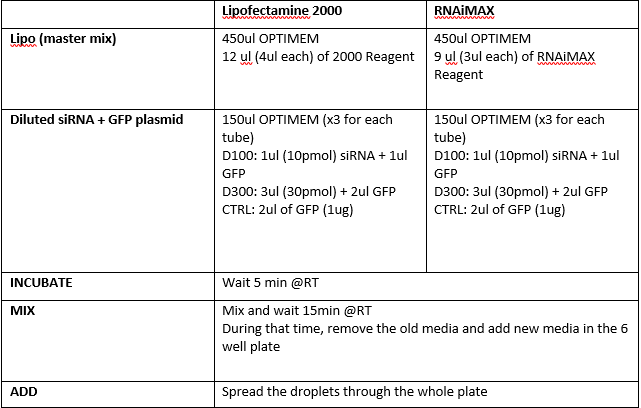
\includegraphics[scale=0.5]{figures/lipo.png}
%	\caption{except I put 15ul instead of 12ul for Lipofectamine 2000 (which is supposed to be less toxic), so 5ul each.}
%\end{figure}

\subsection{Cell viability assay}
Cell viability was assessed with alamarBlue(R) (CHECK!) following the manufacter's protocol. Briefly, 10\% of the total medium volume of the fluorescent solution was added to the cells. After incubation at 37C, 5\%CO2 for 1-4 hours (depending on average cell number), 200 ul of media were extracted and split in a regular and a black 96-well plate (CHECK!). The first plate was used to determine the absorbance of the samples at $\lambda_1$ = 570 nm and $\lambda_2$ = 600 nm. The second plate allowed verification of the first data by obtaining the fluorescence of the samples at $\lambda$ = 585 (CHECK). Both measurements were obtained with POLARstar Omega plate reader (BMG LABTECH).


%The main reagent is Resazurin, a blue and weakly fluorescent dye which emits bright red fluorescence upon its irreversible oxidation. This colorimetric assay is non-toxic which allows repetition of the assay on a three-day period. It is compatible with absorbance and fluorescence reading, which allows us to double-check the results. 

%Life Technologies, US

\subsection{Immunofluorescence}
Coverslips (Cat. no. 631-0149, VWR) were coated with 20ug/ml of laminin (L2020, Sigma-Aldrich) for ReNcell VM cells. The cells are washed twice with PBS and fixed with 4\% PFA (Sigma-Aldrich) for 15 minutes at RT shieded from light. The coverslips are washed 3 x 5 minutes with PBS and permeabilised with 0.2\% Triton X-100 (Thermo Fisher Scientific) in PBS for 10 minutes and washed 3 x 5 minutes in PBS. They are blocked in 3\% BSA (Invitrogen) for 1 hour at RT before primary antibody incubation o/n at 4C (dilutions in table \ref{ABIF}). The cells are washed 3 x 5 minutes in PBS and incubated in the secondary antibodies away from light for 1 hour at RT. The coverslips were washed 3 final times with PBS and were mounted with DAPI (ABCAM MAIS CHECK MIEUX) and sealed with nail varnish.
Image acquisition was done with a Zeiss LSM710 microscope and processed with ZEN software.

%1. Wash 2x with PBS and fix in 4\% PFA for 15 min @RT, away from light
%
%2. Wash the coverslips 2x5min with PBS
%
%3. permeabilise with 0.2\% Triton-X in PBS for 10min at RT.
%
%4. wash with 3x5 PBS and block with 3\% BSA in PBS (=blocking solution) for 1hr.
%
%5 - incubate in primary Ab overnight in blocking solution.
%
%6 - wash 3x5min with PBS 
%
%7 - add secondary Ab in block solution (1:1000) and incubate for 1hr @RT
%
%8 - wash 3x5min with PBS (away from light)
%
%9 - mount on slide with DAPI and seal with nail varnish.

%Remove the medium of cells, fix with 4\% PFA for 10 minutes (on shaker), wash 3x5 minutes with PBST (=PBS + 0.1\% Tween). 
%Incubate the cells for 1h with blocking solution (at room temperature on the shaker as well).
%In a back chamber, add paper + distilled water, flatten, parafin and add 50ul of primary Ab.

%Primary AB:
%
%1) (L4) Tuj1 - MOUSE (Biolegend, 801202) - 1:100
%
%2) (G11) Sox2 - RABBIT (CST, 3579P) - 1:400
%
%3) (H2) GFAP - RAT (Invitrogen, 13-0300) - 1:100
%
%Leave overnight and wash 3*5min with PBST. 
%
%Secondary antibodies must simply recognise the animal used in the other antibody. Here:
%
%1) (A1) MOUSE - Alexa 488 A11029 (LifeTechnologies) - 1:1000
%
%2) (C6) RABBIT - Alexa 594 A11037  (LifeTechnologies) - 1:1000
%
%3) (E9) GOAT - Alexa 647 A21247  (LifeTechnologies) - 1:1000
%
%Same as before, put 50ul of Ab on the parafilm, then drop the cover slip cells first on the drop, leave on for 40 min @RT in the black chamber, then rinse 2x5min with PBST and 1x5min with PBS. Put the coverslips on the slides and seal with nail varnish.  


\begin{table}[]
	\centering
	\caption{Antibodies used in IF
	Also I used TUB3 for SY5Y second staining, for the rest, the us'}
	\label{ABIF}
	\begin{tabular}{@{}ccccccc@{}}
				\rowcolor{white}
		\toprule
		\textbf{Protein} & \textbf{Species} & \textbf{Dilution} & \textbf{Cat. no.} & \textbf{Company} & \textbf{Target}                                                              & \textbf{Secondary antibody} \\ \midrule
		SOX2             & Rabbit           & 1:400             & 3579P                 & CST              & \begin{tabular}[c]{@{}c@{}}Marker for\\ stem cells\end{tabular}              & Alexa Fluor 594             \\
		Nestin           & Goat             & 1:100             & sc-21248              & Santa Cruz       & \begin{tabular}[c]{@{}c@{}}Marker for\\ stem cells\end{tabular}              & Alexa Fluor 488             \\
		MAP2             & Rabbit           & 1:200             & 8707                  & CST              & \begin{tabular}[c]{@{}c@{}}Marker for mature\\ neurons\end{tabular}          & Alexa Fluor 594             \\
		Tuj1             & Mouse            & 1:100             & 801202                & Biolegend        & \begin{tabular}[c]{@{}c@{}}Marker for mature\\ neurons (fibers)\end{tabular} & Alexa Fluor 488             \\
		Olig1            & Mouse            & 1:100             & MAB1327               & RD Systems       & \begin{tabular}[c]{@{}c@{}}Marker for mature\\ oligodendrocytes\end{tabular} & Alexa Fluor 647             \\
		GFAP             & Rat              & 1:100             & 13-0300               & Invitrogen       & \begin{tabular}[c]{@{}c@{}}Marker for glial\\ cells\end{tabular}             & Alexa Fluor 647            
	\end{tabular}
\end{table}

\subsection{Western blot}
Cells were put on ice and rinsed with ice-cold PBS twice. After removing any trace of PBS, lysis buffer (composition of LB in Table \ref{LB} and \ref{RIPA}) was added and  the plates were scraped, transferred in chill 1.5ml tubes. We vortexed the samples thoroughly, let them sit 30 minutes on ice and sonicated 5 for 5 pulses at power = 20. 
Cells were centrifuged at 14 000 rpm for 10 minutes at 4C. Transfer the supernatant in clean chilled tubes and determine protein concentration with a BCA assay. 


\subsubsection{BCA assay}
Protein concentration was established following the Pierce BCA Protein Assay Kit (Thermo Scientific) with Pierce bovine serum albumin standards. In a 96-well plate, samples and standards were duplicated. After adding the Working Reagent (Thermo Scientific), the plate incubated at 37C for 30 minutes before measuring the absorbance ($\lambda$ = 620 nm) with a POLARstar Omega plate reader (BMG LABTECH).

%
%
%Preparing samples: http://www.abcam.com/protocols/sample-preparation-for-western-blot
%ATTENTION: when you lysate the cells, you want to make sure that you remove ALL the PBS, let the cells dry a little before adding the lysates (in order to get high concentrations of protein since you can only load a restricted volume!).
%
%As written (but RIPA used as base and you add cockaail of inhibitors, blabla), then you let rest for 30min while vortexing every 10 min (for 30s/sample) and finish with 5 pulses of sonication (at power 20 and pulses = 50 - 5 pulses) to get rid of any residue (be sure that the lysate is homogenous). then, centrifuge at 4C at 14000rpm for 10 min. Transfer the supernatant in clean chilled tubes. 
%g
%Protein concentration was determined with a BCA assay (standards with Albumin at 2mg/ml, done following the kit ThermoIns)

%The samples were completed with RIPA or loading buffer to get equal protein load (between 20 and 40 ug). 
%The loading buffer used was a NuPage$^{\text{TM}}$ LOADING BUFFER (??) combined to DTT [stuck at 20X, must reduce to 4X] (a reducing agent which reduces disulfide bonds: such residual structure could lead to disrupted migration). 



%
%Must get the sample buffer = lysis buffer (blue) + DTT (stock 20X) which must all be at 4X. 
%Complete the lysates according to the Excel sheet (must find the smallest volume and use that for the rest).

%cook at 95C for 10 minutes, centrifuge 1min at 7 400 to pull the evaporation, then store at -20C. 

%When running the blot, cook at 95C again, centrifuge and keep on ice. Then, 

\subsubsection{Bradford assay}
%One must be sure that the Omega reader is available (so book it before doing the Bradford since the shorter the wait before the analysis, the better).
%The Bradford assay is in the fridge on Frances/Dafni/Marias' side, in the bottom well - ask Luana if you can't find it - and my standards are in the green box in our fridge.
Protein concentration for limited volume samples was established using Coommassie Blue (). In a 96-well plate, samples and standards were pipetted in triplicates of 1ul and 200ul of Coommassie Blue were added. After mixing thoroughly and removing any bubble, the absorbance at $\lambda$ = 595nm was measured with a POLARstar Omega plate reader.


\subsubsection{Running the gel}
The samples were denatured at 90C for 10 minutes and centrifuged briefly before loading on pre-cast NuPAGE$^{\text{TM}}$ 4-12\% Bis-Tris Protein gels. They were run at 120V for approximately one hour in SDS MOPS running buffer (NuPage) and transferred on a methanol-activated nitrocellulose membrane at 100V for one hour in ice-cold transfer buffer. The membrane was then washed and blocked for an hour at room temperature in blocking buffer (PBS + 0.1\% Tween + 5\% milk) before incubating overnight at 4C in the primary antibodies. 
(?) Checker Tween
The membrane was then washed three times in PBS-T and incubated 1 hour at room temperature in secondary antibodies. Finally, the membrane was washed again and covered in ECL for one minute to then be developped. 


%Using a NuPAGE$^{\text{TM}}$ 4-12\% Bis-Tris Protein Gels and SDS MOPS running buffer (stock at 20X, dilute in distilled water, 950ml of H20, 50ml of stock), add the gels (facing the interior), fill to the rim (more or less), order the samples, then determine how much to load to get same concentrations. 
%Add 5ul of ladder (ideally between each set of samples), and then load.
%Set to 120V for about 1 hour (check regularly ). WHILE THIS IS RUNNING, add 1L of transfer buffer to the cold room.
%
%Transfer to membrane:
%Using the transfer buffer, with a 2 sponges, 2 black things, two blot papers and one membrane (nitrocellulose) per gel, drop it in methanol (at least 10sec) and start the sandwich (with everything wet in transfer buffer): with the black facing the bottom, add the black+sponge+blot+gel+membrane+blot+sponge+black and close. In the transfer box, add a magnet + a block of ice and set with the black touching the black. Run for 1hr at 100V. 


%FIRST STAIN:
%Add ponceau red, then wash with PBST and check for band.
%Wash with PBST then block in milk (5\%) for an hour.
%
%
%TRANSFER BUFFER = H20 (7l) + (1l) Transfer Buffer (20X) + (2l) Methanol. 
%
%
%- block for one hour
%- transfer to the falcon tubes with the primary Ab (3ml/tube) and leave at 4C overnight.
%- wash 3x5min with PSBT and prepare 2ndary AB in 5ml each (if twice same animal, can put the membranes together, here it's the case for rabbit):
%1) rabbit: 1:5000
%2) mouse: 1:5000.
%- shake @RT for 45min. 
%
%- wash 3x5min with PBST.
%
%- ECL + develop. 
%
%
%Cut in three pieces: over 100 (Lats2), 55-100 (YAP + DYRK1A) and 20-55 (Casp9):
%First round of primary antibodies:
%- pLats2, DYRK1A, Casp9
%
%1) pLATS2 (rabbit): F2 Novus 4C      1:1000 (3ul)
%2) DYRK1A (rabbit): D7 Santa Cruz 4C    1:500 (6ul)
%3) Caspase 9 (mouse): D9 9508 CST -20C    1:1000 (3ul)
%
%
%16.05.18:
%1) Ki67 (300kda rabbit): F18 AB9260 Millipore 4C      1:1000 (3ul)
%2) pYap (rabbit): J21 Santa Cruz -20C    1:1000 (6ul)
%3) Caspase 9 (mouse): D9 9508 CST -20C    1:1000 (3ul)
%For this, you use the stripping buffer which is 13ml of NaOH (10M) and 7ml of SDS 10\%, complete with 250ml of distilled water.
%
%So, you wash with distilled water once over quickly, then add the stripping buffer for X minutes (shaker @RT), then wash 3x5min with PBST. Then you can transfer in the primary Ab straight away. REMINDER - in primary Ab, always add NaN3 (1:500) to preserve (Sodium Azide( )!
%(different lengths of stripping depending on the strength of signal on the first blot - 10min MAX).
%Then wash 3x5min in PBST
%
%Ideally, next round:
%
%1) pYAP, different Ab?]
%2)
%
%
%
%
%Second round:
%- pYAP, (Lats2?),  + Casp again, Loading control
%
%1) 
%2) K17 pYAP (mouse): sc-101199 SC 4C 1:1000 (3ul)
%3) Caspase 9 (mouse): D9 9508 CST     1:1000 (3ul)
%
%23.5.18: 
%Loading control: Alpha Tubulin 1:2000 (H16 at -20, Rabbit, 2125s CST).
%p-TYR on DYRK1A (L13 at 4deg, Mouse, sc-7020). 


\begin{table}[]
	\centering
	\caption{Primary antibodies used in WB. They were diluted in blocking buffer with 1:500 sodium ozide.}
	\label{AbWB}
	\begin{tabular}{ccccc}
		\rowcolor{white}
		\hline
		\textbf{Protein}  & \textbf{Species} & \textbf{Dilution} & \textbf{Cat. no.} & \textbf{Company} \\ \hline
		Caspase 9         & Mouse            & 1:1000            & 9508S                 & CST              \\
		Cleaved Caspase 3 & Rabbit           & 1:1000            & 9661S                 & CST              \\
		DYRK1A            & Rabbit           & 1:1000            & sc-130741             & Santa Cruz       \\
		GAPDH             & Rabbit           & 1:1000            & AB128915              & Abcam            \\
		p-Thr-Pro         & Mouse            & 1:1000            & 9391S                 & CST              \\
		RASSF1A			  & Mouse			 & 1:1000			 & AB23950				 & Abcam			\\ 
		SIRT1             & Mouse            & 1:1000            & 8469S                 & CST              \\
		YAP               & Rabbit           & 1:1000            & 4912S                 & CST           
	\end{tabular}
\end{table}


\begin{table}[!htb]
	\begin{minipage}{0.5\linewidth}
		\centering
		\caption{Composition of lysis buffer used for the western blots (scaled for 1.5ml)}
		\label{LB}
	\begin{tabular}{lll}
				\rowcolor{white}
	\bottomrule
	\textbf{Component} & \textbf{Stock} & \textbf{Volume} \\
\bottomrule
	Na$_3$vO$_4$      & 1x &    1.5 uL                 \\
	$\beta$-glycerophosphate     & 1X  &    15 uL              \\
	Protease inhibitors      & 50X &    30 uL              \\
	NaF      & 1X &    150 uL              \\
	RIPA buffer   & 1X &    1 303.5 uL   \\      
\end{tabular}
	\end{minipage}%
\hspace{2em}
	\begin{minipage}{.4\linewidth}
		\centering
		\label{RIPA}
		\caption{Composition of radioimmunoprecipitation assay (RIPA) buffer.}
	\begin{tabular}{ll}
				\rowcolor{white}
\bottomrule
	\textbf{Component} & \textbf{Stock}  \\
\bottomrule
	Sodium deoxycholate     & 0.5\%                 \\
	EDTA     & 5mM               \\
	Tris-HC      & 50mM               \\
	NaCl      & 1X        \\
	NP-40   & 1\%         \\
\end{tabular}
	\end{minipage} 
\end{table}

%\begin{table}[h]
%	\centering
%	\caption{Composition of lysis buffer used for the western blots (scaled for 1.5ml).}
%	\label{LB}
%	\begin{tabular}{lll}
%		Component & stock & volume (uL) \\
%		Na$_3$vO$_4$      & 1x &    1.5                 \\
%		$\beta$-glycerophosphate     & 1X  &    15               \\
%		Cocktail of protease inhibitors      & 50X &    30               \\
%		NaF      & 1X &    150               \\
%		RIPA buffer   & 1X &    1 303.5            
%	\end{tabular}
%\end{table}         
%
%\begin{table}[h]
%	\centering
%	\caption{Composition of radioimmunoprecipitation assay (RIPA) buffer.}
%	\label{LB}
%	\begin{tabular}{ll}
%		Component & stock  \\
%		Sodium deoxycholate     & 0.5\%                 \\
%		EDTA     & 5mM               \\
%		Tris-HC      & 50mM               \\
%		NaCl      & 1X        \\
%		NP-40   & 1\%           
%	\end{tabular}
%\end{table}        

\subsection{Bioreactor simulation}
Using Autodesk Inventor Professional 2019 and Autodesk CFD 2018 with a student licence - maybe COMSOL Multiphysics??

The prototypes were built on Autodesk Inventor Professional 2019 using the same technique catered to various designs: drawing the 2D base, extruding it to obtain a 3D model then exporting this raw file to the CFD 2018 Module. One must then set the material (here, we approximated the medium to plain water) and the boundary conditions. For the inlet, we set the volume flow to 10uL/hr. This value stems from static culture comparison: 

 \begin{equation}
 \text{inlet flow} = \frac{\text{volume per well}}{\text{frequency of medium change}} = \frac{500\text{ uL}}{48 \text{ hours}}
 \end{equation}
 
 The oulet condition is pressure since the our set up does not use a pump on the outlet side. To visualise the mixing capacity of a prototype, the initial volume is filled with water and the scalar "0" (colour red), and the inlet lets scalar "1" in, mimicking the influx of new medium. This is a way to show two liquids mixing, with assumed mass diffusivity constant of 2.10$exp{-5}$. This is the diffusion coefficient of oxygen in water. 
 Note: our bioreactor simulation has a capacity of about 785ul (and we add about 10ul/hr).

\subsection{Casting bioreactor}
The bioreactor is made of polydimethylsiloxane, or PDMS, which is a form of silicone. It is achieved by mixing the polymers (Sylgrad 184 Silicone Elastomer, Dow Corning) and the cross-linking reagent (Sylgard 184 Silicone Elastomer Curing Agent, Dow Corning) with a 10:1 ratio, which is then poured in the mould. It is then put into a vacuum chamber for one hour to allow encased bubbles to surface up and be removed. Finally, the bioreactor must bake in a 60°C oven for 24 hours. It is then removed from the mould and autoclaved before use. 

\subsection{Radiation}
Either with concentrating beam
Or with the shielding thing. DIFFERENT. 
- changed the medium of all cells before radiation every time. (IF ADDING DRUGS, should add right before the radiation rather than after, that means no need to change the milieu after)

- briefly explain how x-ray generators work, to factor in the heel effect (check dans les favoris, le site est super clair nde-ed). 
- explain why we chose x-rays and not alpha-particles for instance: x-rays are the most relevant form of radiation in the in vitro context since the purpose would be to transfer such findings in the clinic, where x-rays are still the standard treatment.
- use of 225kv and 17mA on the EXP 1 (96 well plate, for 1.25min - more or less 2Gy).
- use of 250kV and 12mA on the EXP 2 (24 well plate, exactly 2Gy).

"PROTOCOL":
- new 'machine' to automate the movement of the plate depending on how it must be radiated (so that one needn't enter the room every time to change the placement of the lead - ultimately renders the experiments a lot more reproducible). Still in development so we chose to sacrifice the 8th column in half. 


\subsubsection{Dosimetry}
Initial step was to put the motors and set them to the plate+field size. Then add a film (just to get a feel of the dose distribution) --> got a good distribution (cannot see a heel effect just by looking at the film transcript).

Heel effect: The end result is that the field intensity towards the cathode is more than that towards the anode (due to electrons traversing the target and having to escape it - many are resorbed). Described in my book. 
This is compensated (partially) by a 'heel effect compensation' filter (which also hardens the beam to get rid of 'useless' soft x-rays) which is made of concentric copper rings. 
 

Use of collimator to get a fairly high dose-rate while limiting scatter and achieving a homogeneous dose distribution.

\subsubsection{Protocol?}  




\subsection{Oxdidative stress assay}
The extent of oxidative stress was determined with a dichloro-dihydro-fluorescein diacetate (DCFH-DA) assay. The DCFH-DA (Sigma-Aldrich) was diluted in DMSO to a stock concentration of 10mg/ml (1000X).

\subsubsection{Microscopy}
The cells were rinsed gently twice with PBS, before adding DCFH-DA further diluted to 1X in PBS. They were incubated at 37C, 5\%CO2 shielded from light for 30 minutes. Image acquisition was performed with a (CHECK WHICH MICROSCOPE, LITTLE OR RHOD?). 

\subsubsection{Flow Cytometry}
The cells were washed gently twice with PBS and detached with Trypsin (SY5Y cell line) or Accutase (ReNcell VM). They were then spinned down at 300g x 5 minutes at 4C and washed twice with FACS buffer (2\% FBS + 2mM EDTA in PBS) in round-bottom 96-well plates. They were resuspended in DCFH-DA further diluted to 1X in PBS and incubated at 37C, 5\%CO2 for 30 minutes before being exposed to 2 Gy of x-rays in suspension. They were kept on ice and analysed straight-away with an Attune Autosampler NxT Flow Cytometer (Thermo Fisher). 

\subsection{Statistical analysis}
Statistical analysis was performed with GraphPad Prism 7 (version 7.1, GraphPad Software, Inc.). Shapiro-Wilk normality test was performed on every data set to assess the distribution. The standard variation of comparable sets was checked to justify the use of Welch's correction on the unpaired T-test. A parametric or non-parametric (Mann-Whitney for non-Gaussian distributions) t-test was then performed to investigate any significant difference.  


\section{Results}
\subsection{Characterisation of the SY5Y and ReNcell VM cell lines}
\subsubsection{The ReNcell VM cell line}
According to the workflow depicted in Figure \ref*{workflow},  the cells were plated on Day 0 in complete medium which was changed to differentiation medium on Day 1 (with or without drug inhibitors). This was maintained for 4 days to allow significant differentiation. Finally, the cells were radiated with 2 Gy x-rays and kept to grow for 2 more days before being harvested.  

In this context, their differentiation pattern was assessed with immunofluorescence over 21 days of culture in maintenance medium. 
 The results of the 5 time points can be found in Figure \ref{diff-vm}. This characterisation assay revealed an important feature of ReN VM cells which is their ability to express a wide array of markers. The Figure \ref*{stain-opti}.A sums up the markers used in neural stem cell culture to determine differentiation. Instead of the binary dogma of positive or negative cells, the VM cells were positive for each marker. This was further verified by comparing different antibody stains on Day 14 and Day 21 (not shown) differentiated cells on \ref*{stain-opti}.B. The antibodies were chosen according to the Abcam's neural marker guide and availability in the laboratory's stock. Once again, the cells were positive for both stem cell markers (Nestin and SOX2) and an array of differentiated neural cells (immature neurons with $\beta$-III tubulin, now referred to as Tuj1, oligodendrocytes with Oligo1 and radial glia with GFAP).

%The strength of the SOX2 signal was the one that varied the most between the 5 stages of differentiation but 

It was thus tricky to rely exclusively on the immunofluorescence signal of each marker. Instead, the differentiation stage was determined using the morphology. Indeed, the cells increasingly elongate as they differentiate and form neurites, which is reflected in both Tuj1 and GFAP stains. The whole cell body size decreases as well as they thin out and extend to form connexions with nearby cells.

%Finally, the sharpness of the signal is a good marker of differentiation: indeed, on Day 0 and 3, a proportion of cells have a diluted Tuj1 signal (red boxes) which becomes sharper. 

\newpage
\begin{figure}[h]
	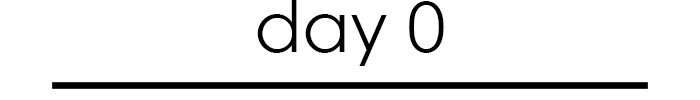
\includegraphics[width=0.196\textwidth]{figures/IF/charac(light)/d0}
	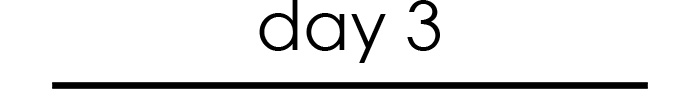
\includegraphics[width=0.196\textwidth]{figures/IF/charac(light)/d3}
	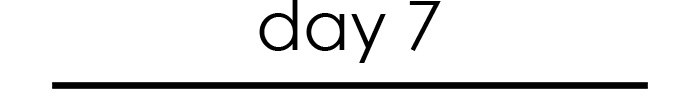
\includegraphics[width=0.196\textwidth]{figures/IF/charac(light)/d7}
	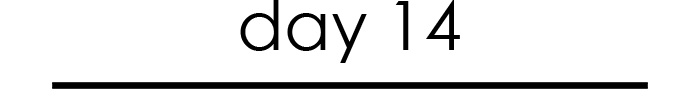
\includegraphics[width=0.196\textwidth]{figures/IF/charac(light)/d14}
	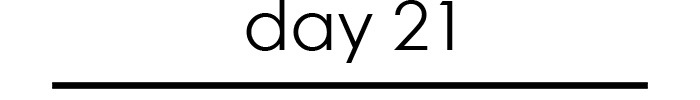
\includegraphics[width=0.196\textwidth]{figures/IF/charac(light)/d21}
	
	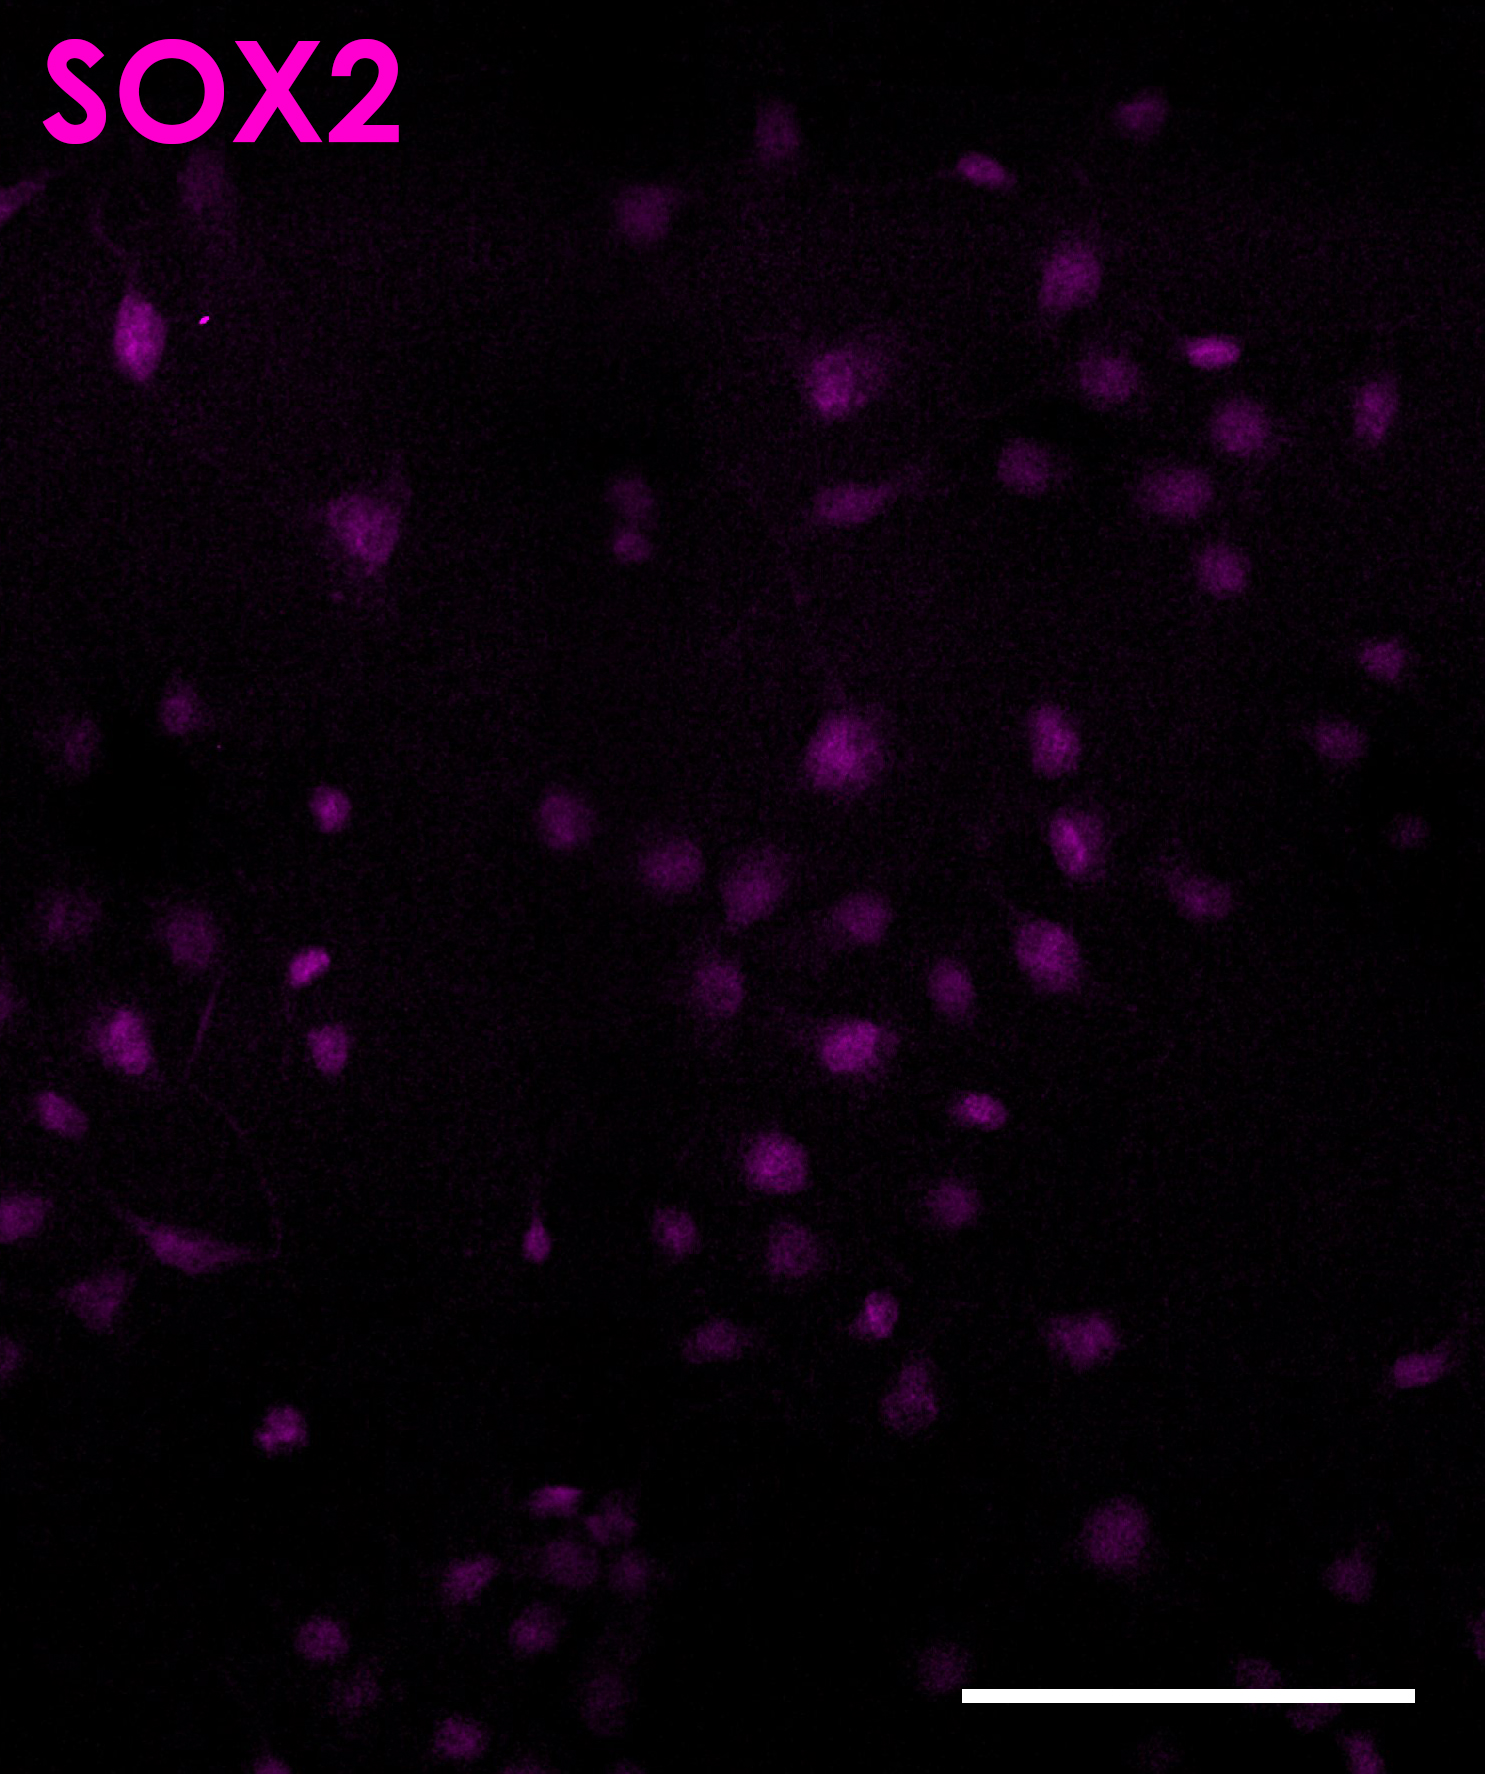
\includegraphics[width=0.196\textwidth]{figures/IF/charac(light)/d0-s}
	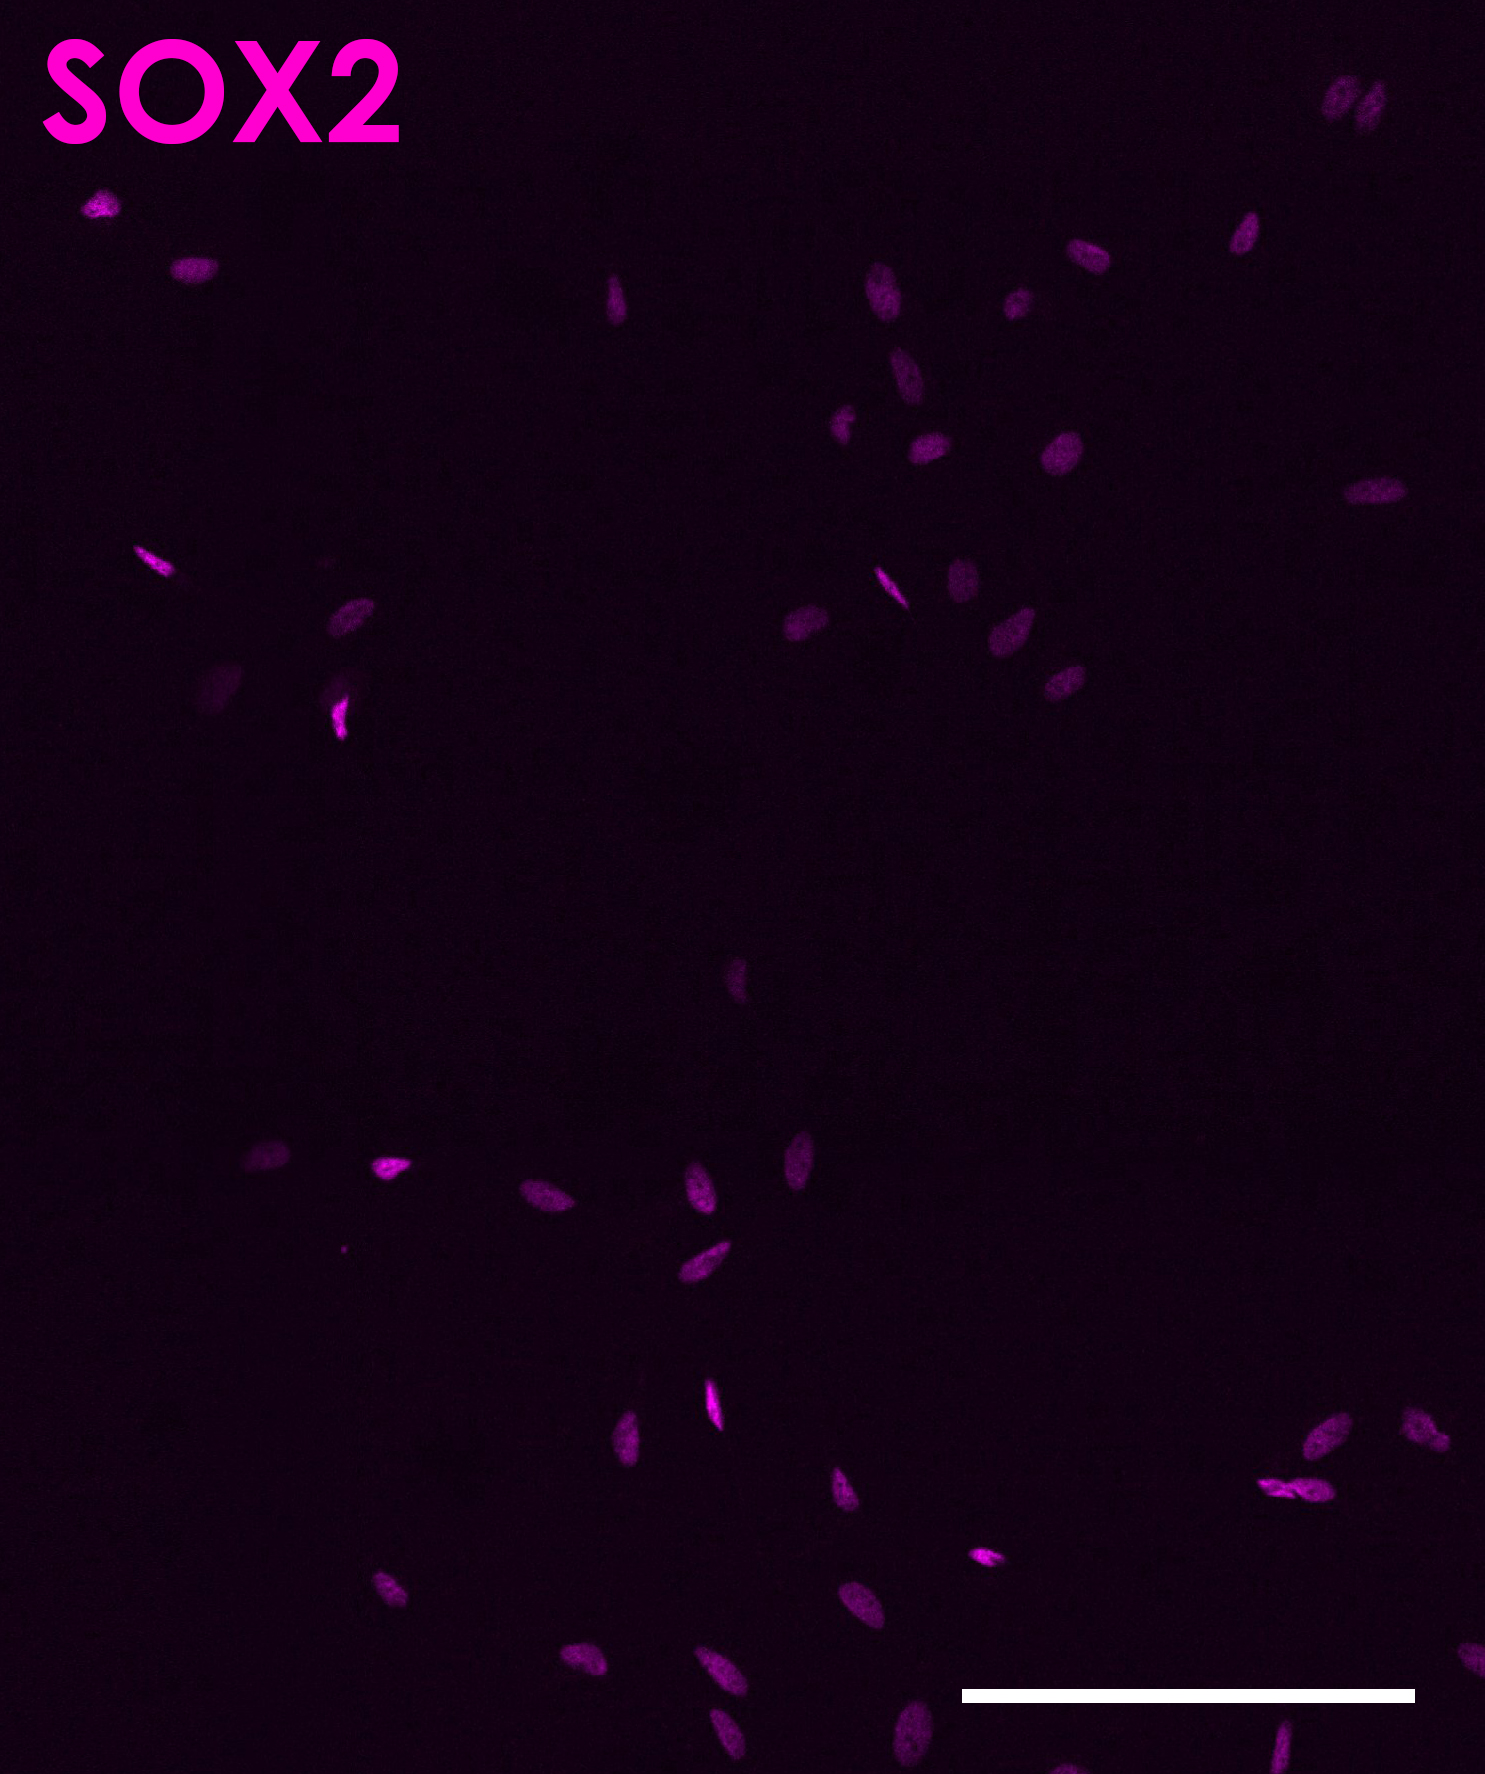
\includegraphics[width=0.196\textwidth]{figures/IF/charac(light)/d3-s}
	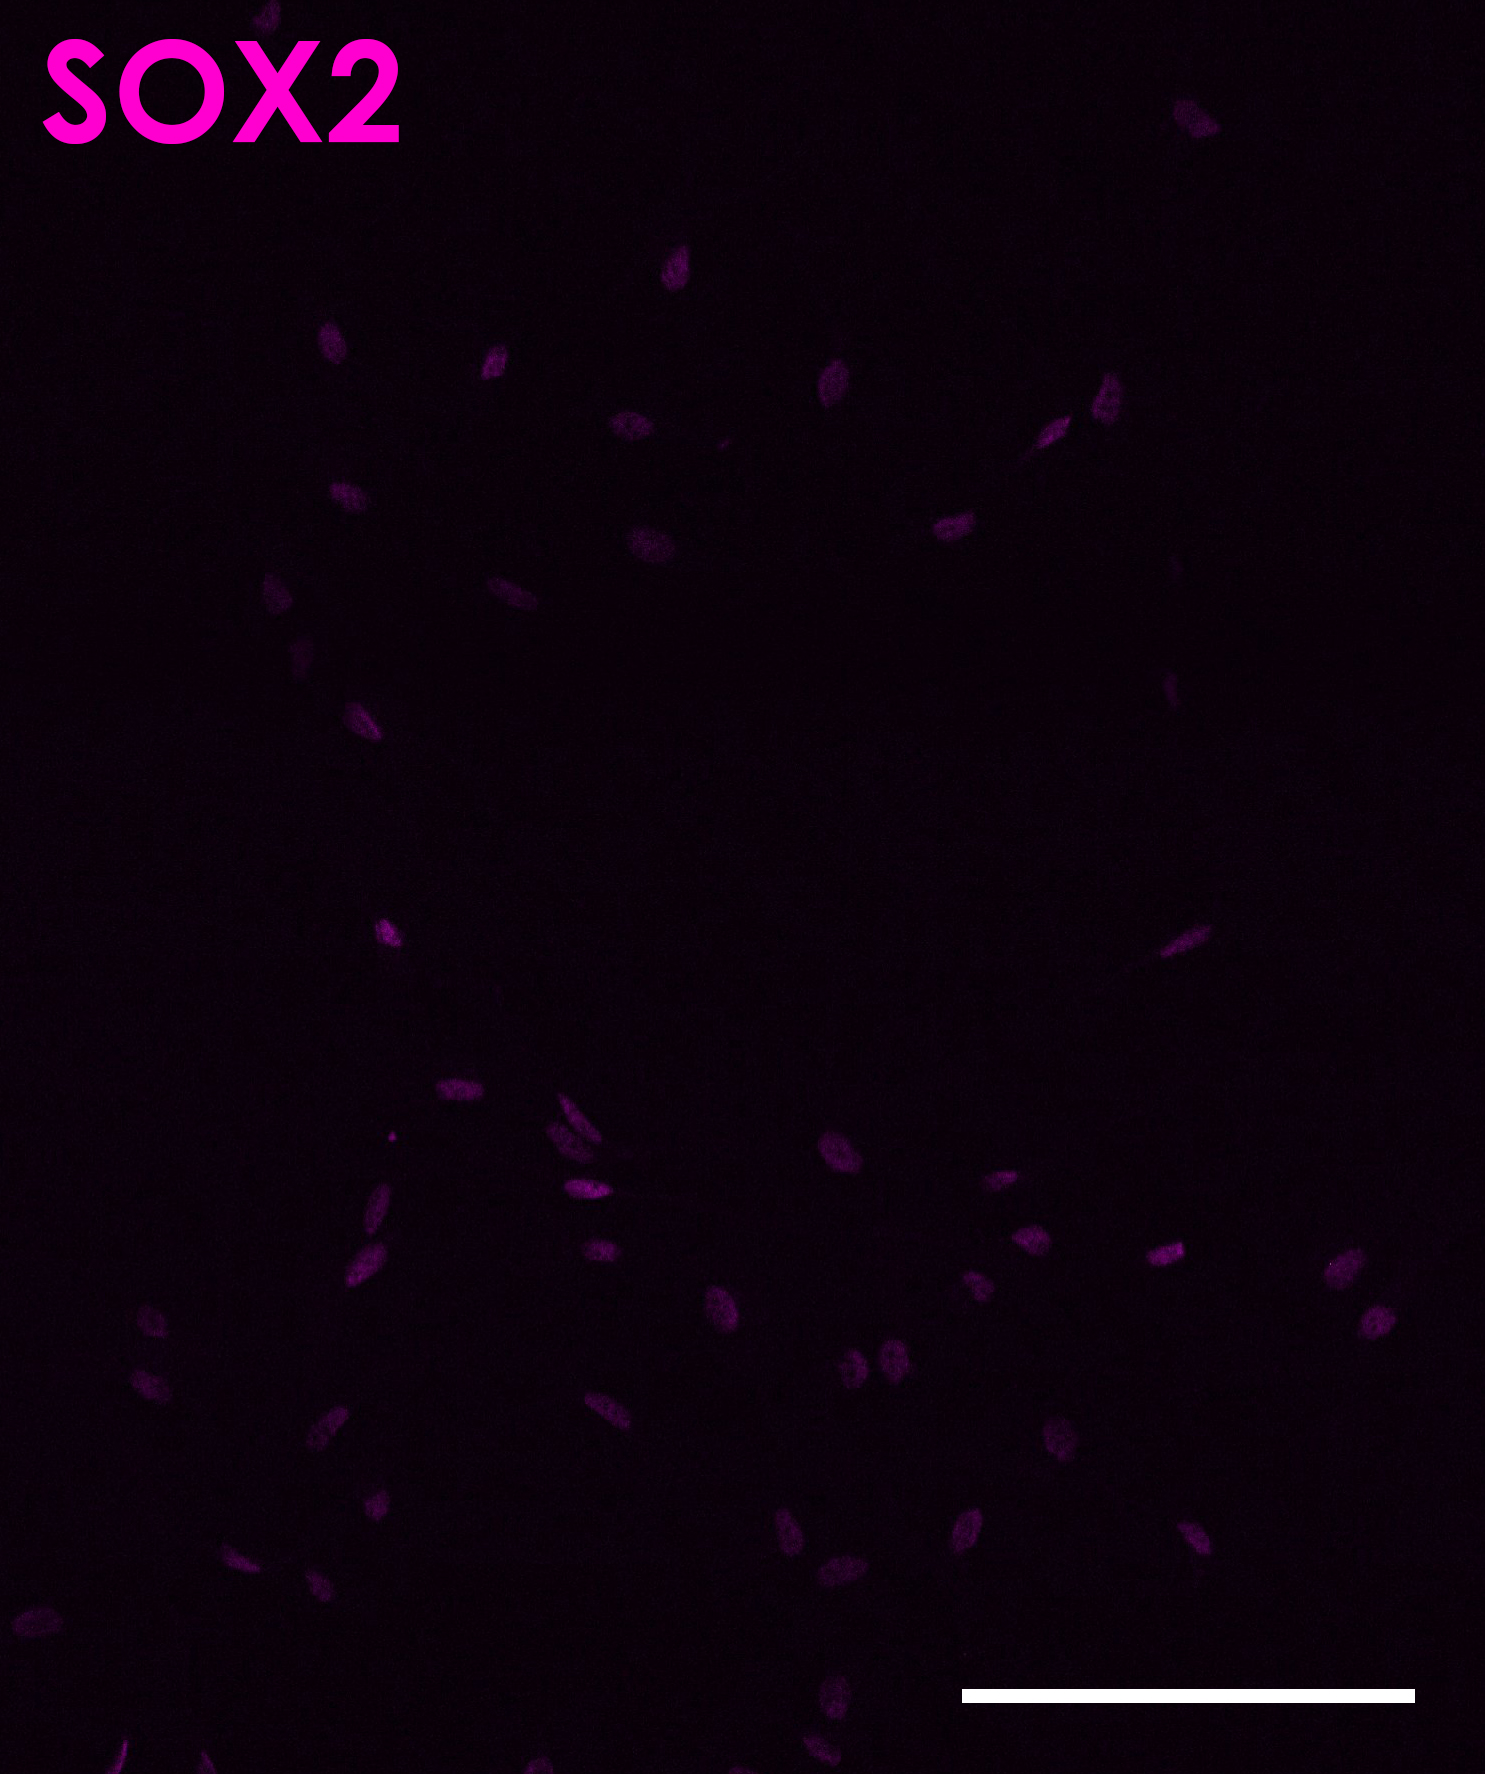
\includegraphics[width=0.196\textwidth]{figures/IF/charac(light)/d7-s}
	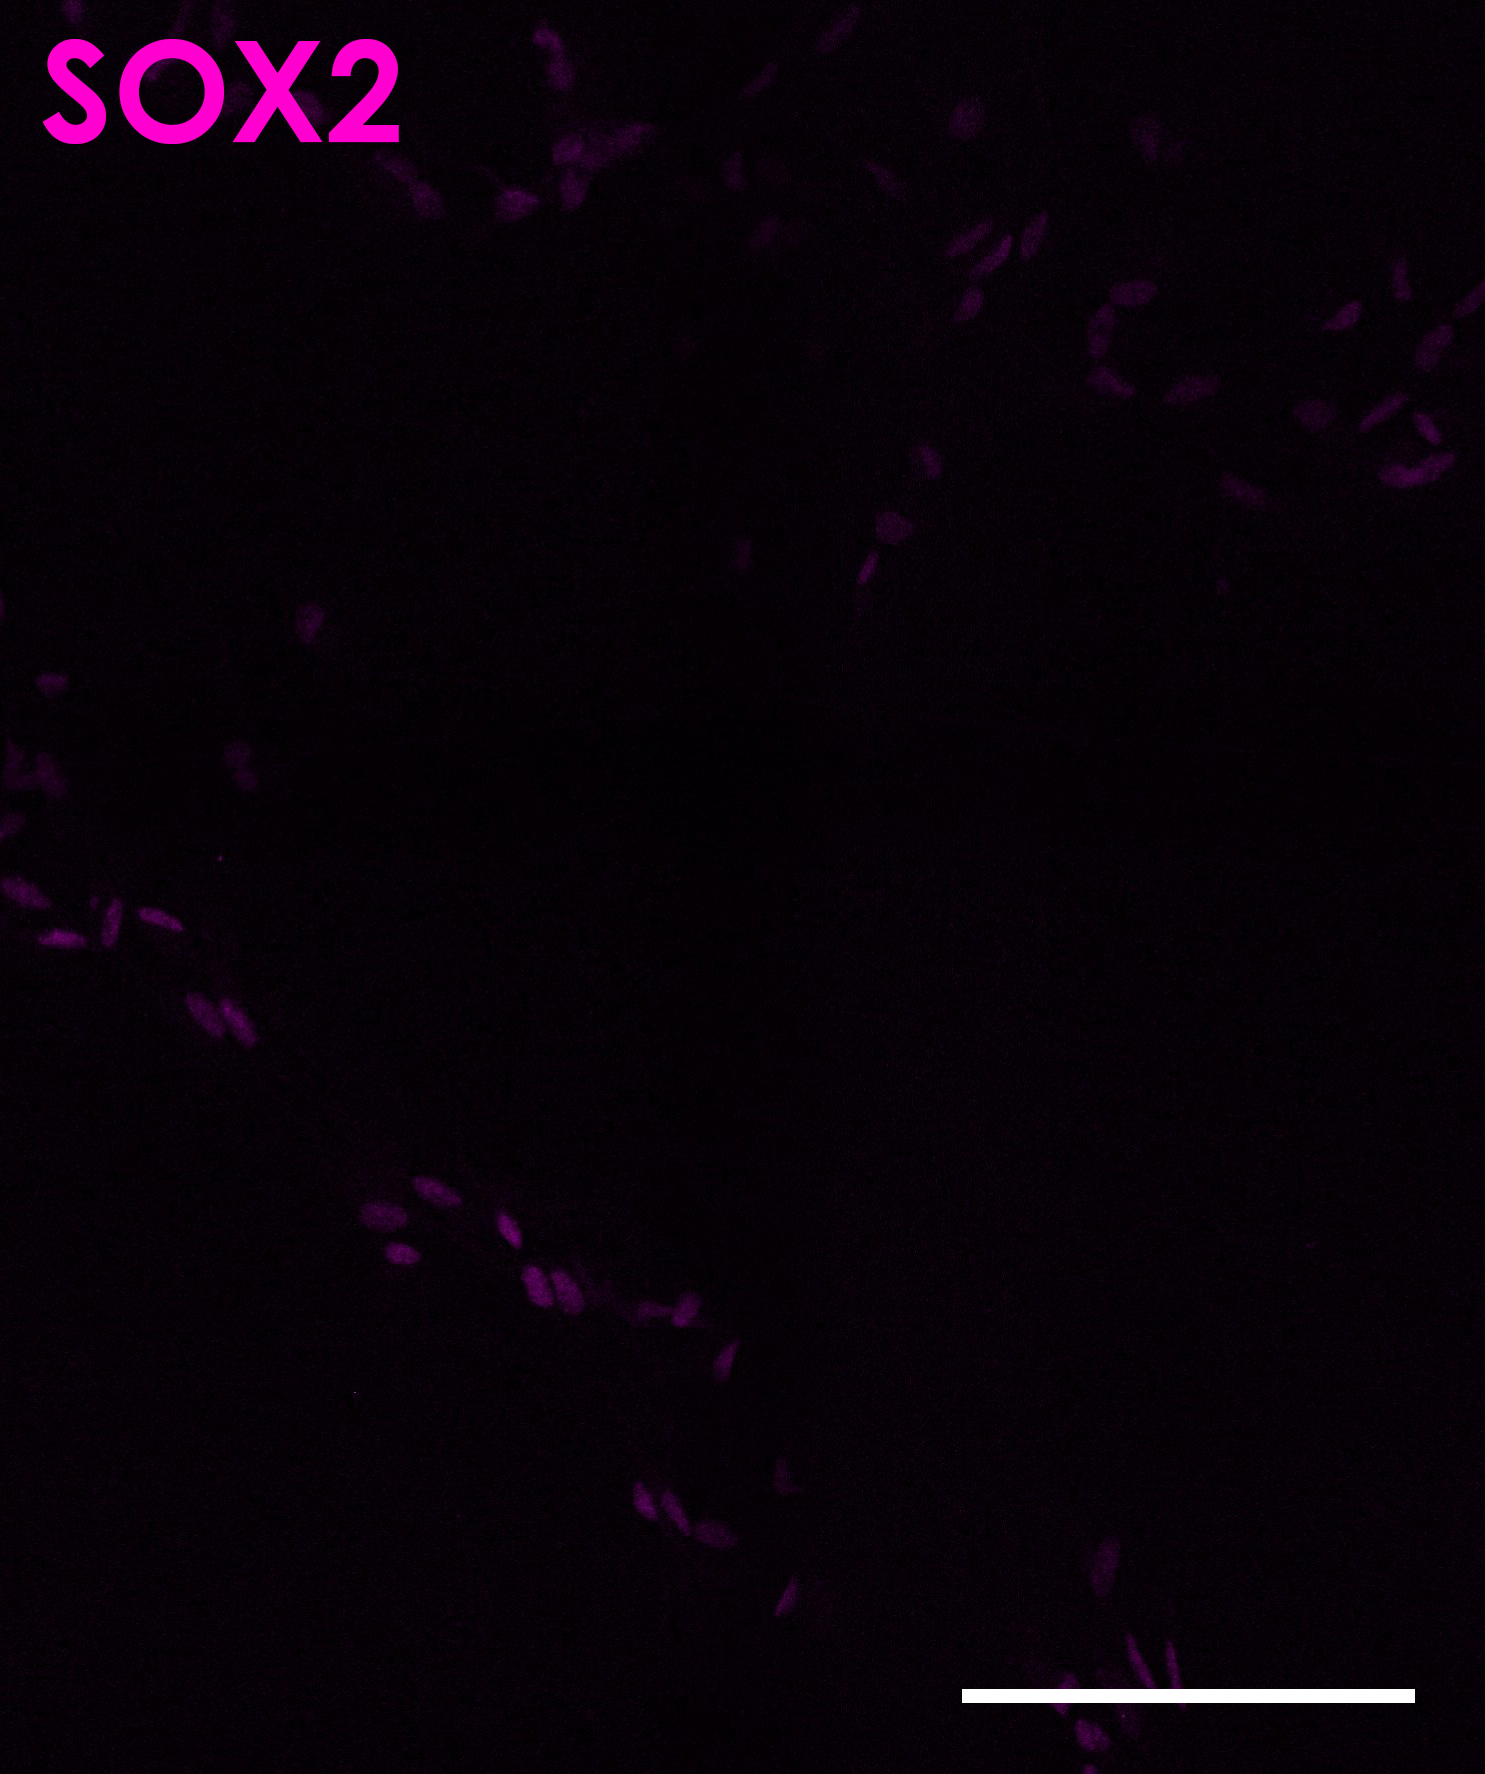
\includegraphics[width=0.196\textwidth]{figures/IF/charac(light)/d14-s}
	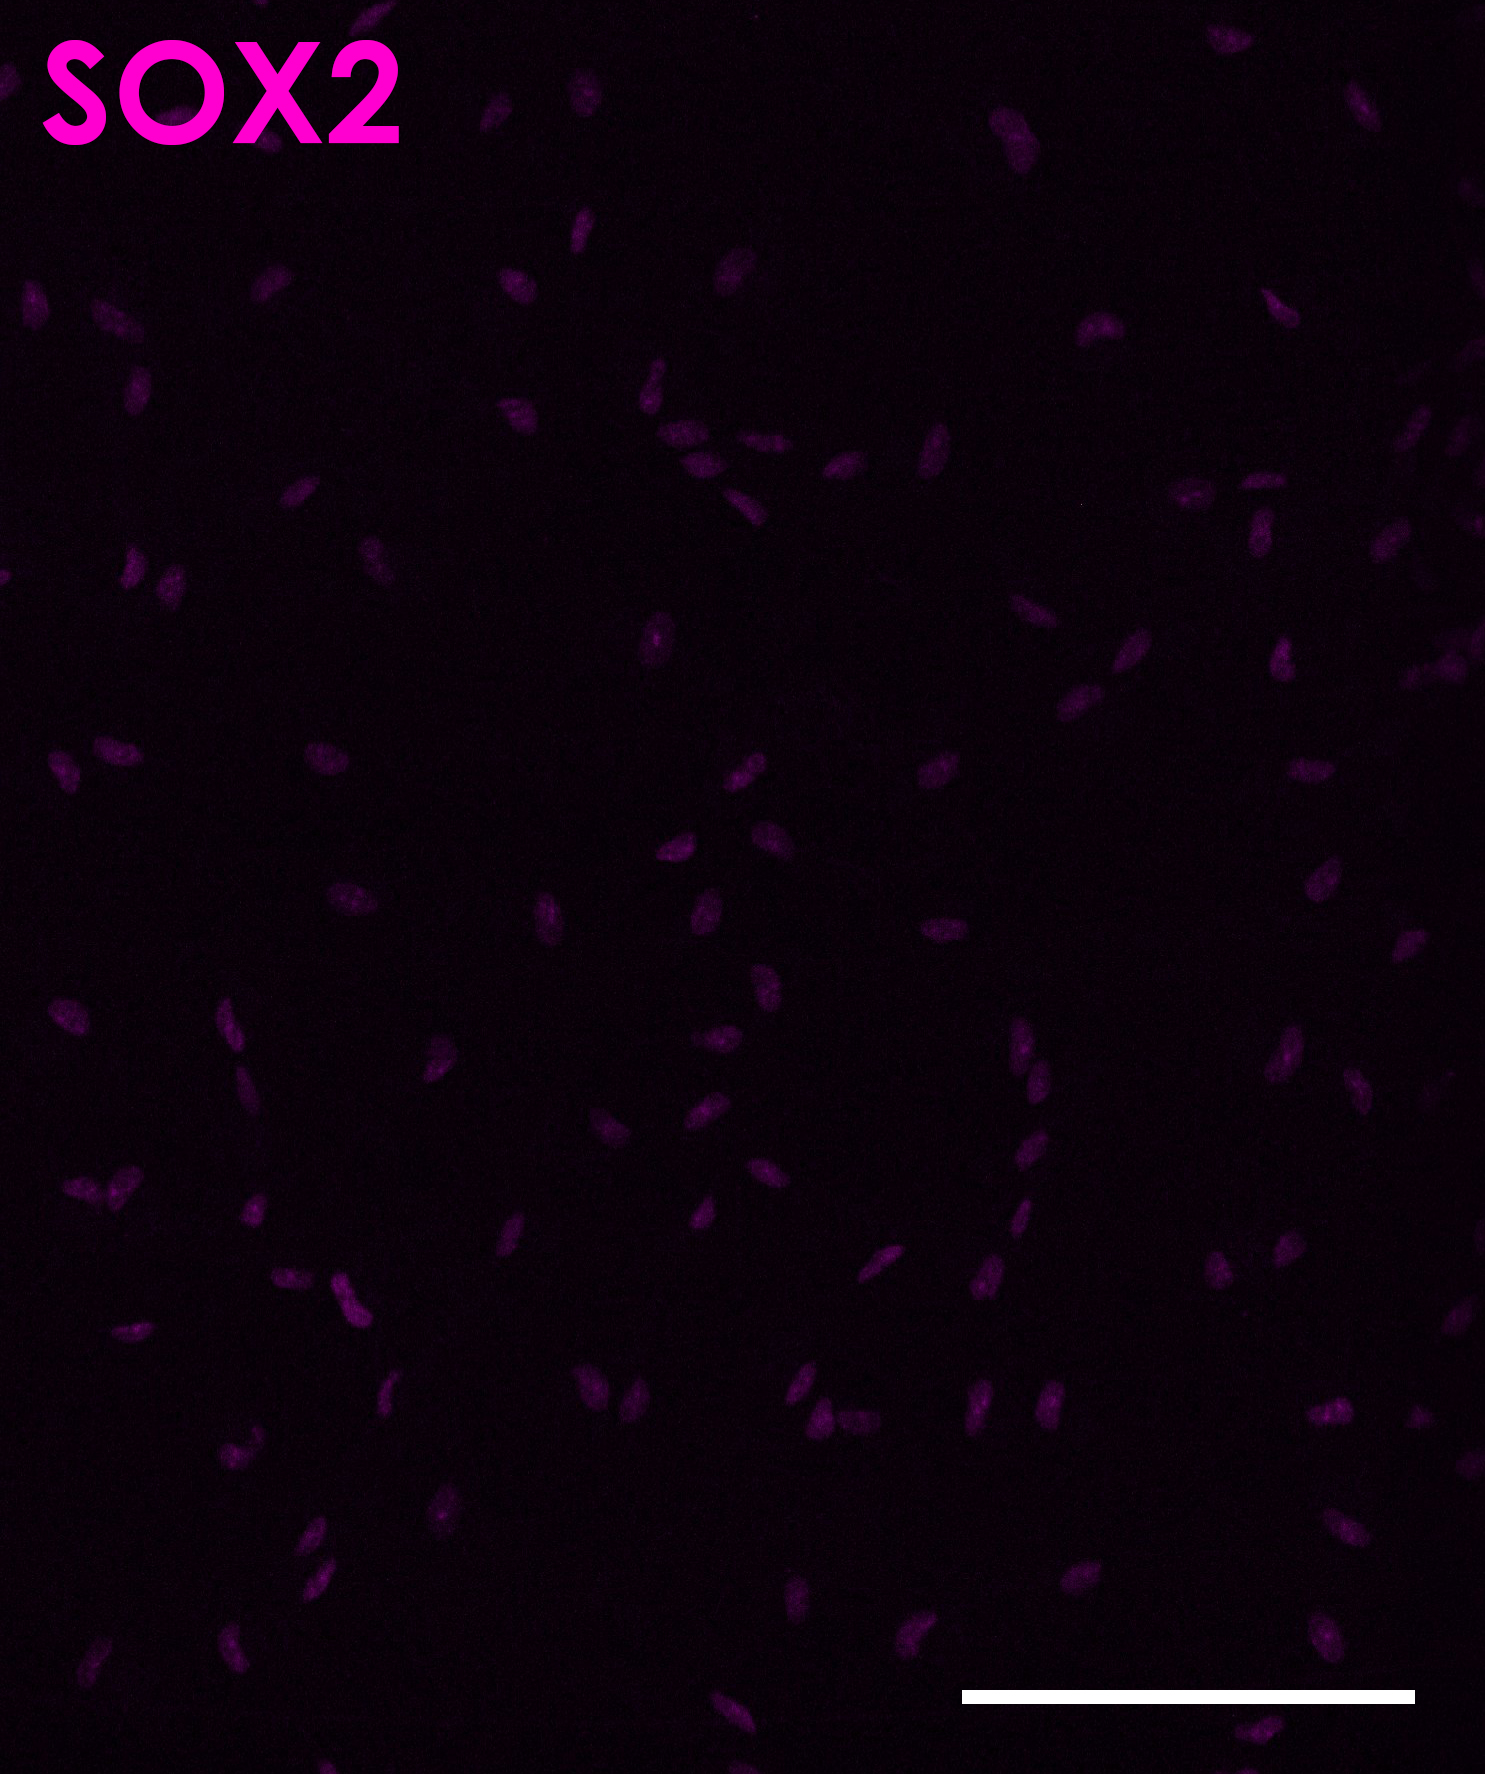
\includegraphics[width=0.196\textwidth]{figures/IF/charac(light)/d21-s}
	
	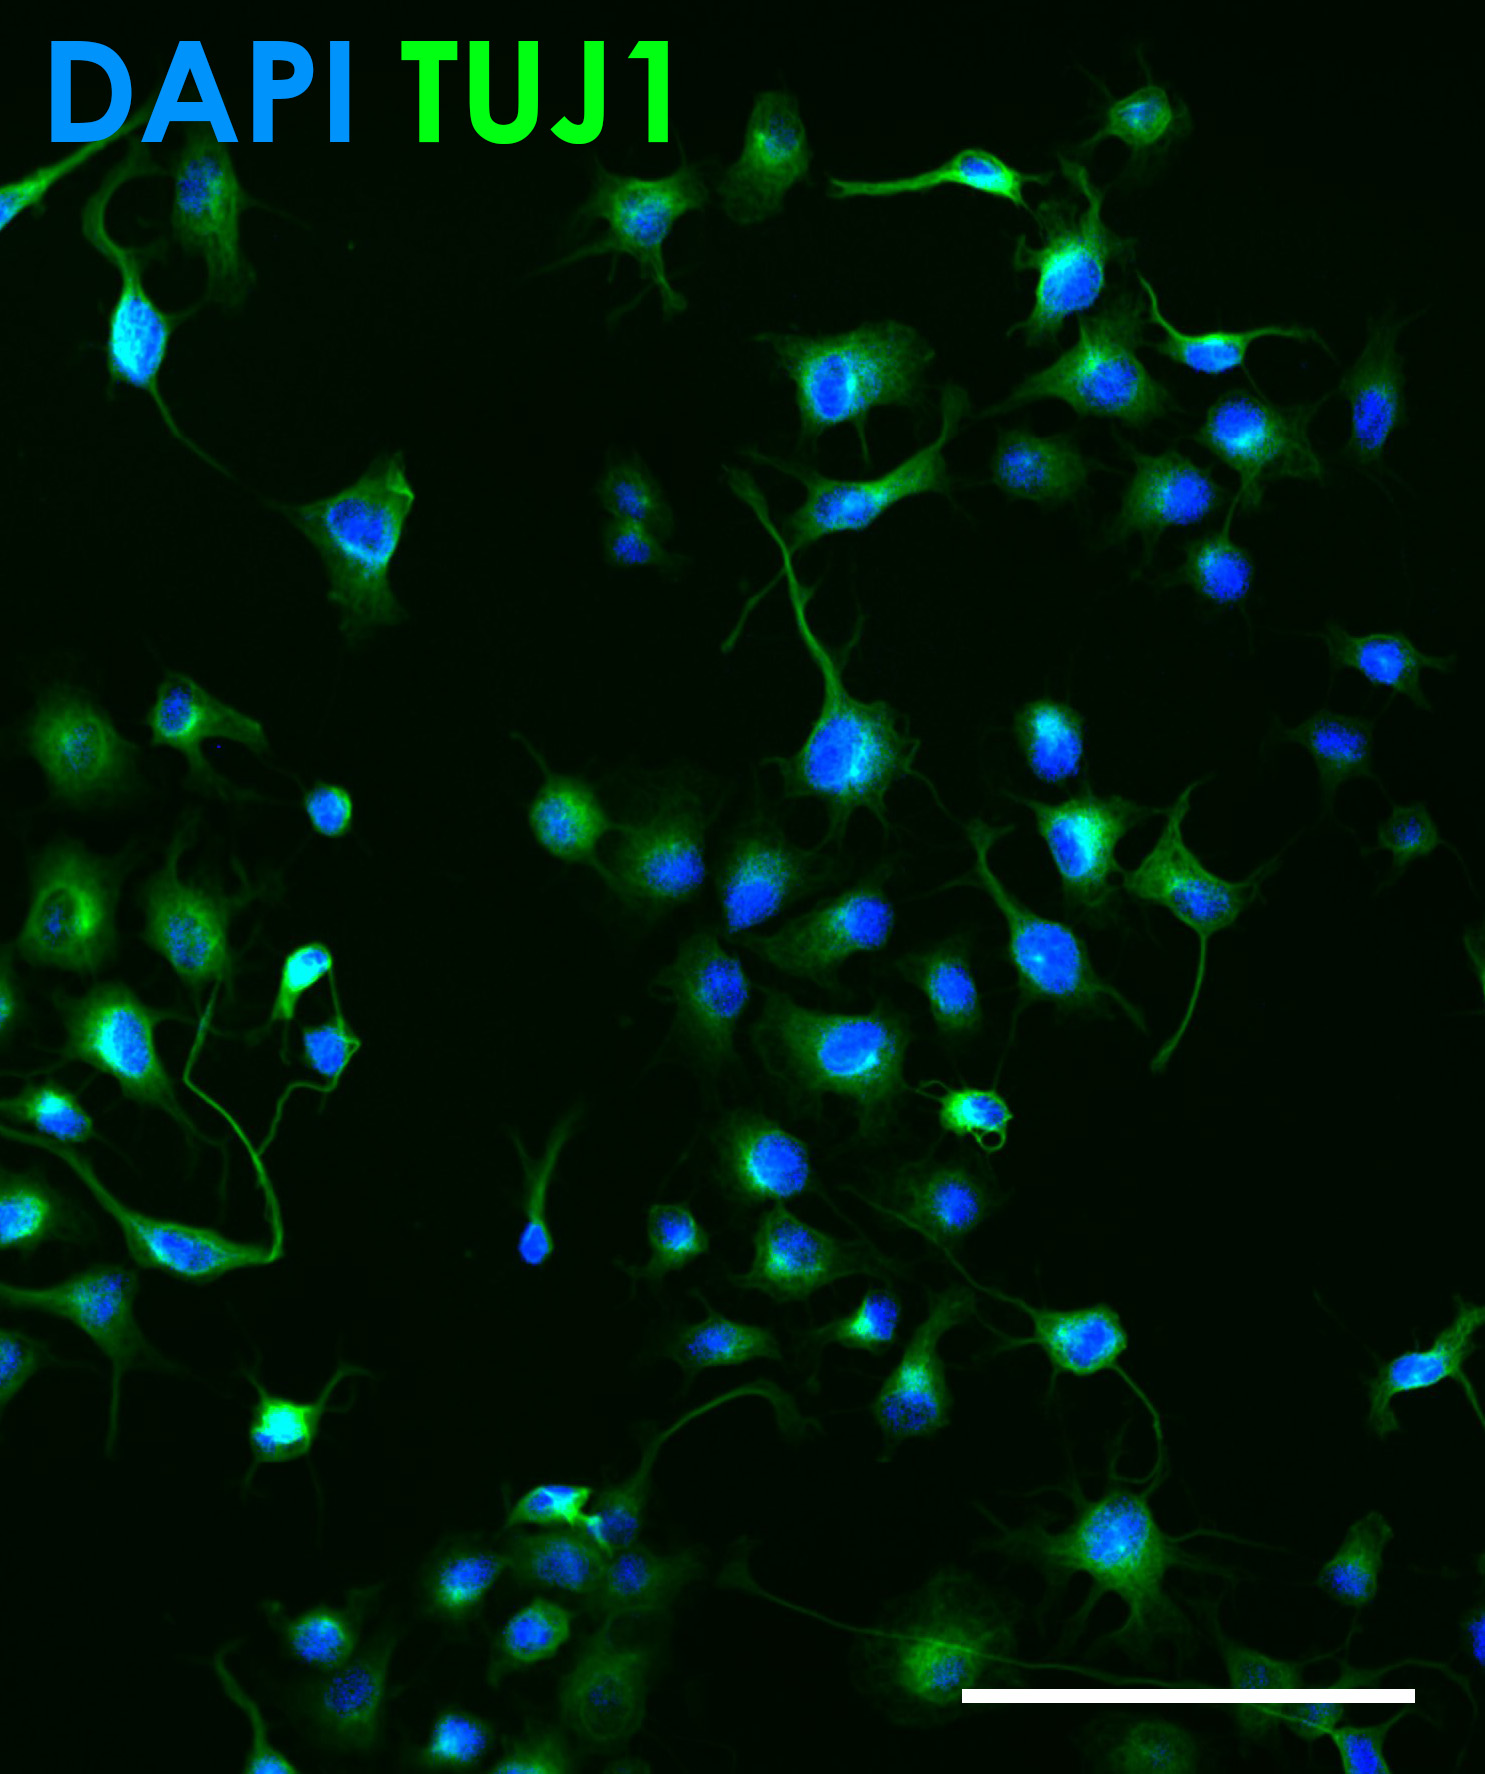
\includegraphics[width=0.196\textwidth]{figures/IF/charac(light)/d0-t}
	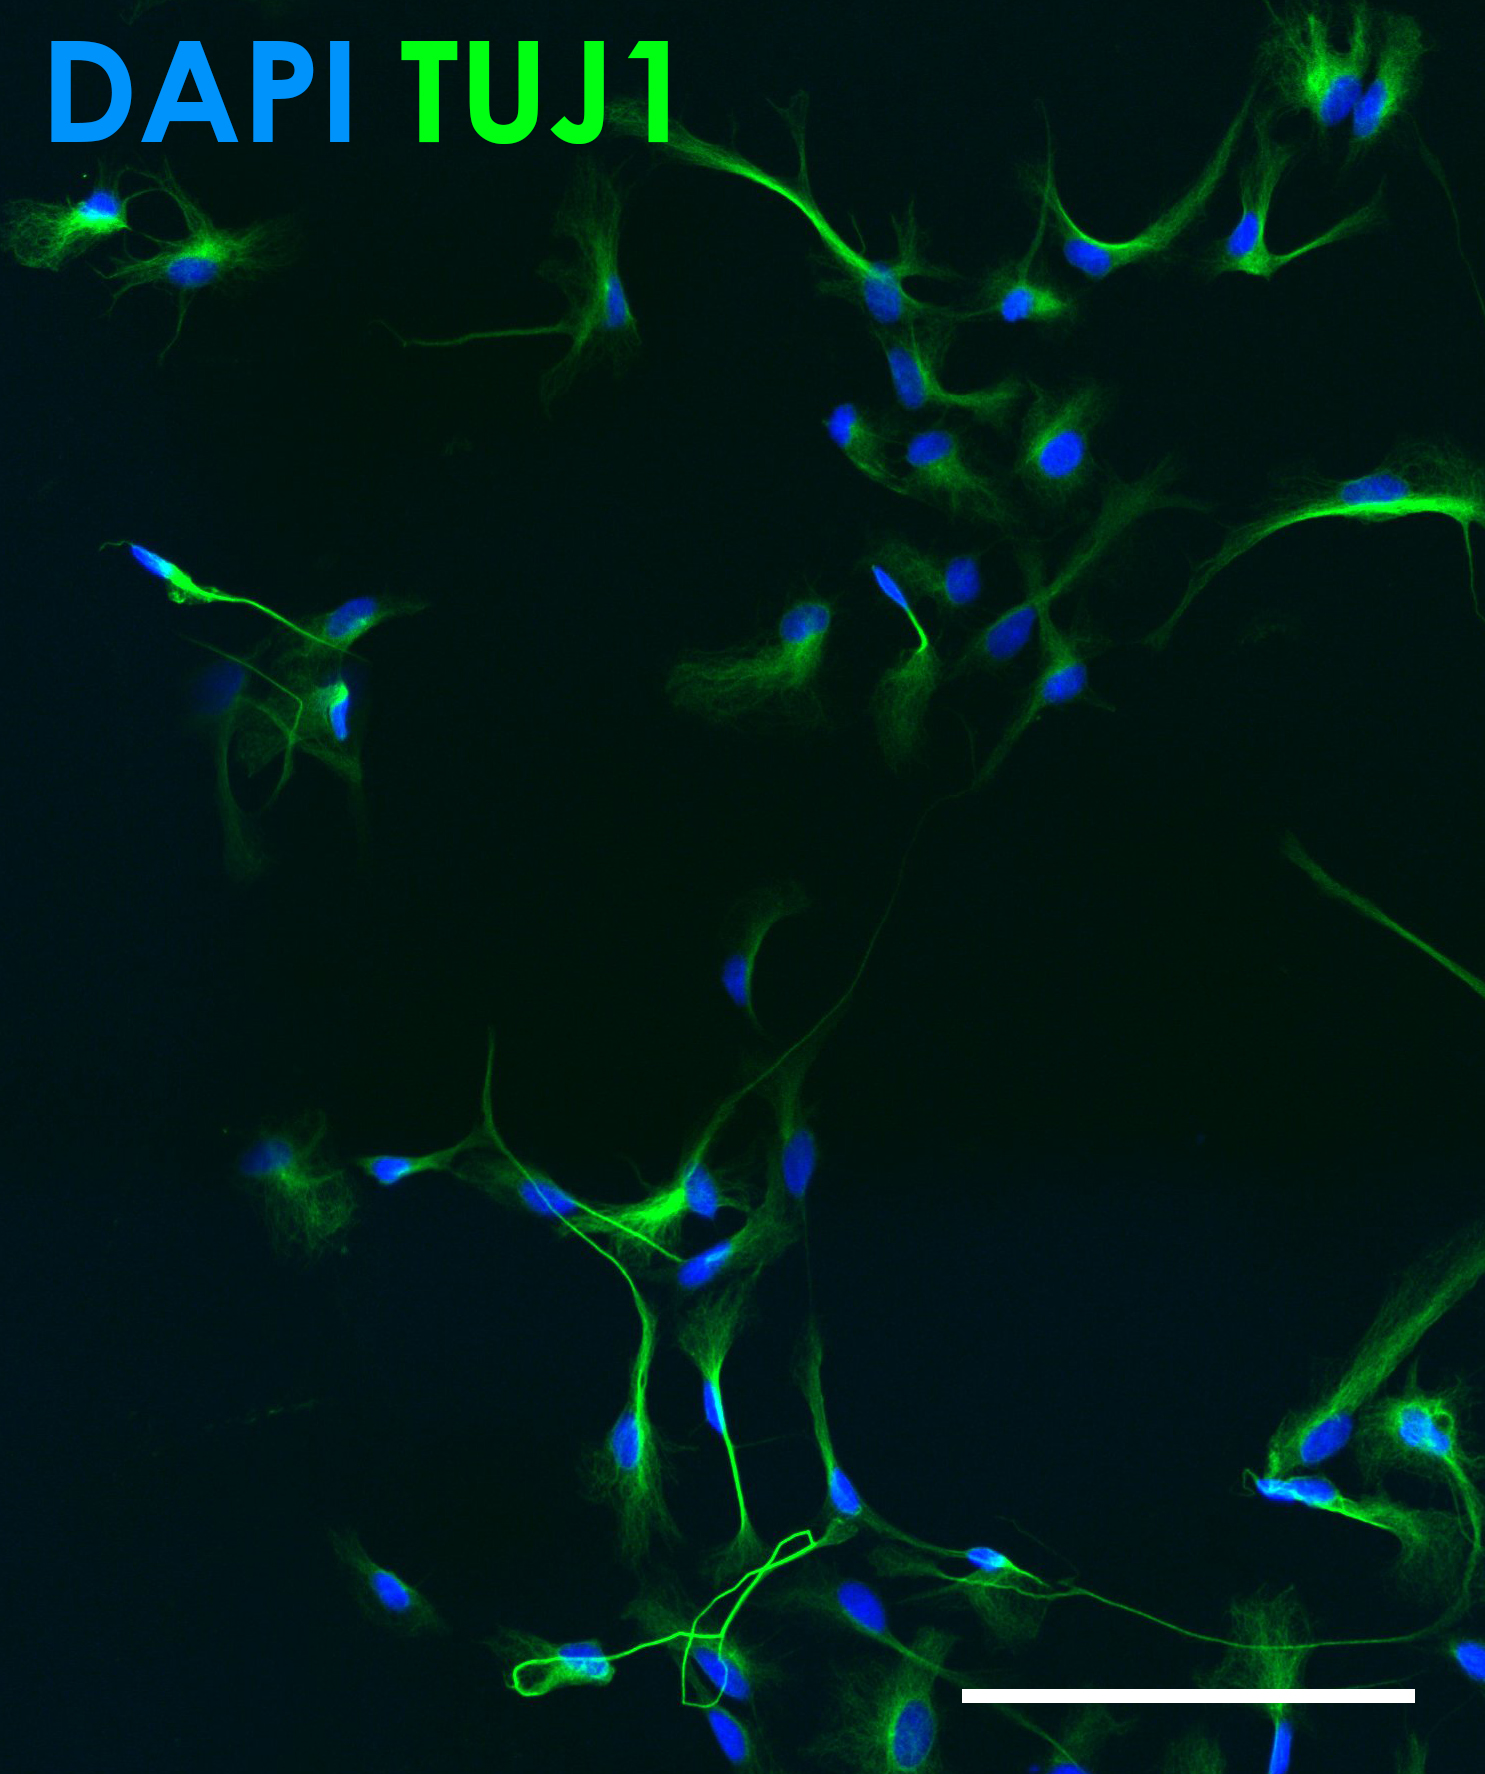
\includegraphics[width=0.196\textwidth]{figures/IF/charac(light)/d3-t}	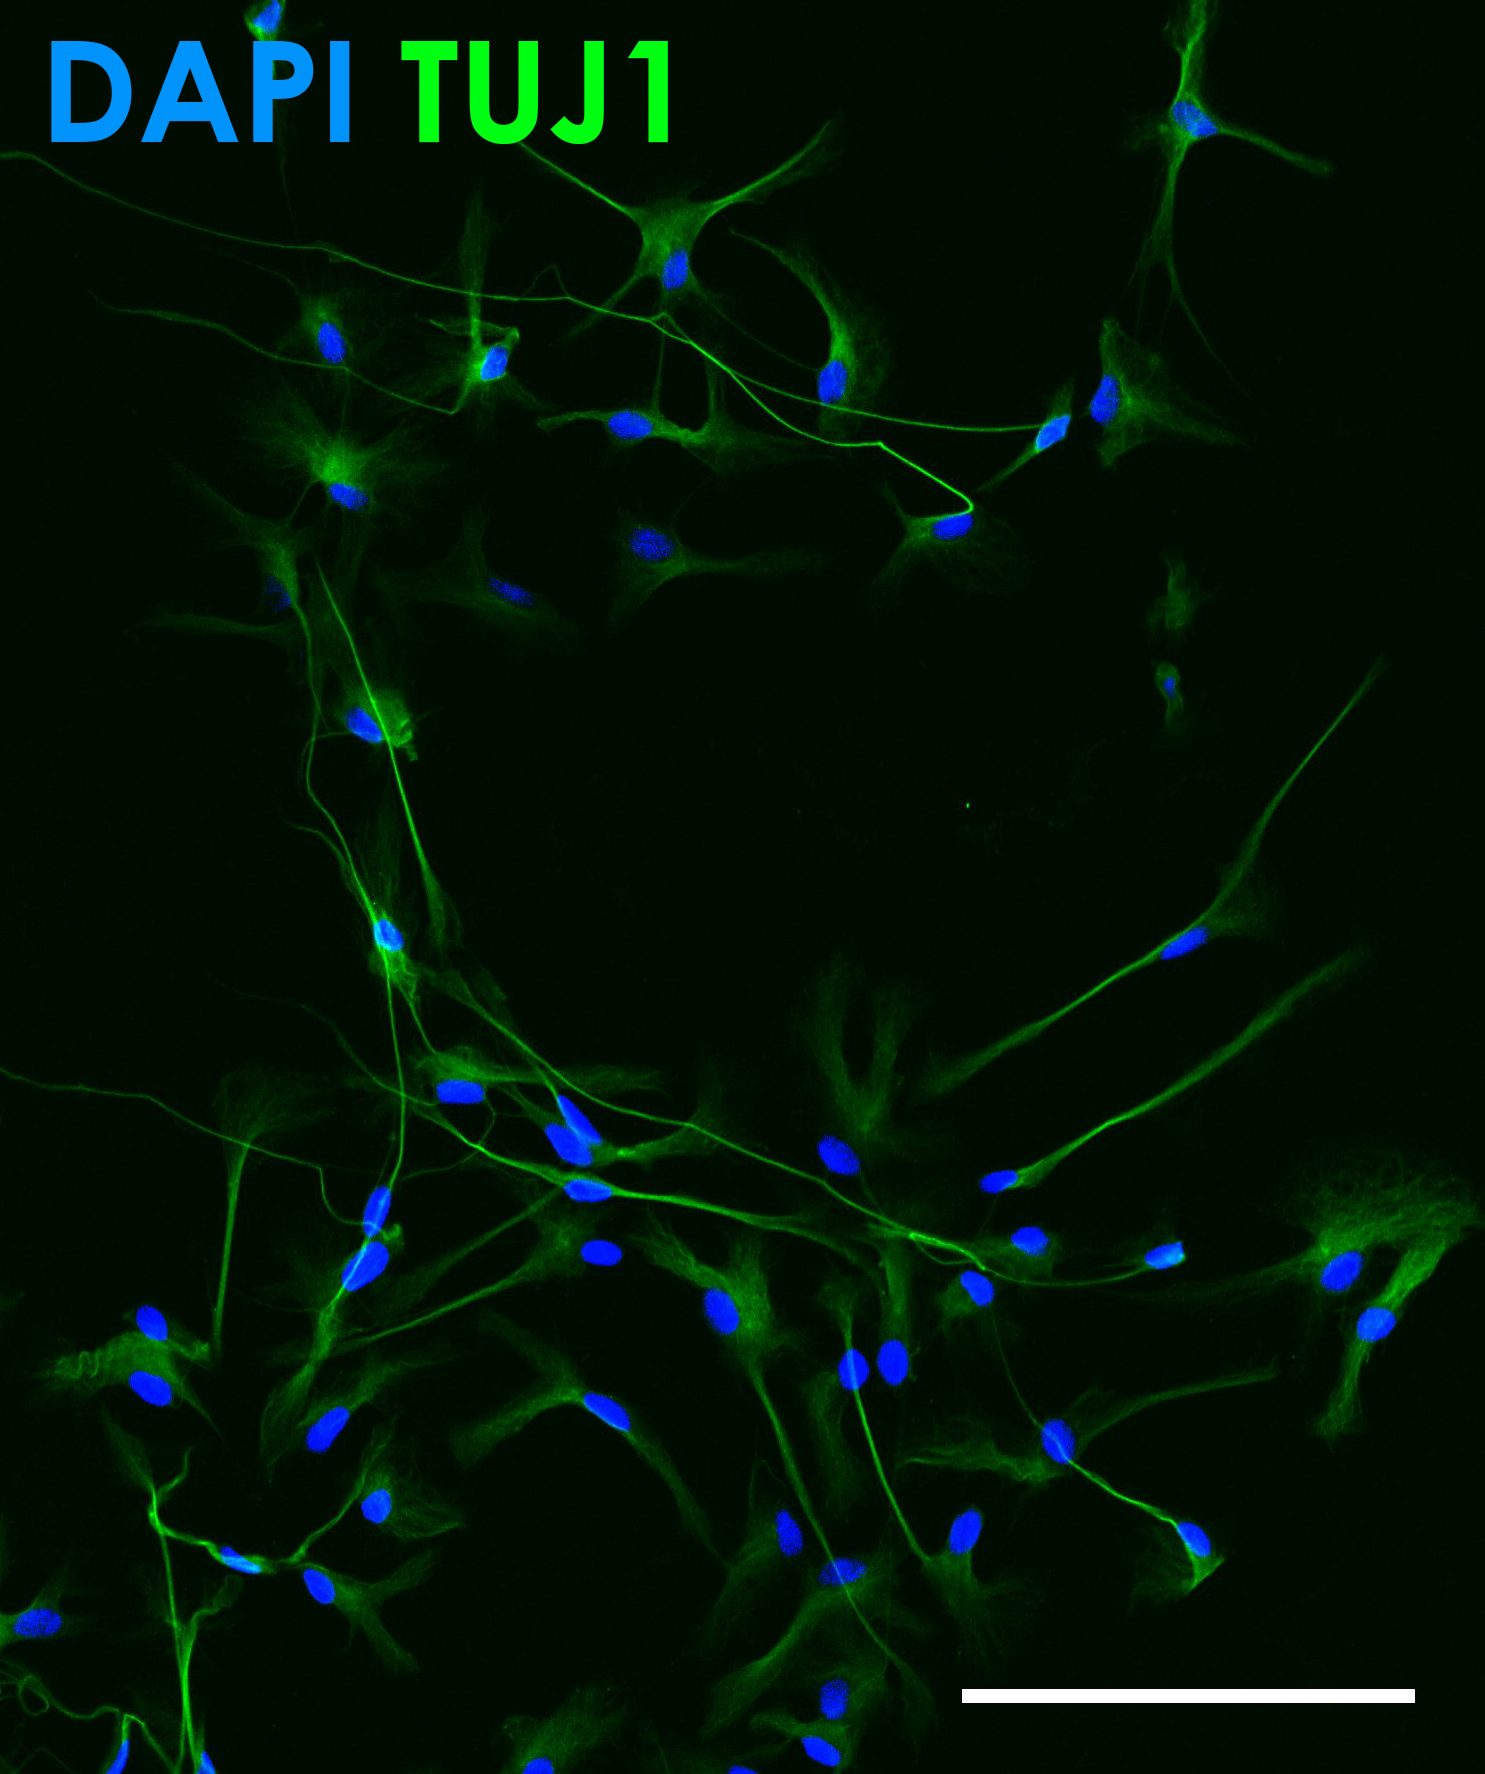
\includegraphics[width=0.196\textwidth]{figures/IF/charac(light)/d7-t}	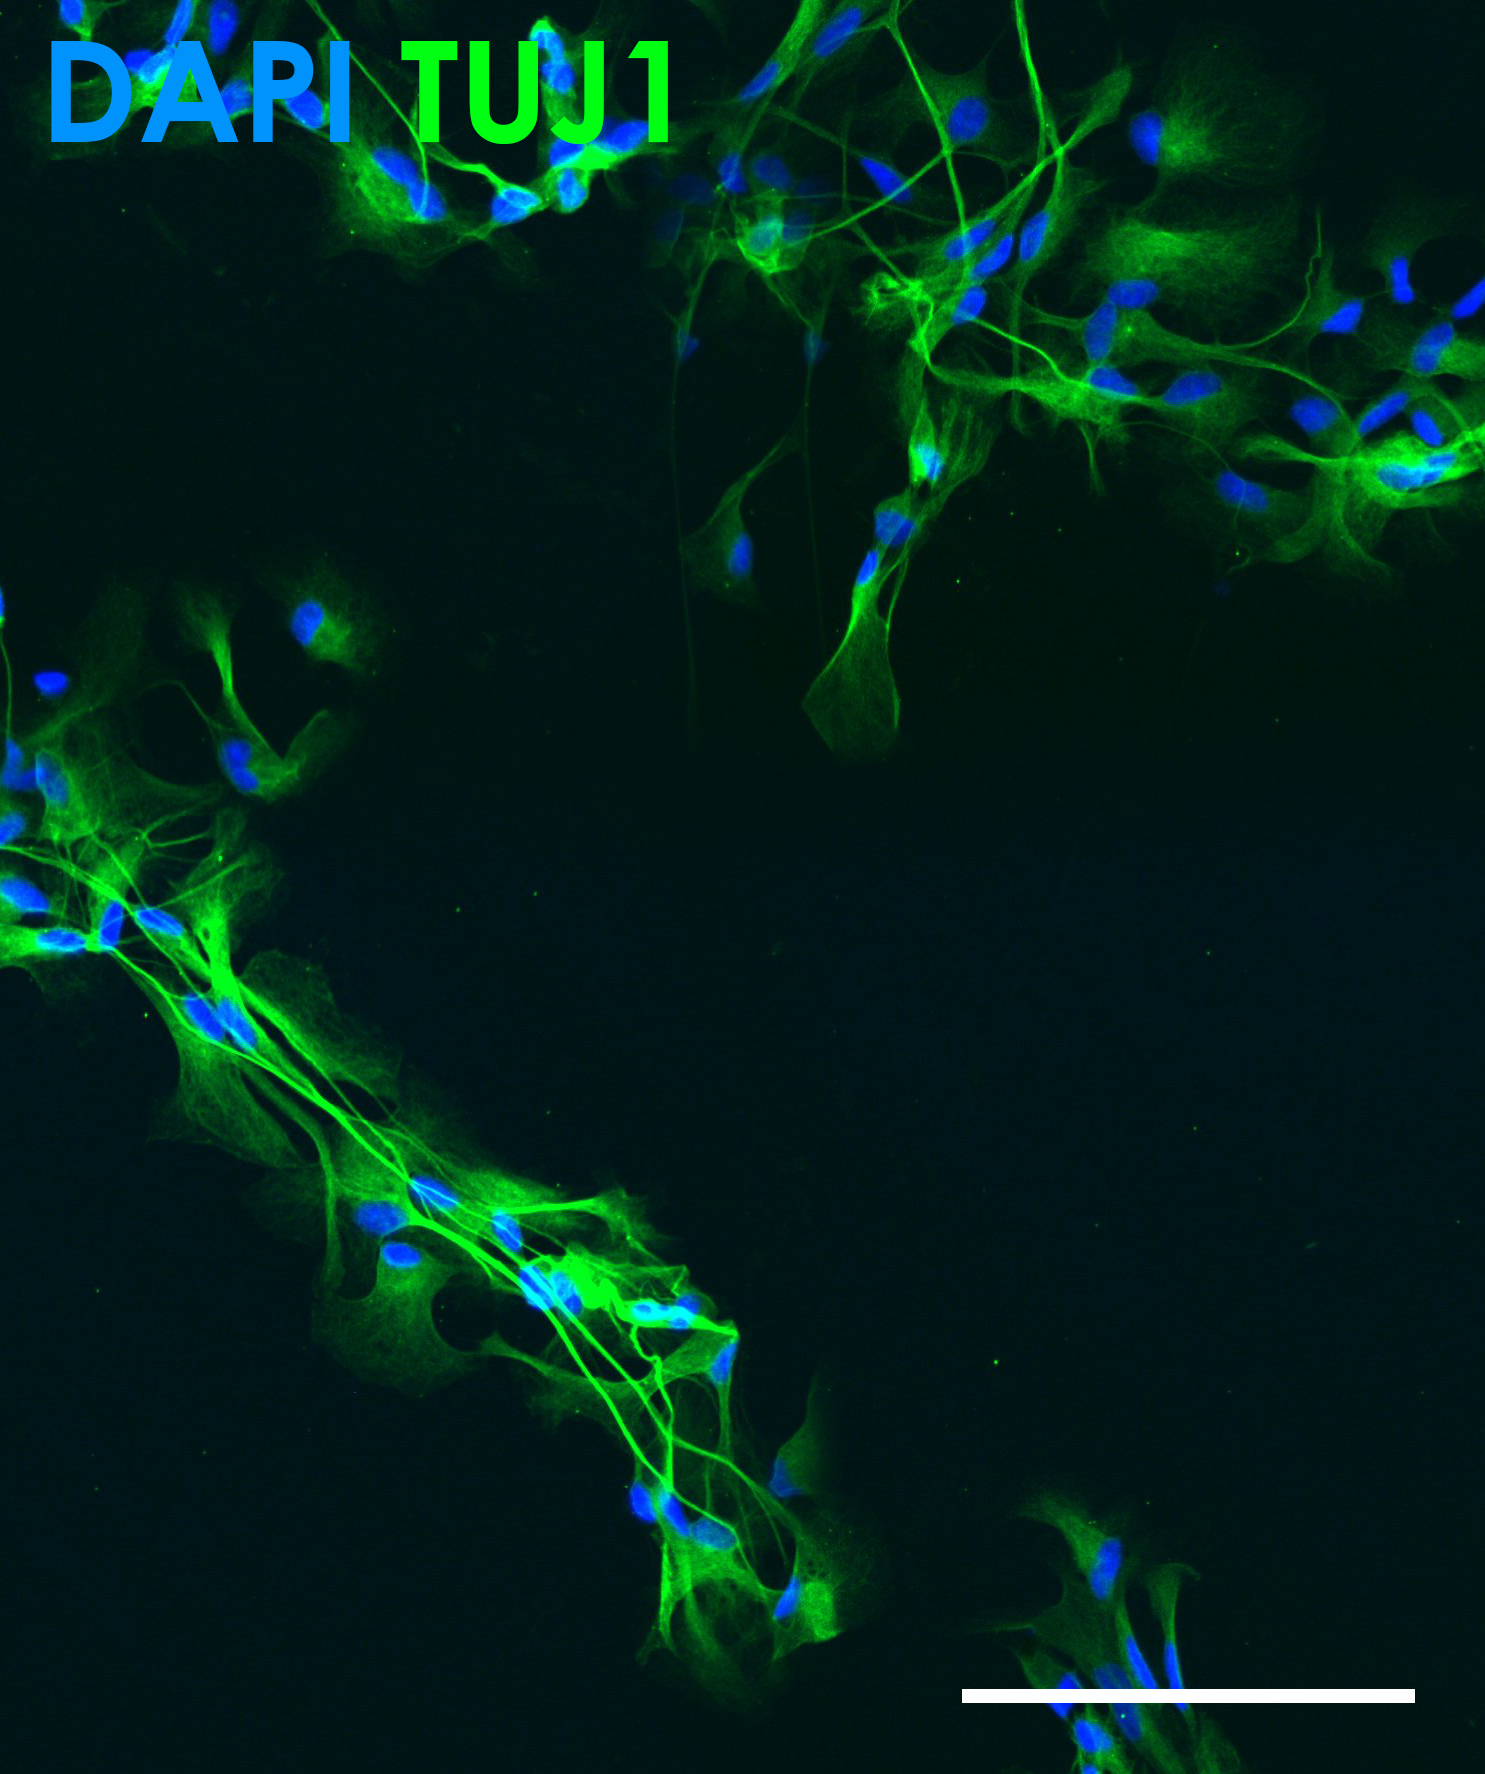
\includegraphics[width=0.196\textwidth]{figures/IF/charac(light)/d14-t}	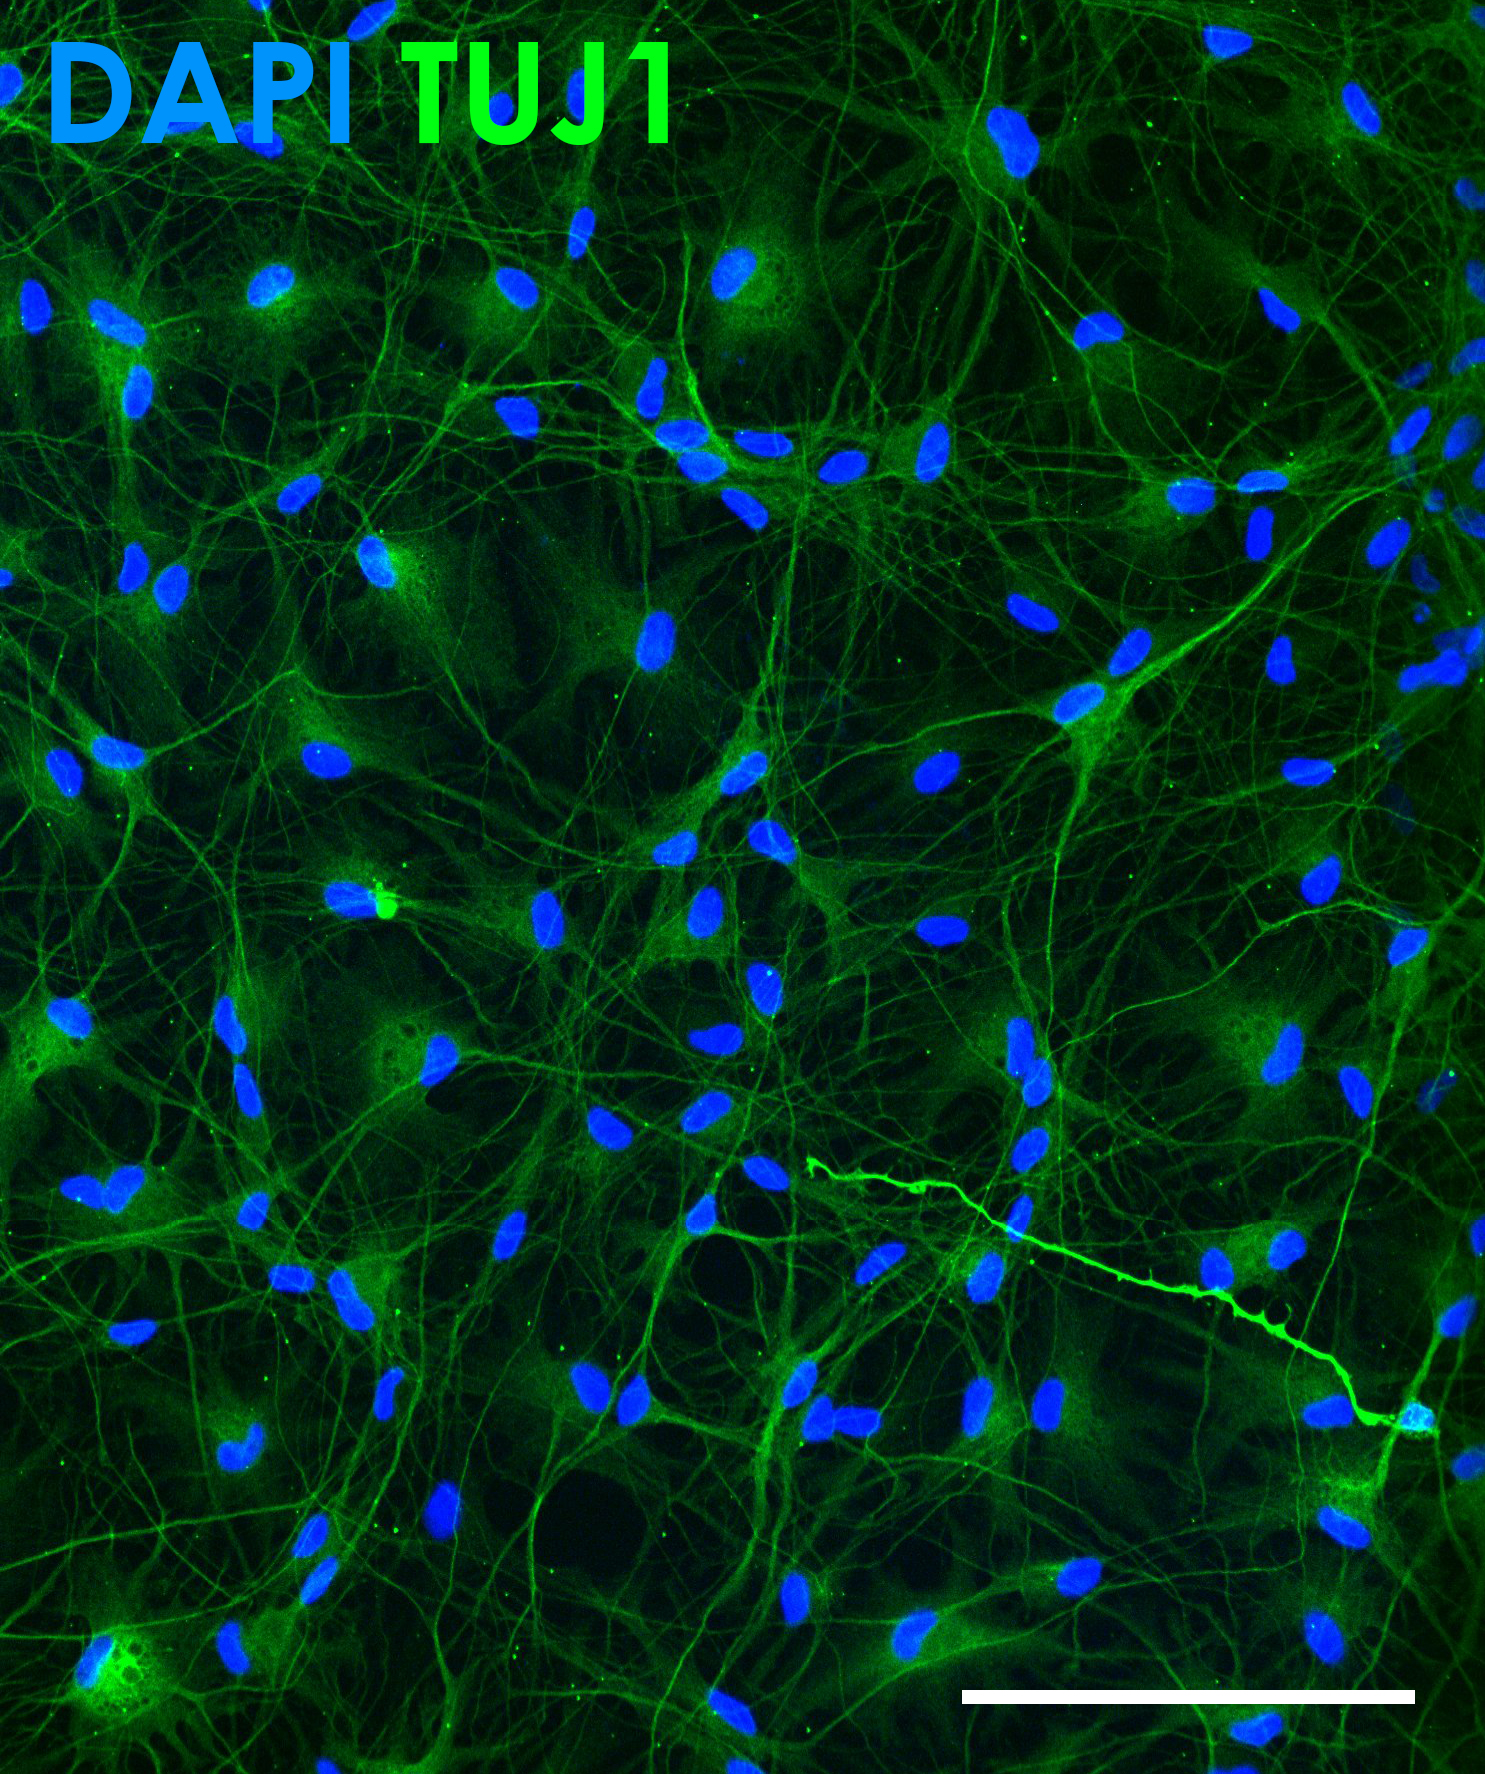
\includegraphics[width=0.196\textwidth]{figures/IF/charac(light)/d21-t}
	
	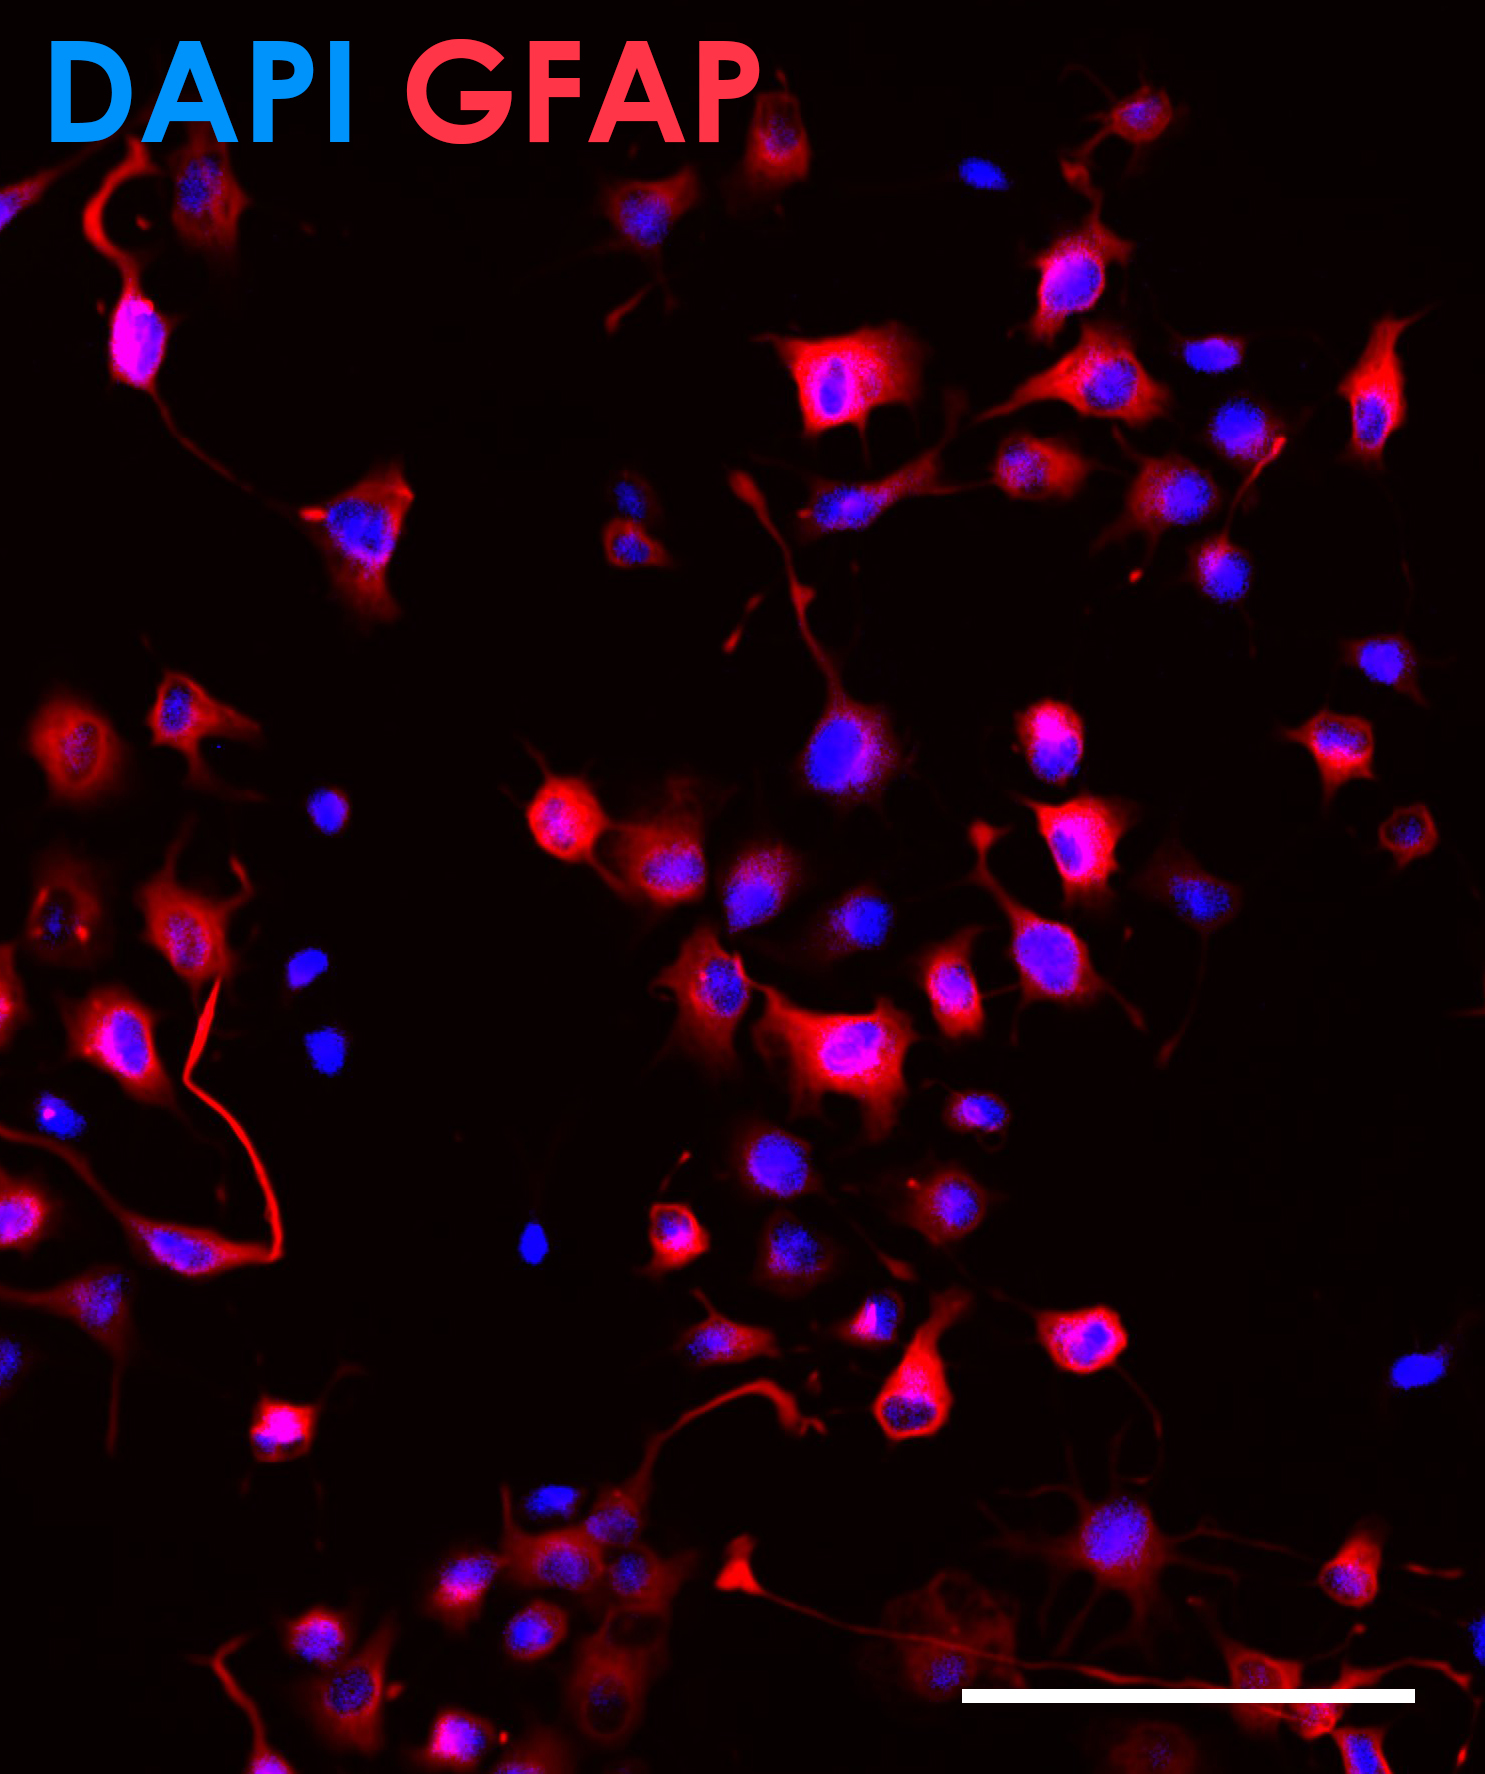
\includegraphics[width=0.196\textwidth]{figures/IF/charac(light)/d0-g}
	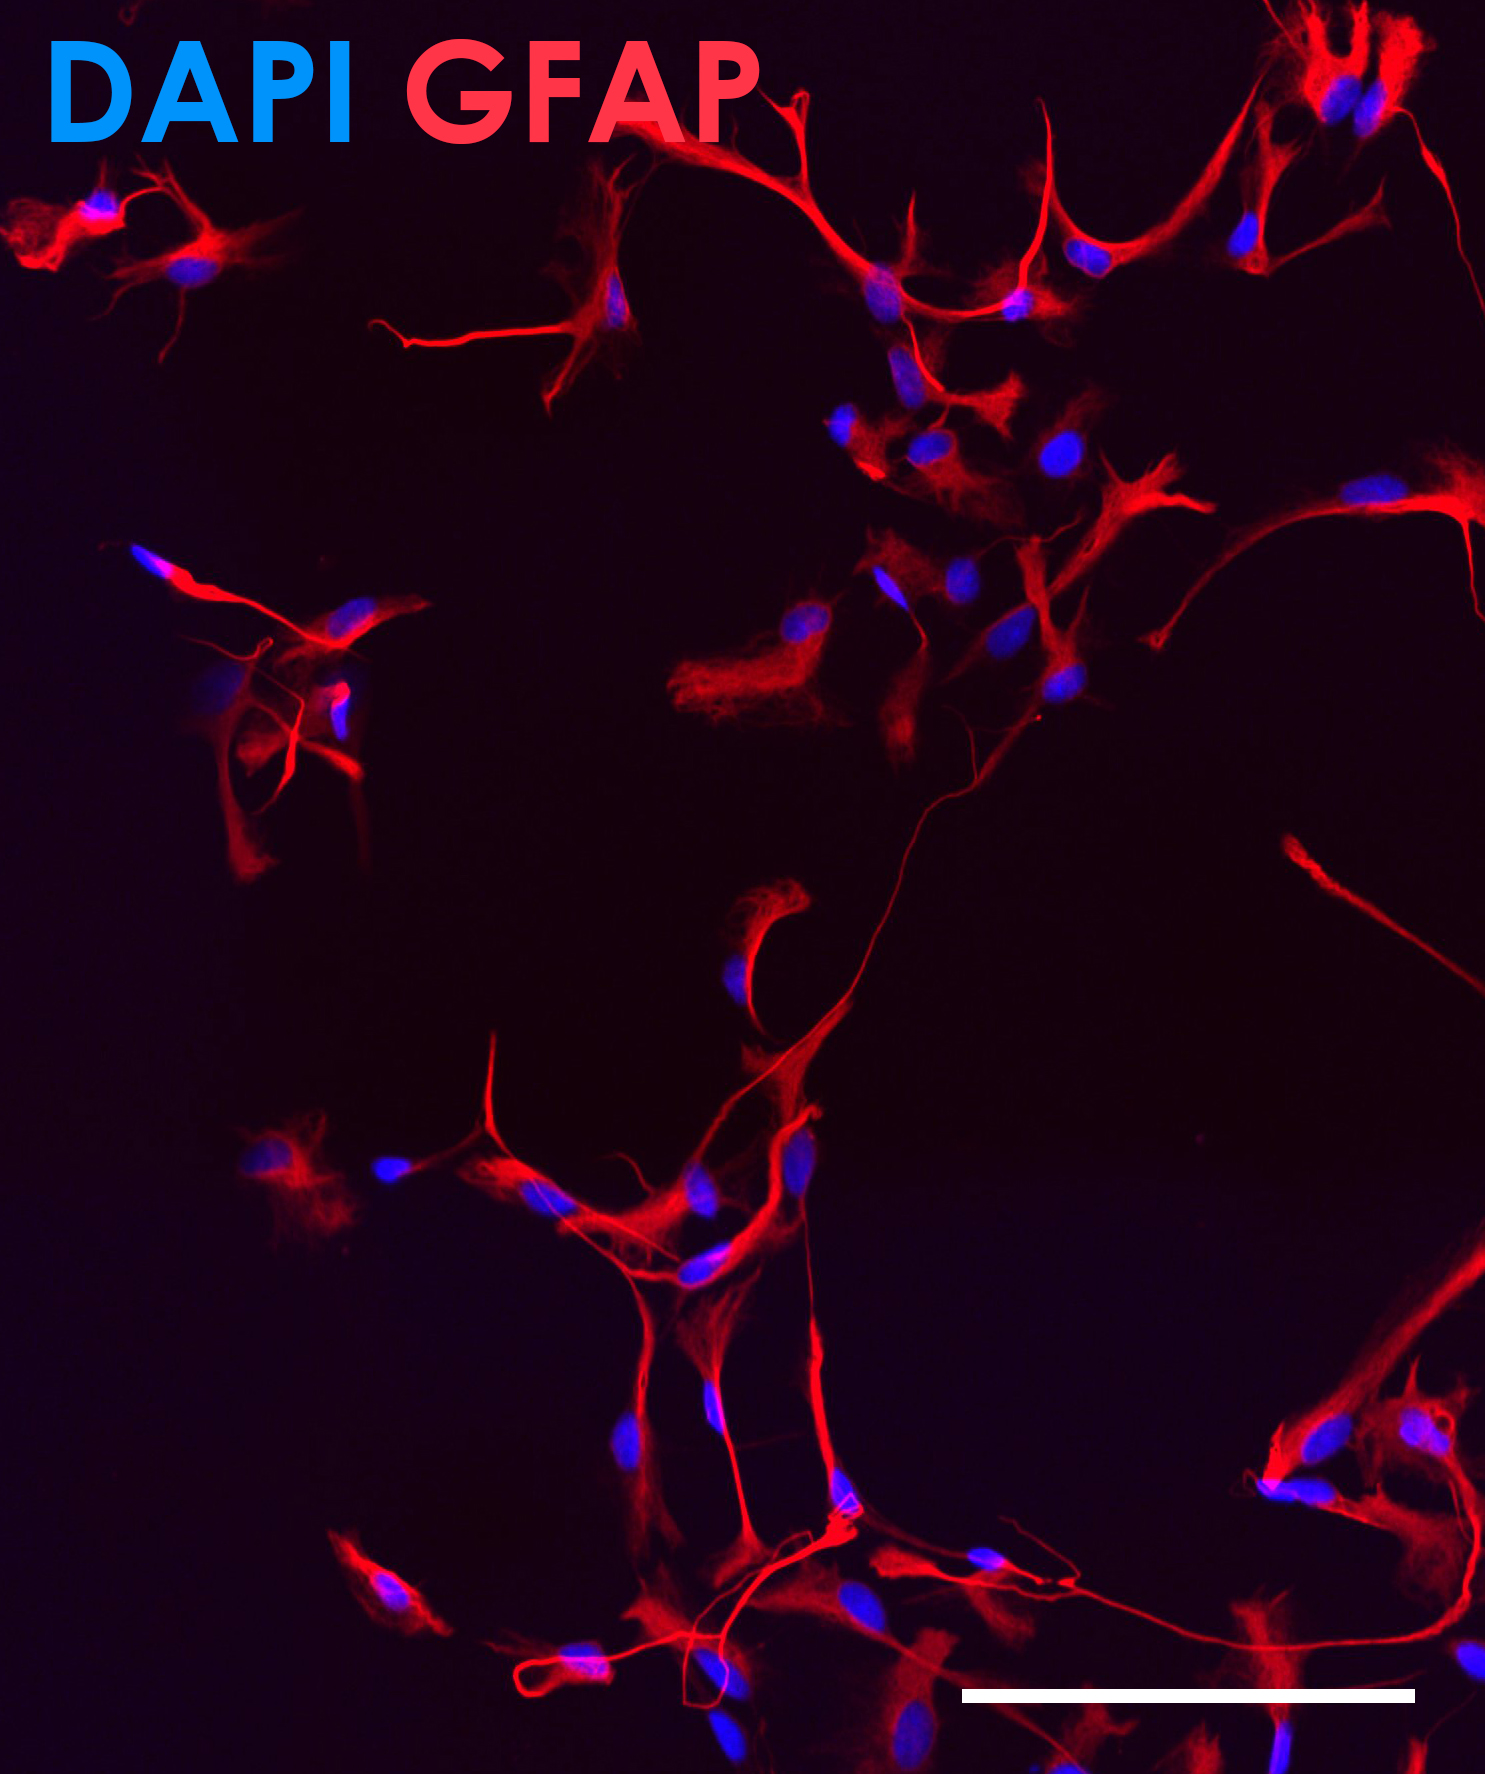
\includegraphics[width=0.196\textwidth]{figures/IF/charac(light)/d3-g}	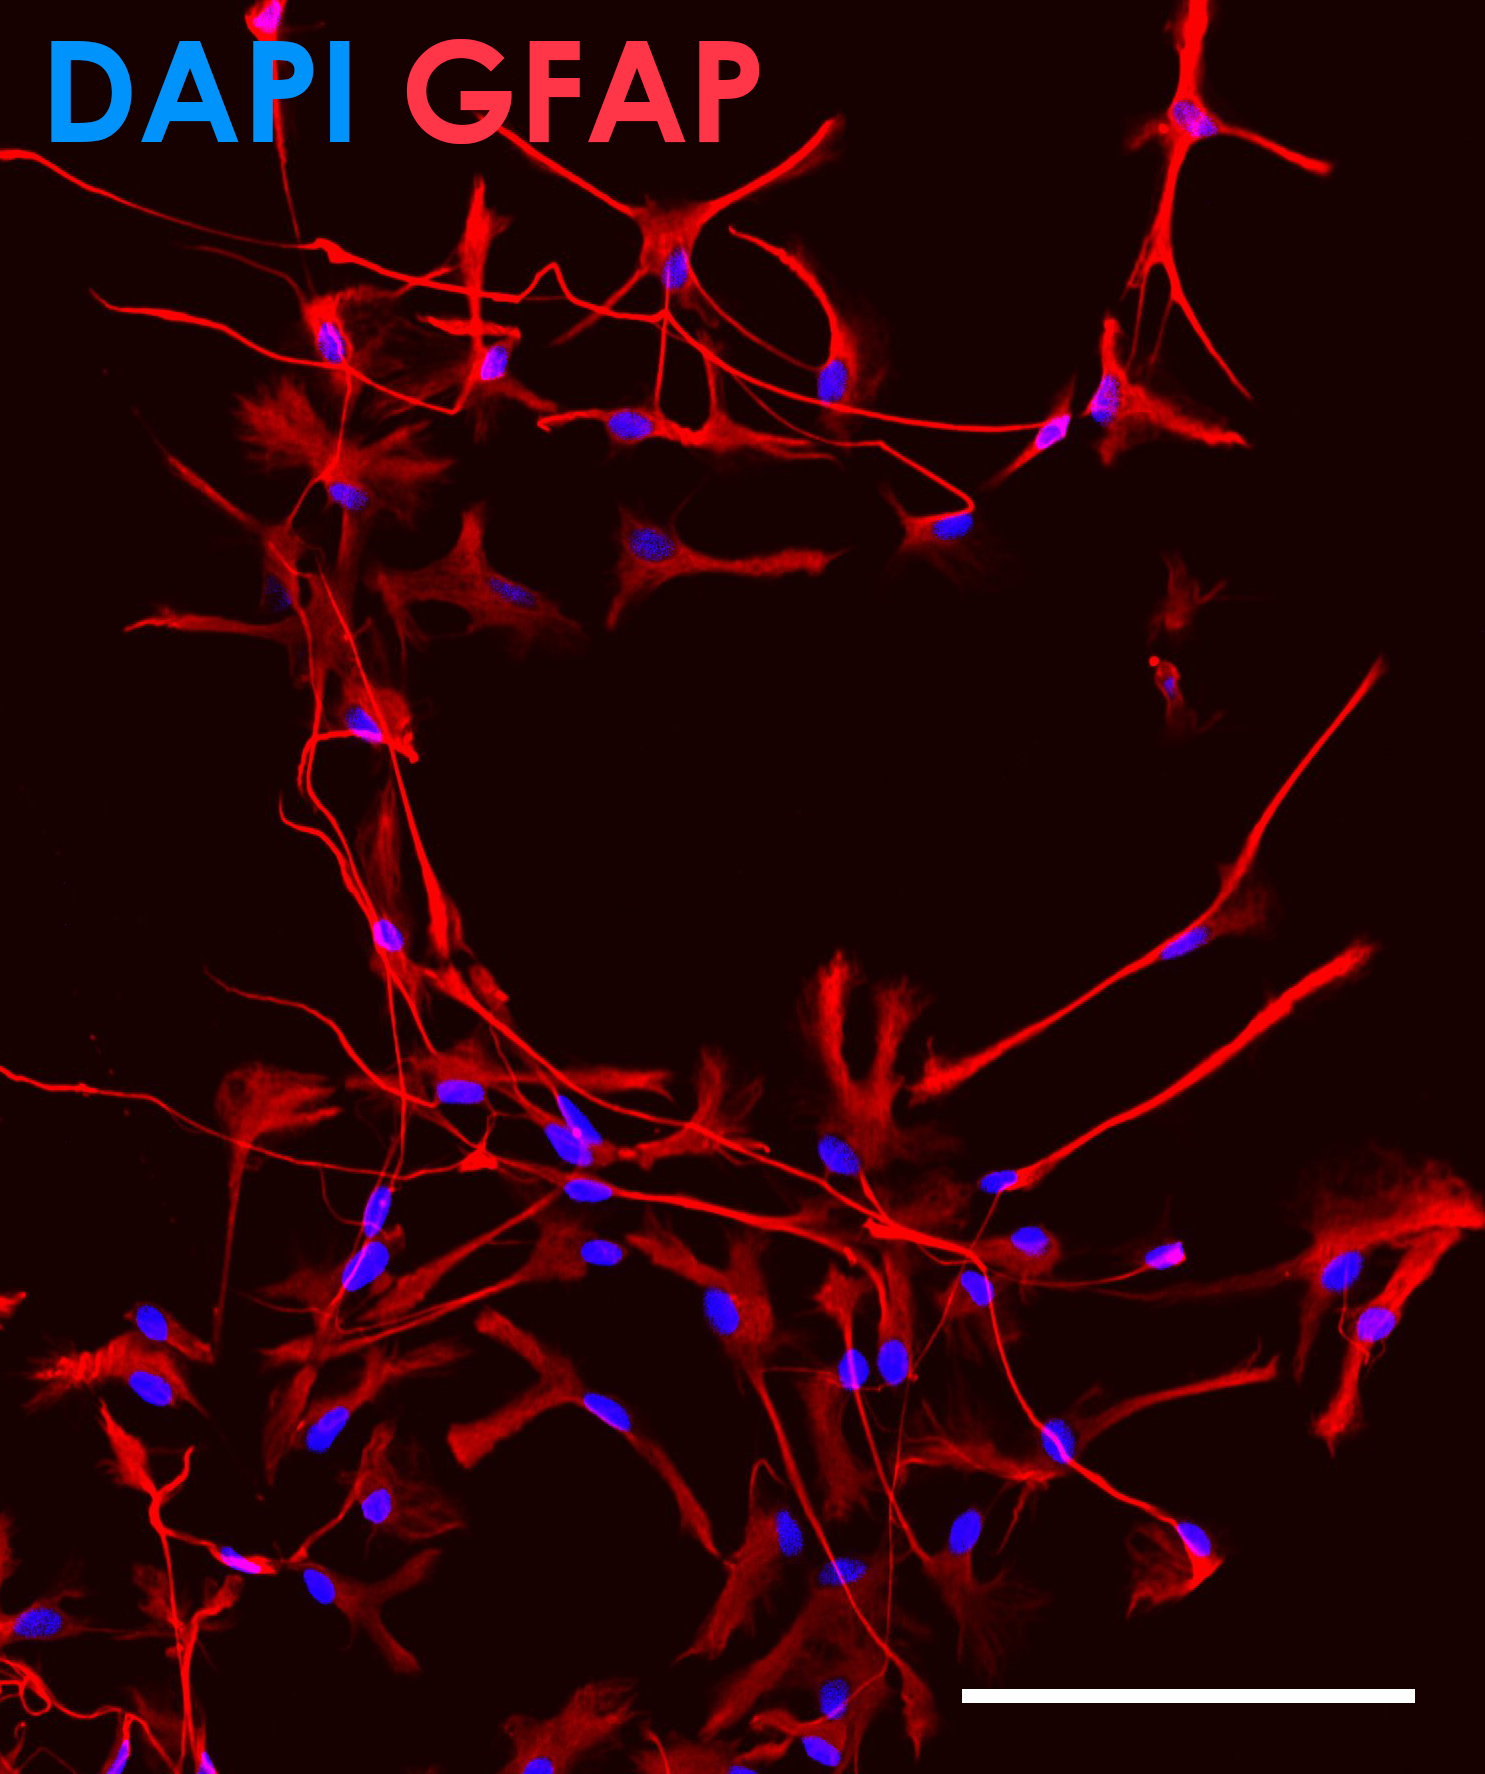
\includegraphics[width=0.196\textwidth]{figures/IF/charac(light)/d7-g}	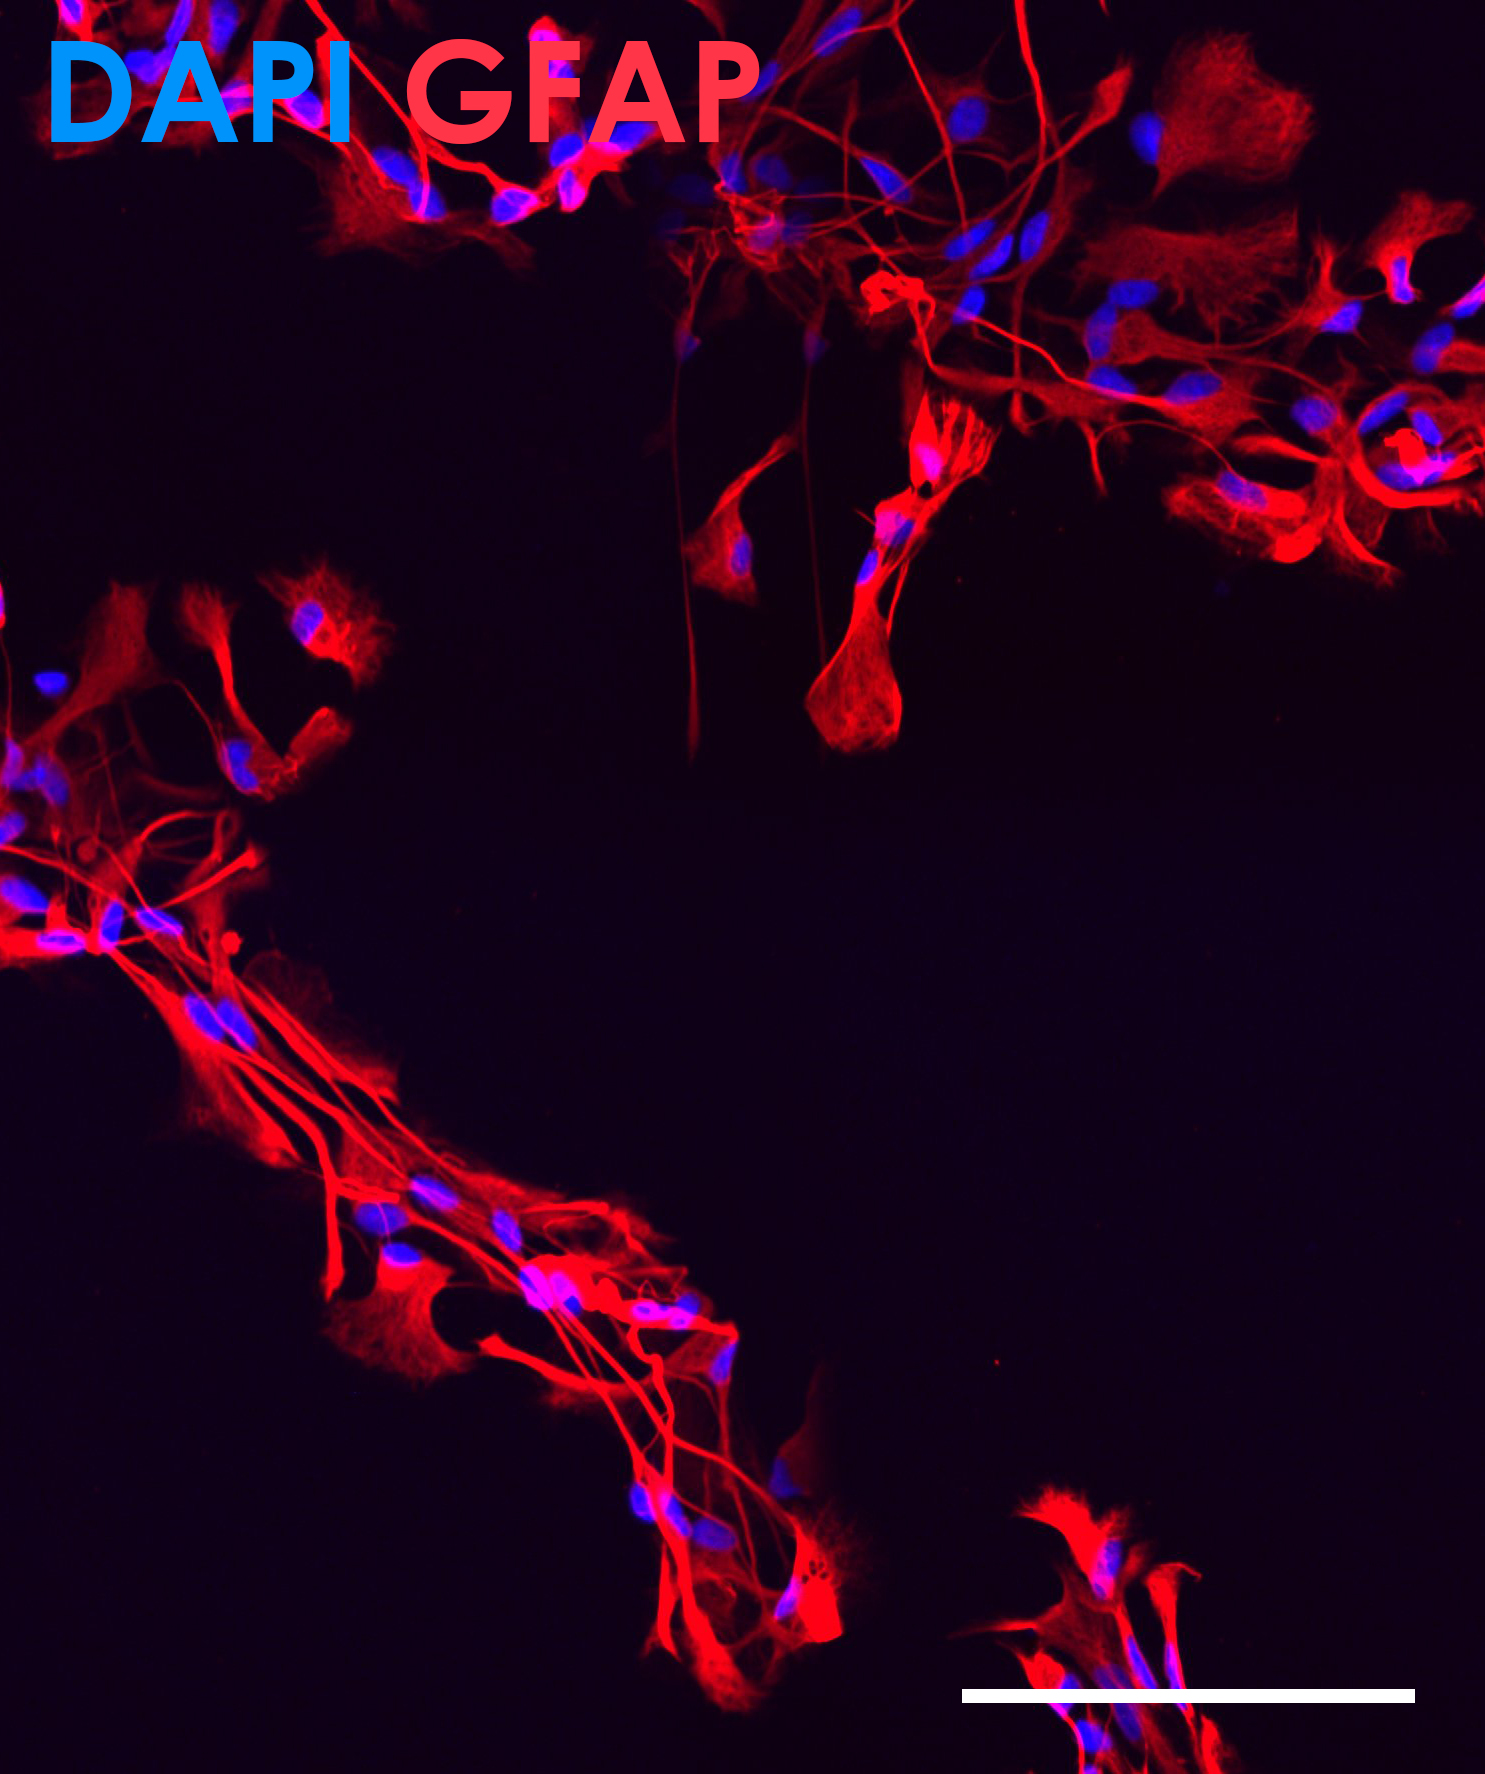
\includegraphics[width=0.196\textwidth]{figures/IF/charac(light)/d14-g}	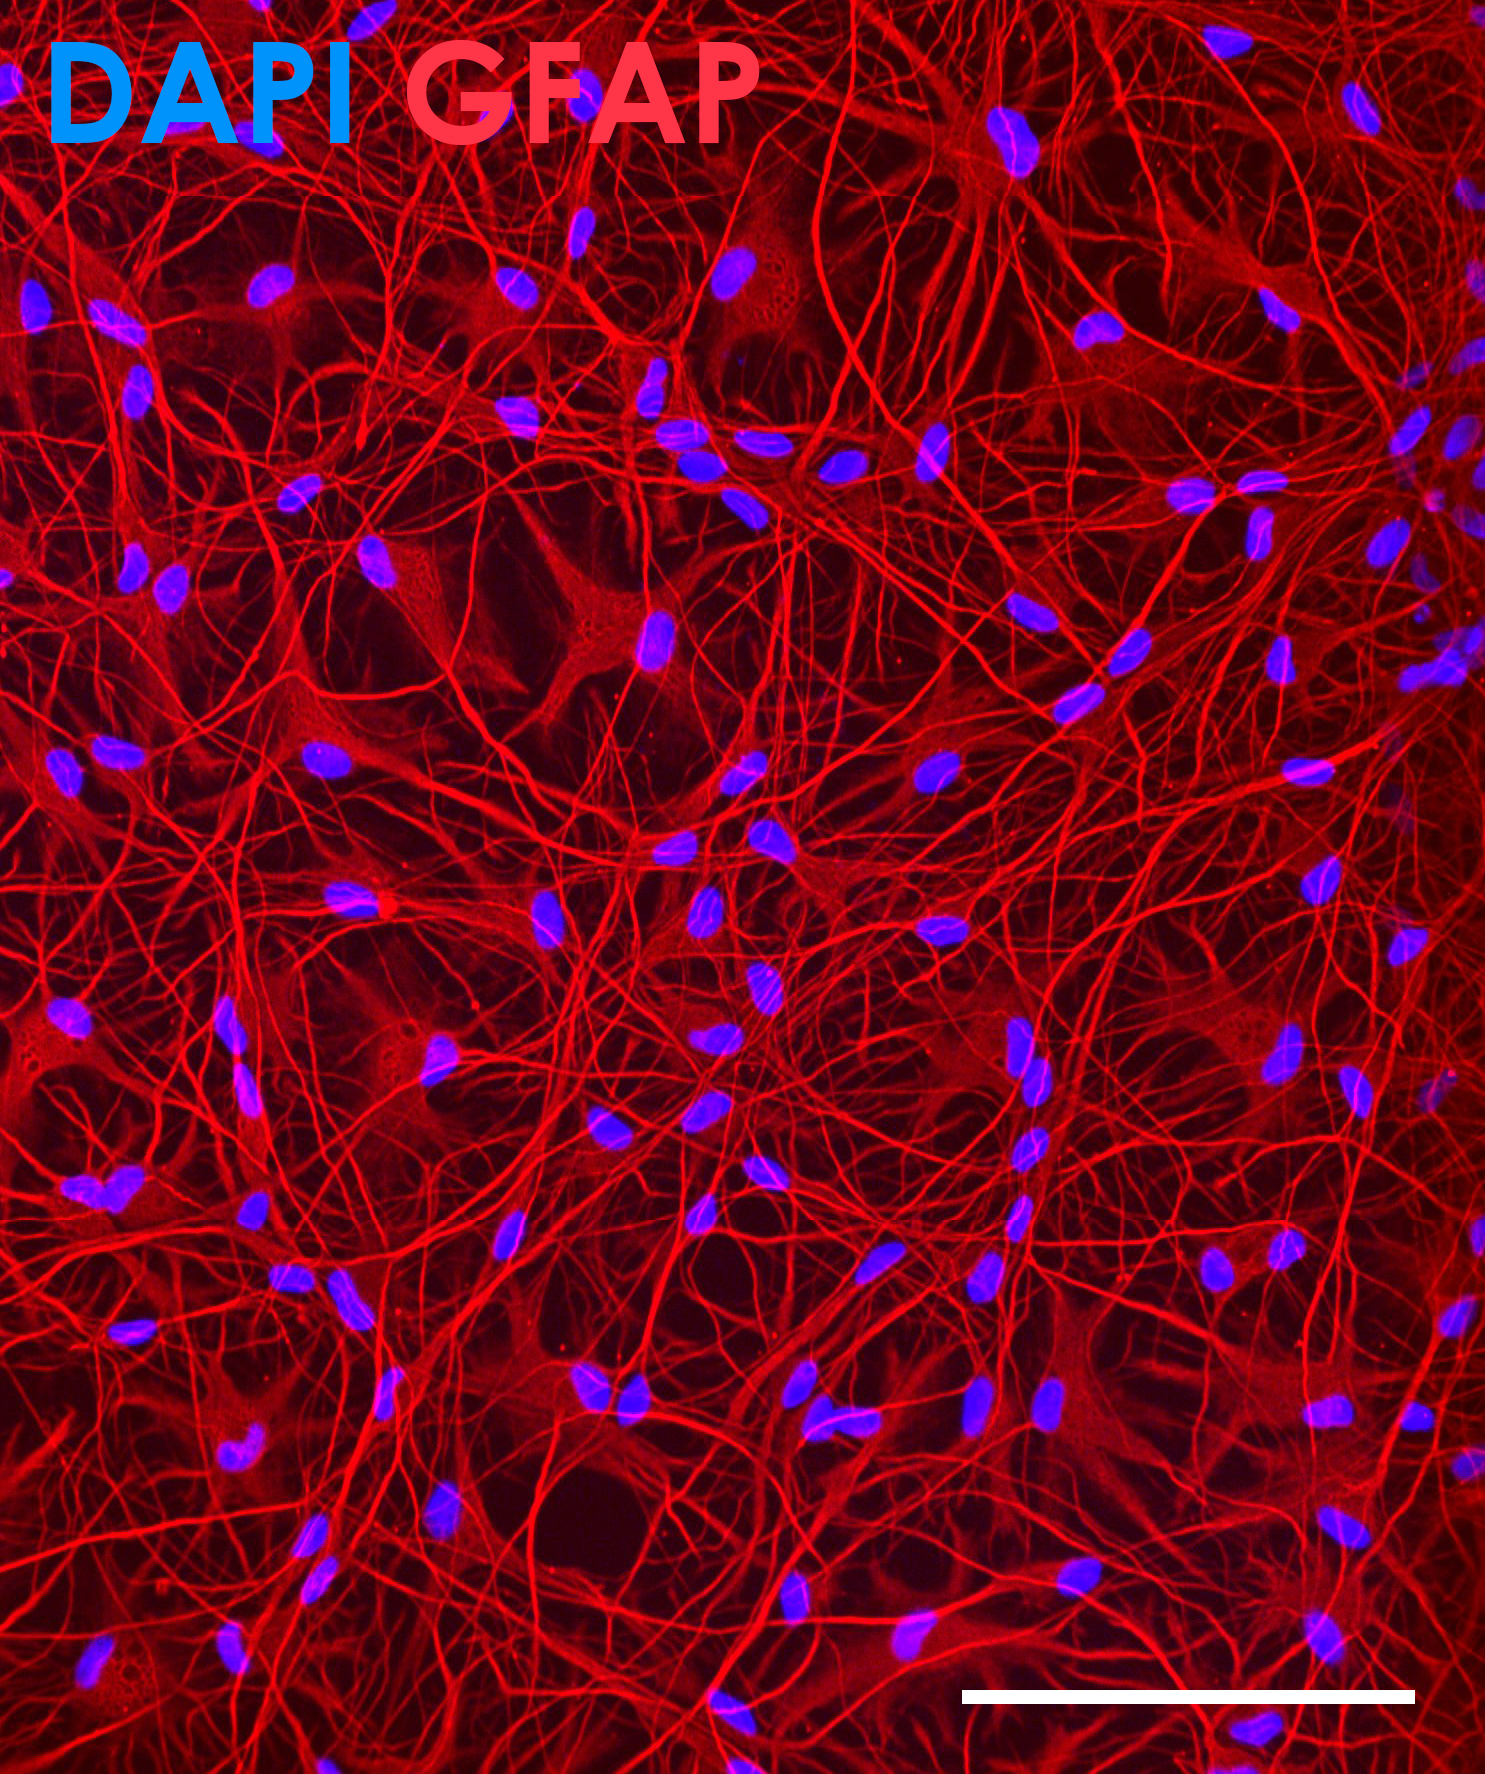
\includegraphics[width=0.196\textwidth]{figures/IF/charac(light)/d21-g}
	
	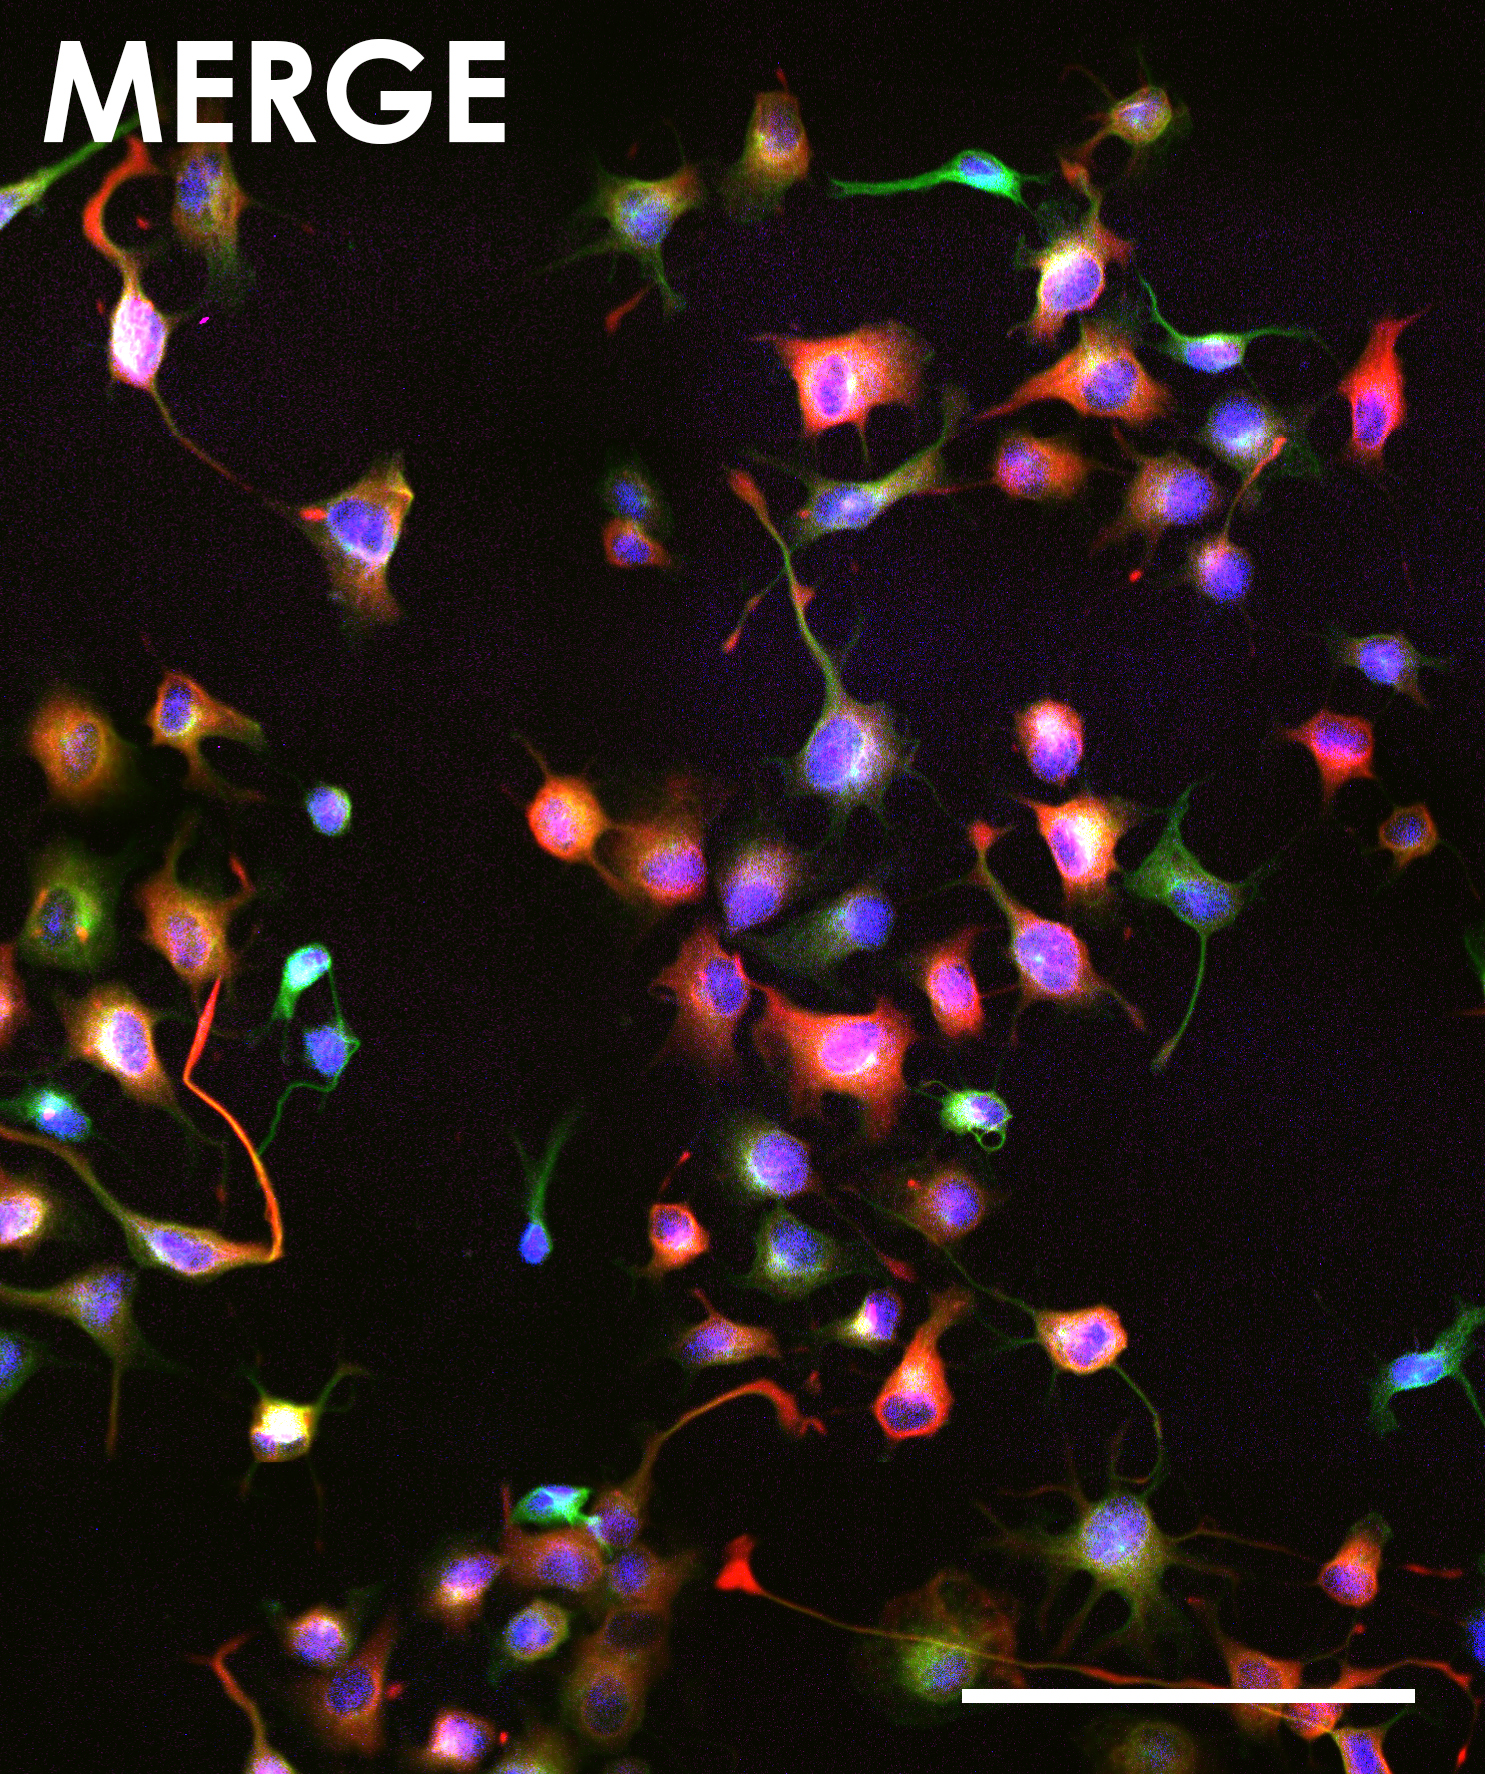
\includegraphics[width=0.196\textwidth]{figures/IF/charac(light)/d0-m}
	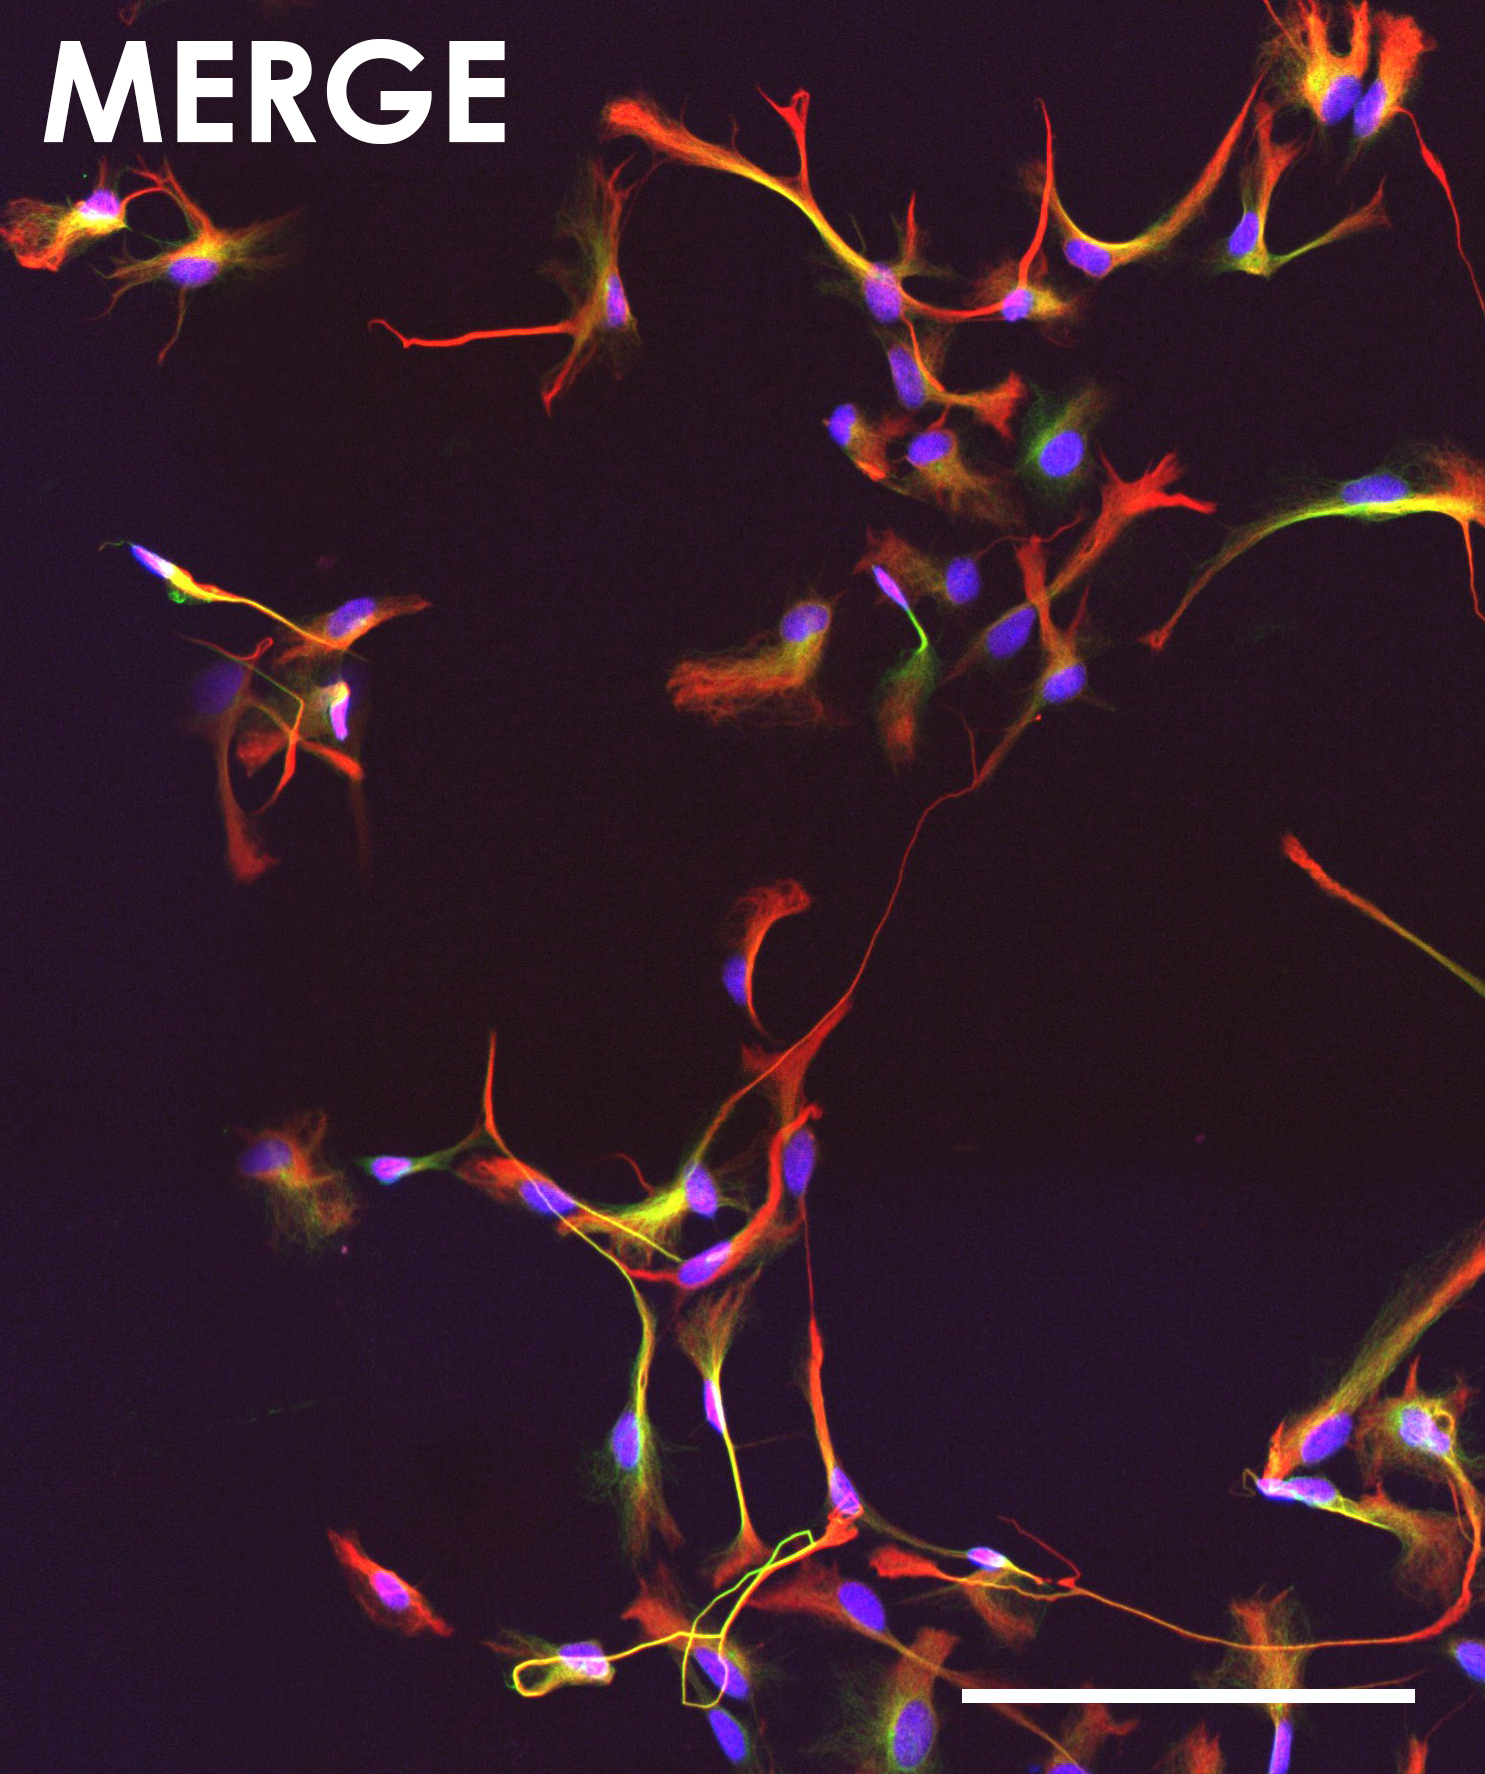
\includegraphics[width=0.196\textwidth]{figures/IF/charac(light)/d3-m}	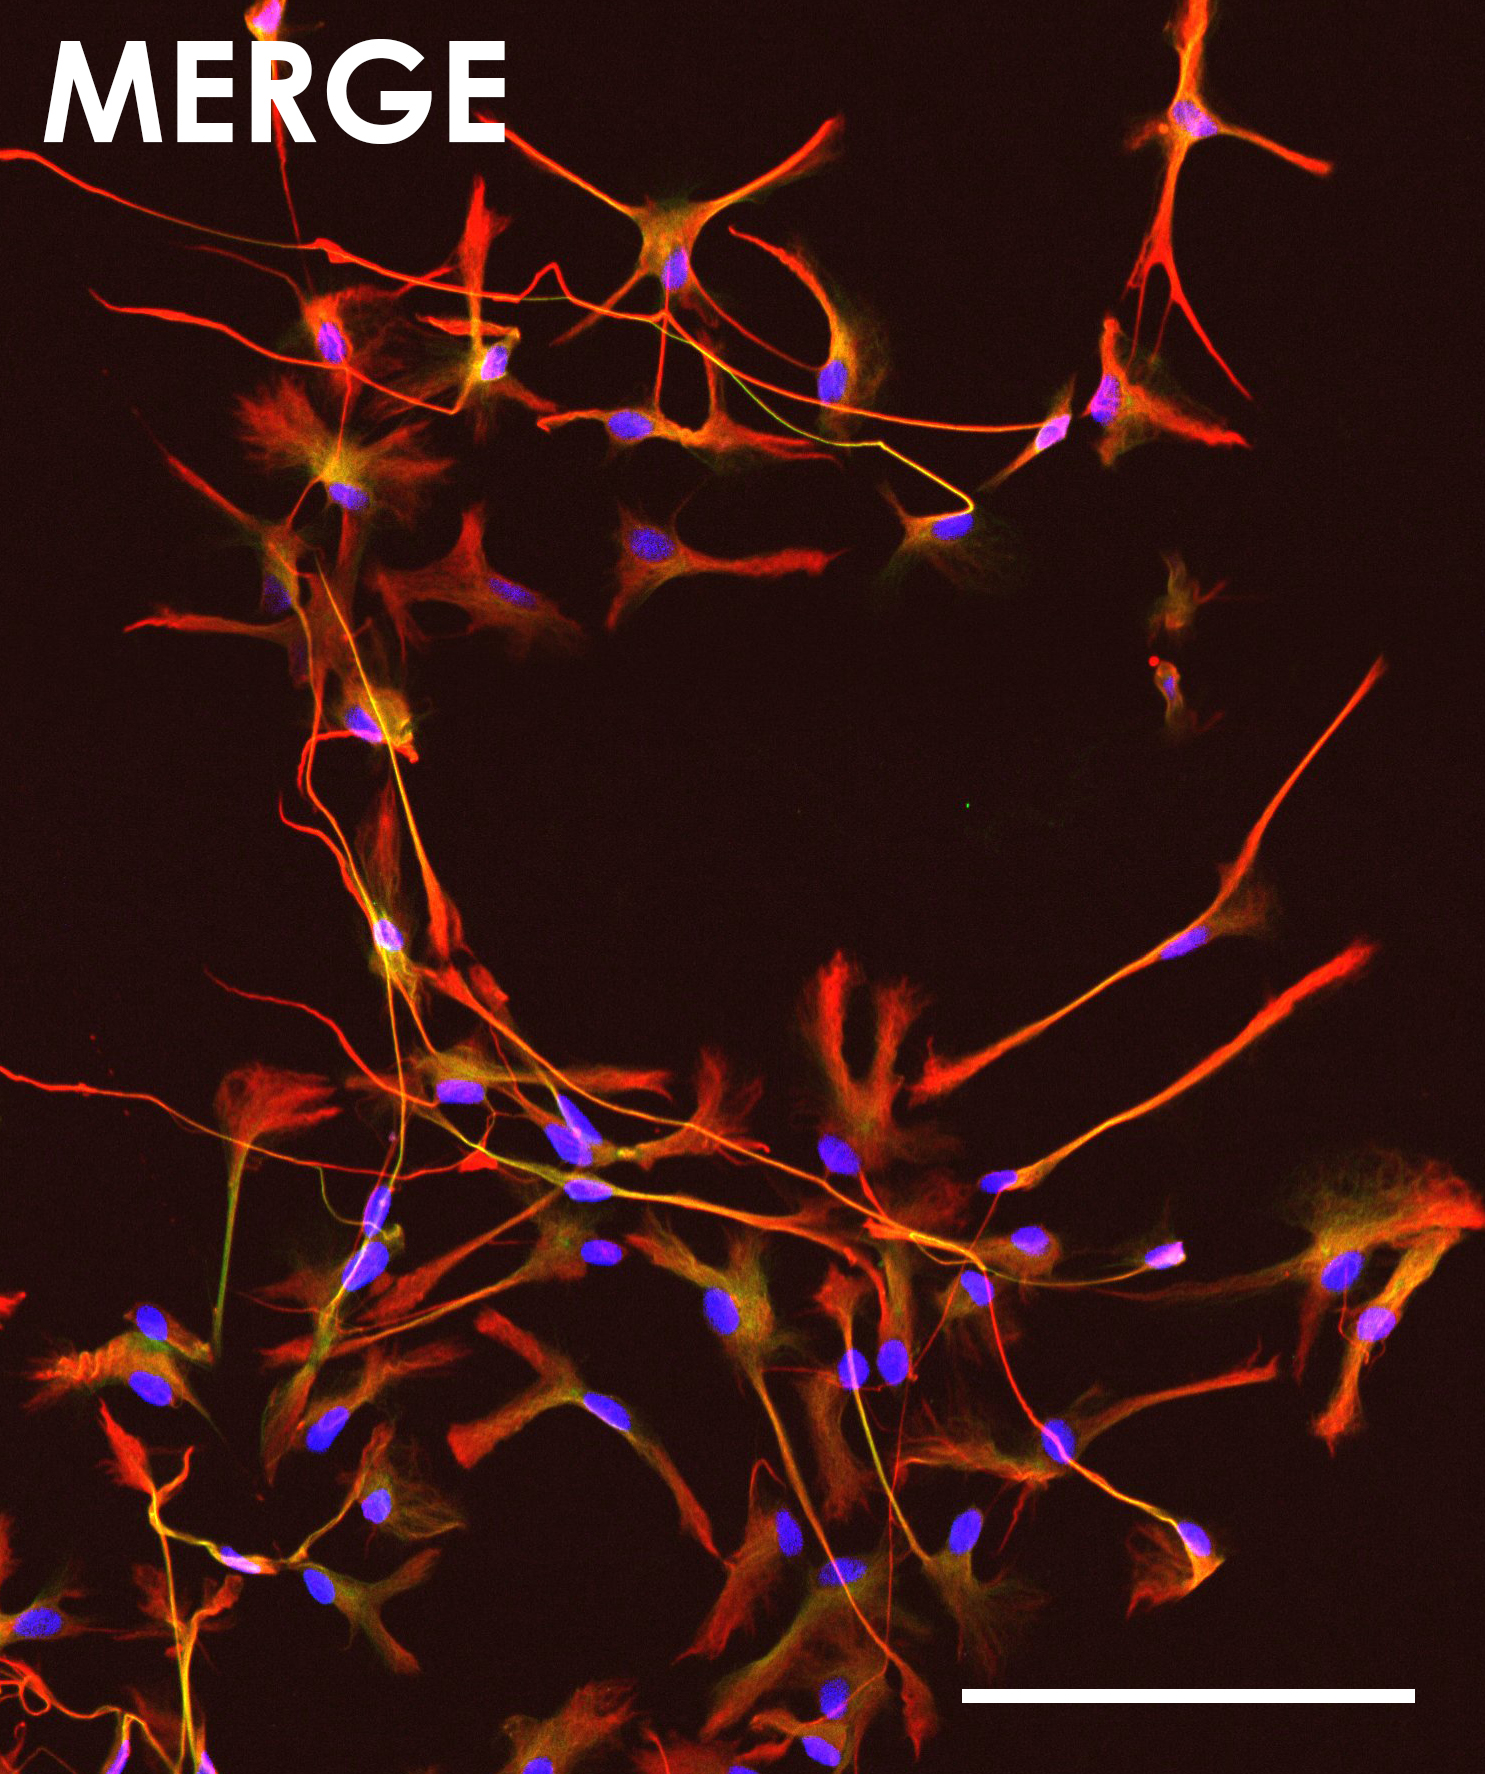
\includegraphics[width=0.196\textwidth]{figures/IF/charac(light)/d7-m}	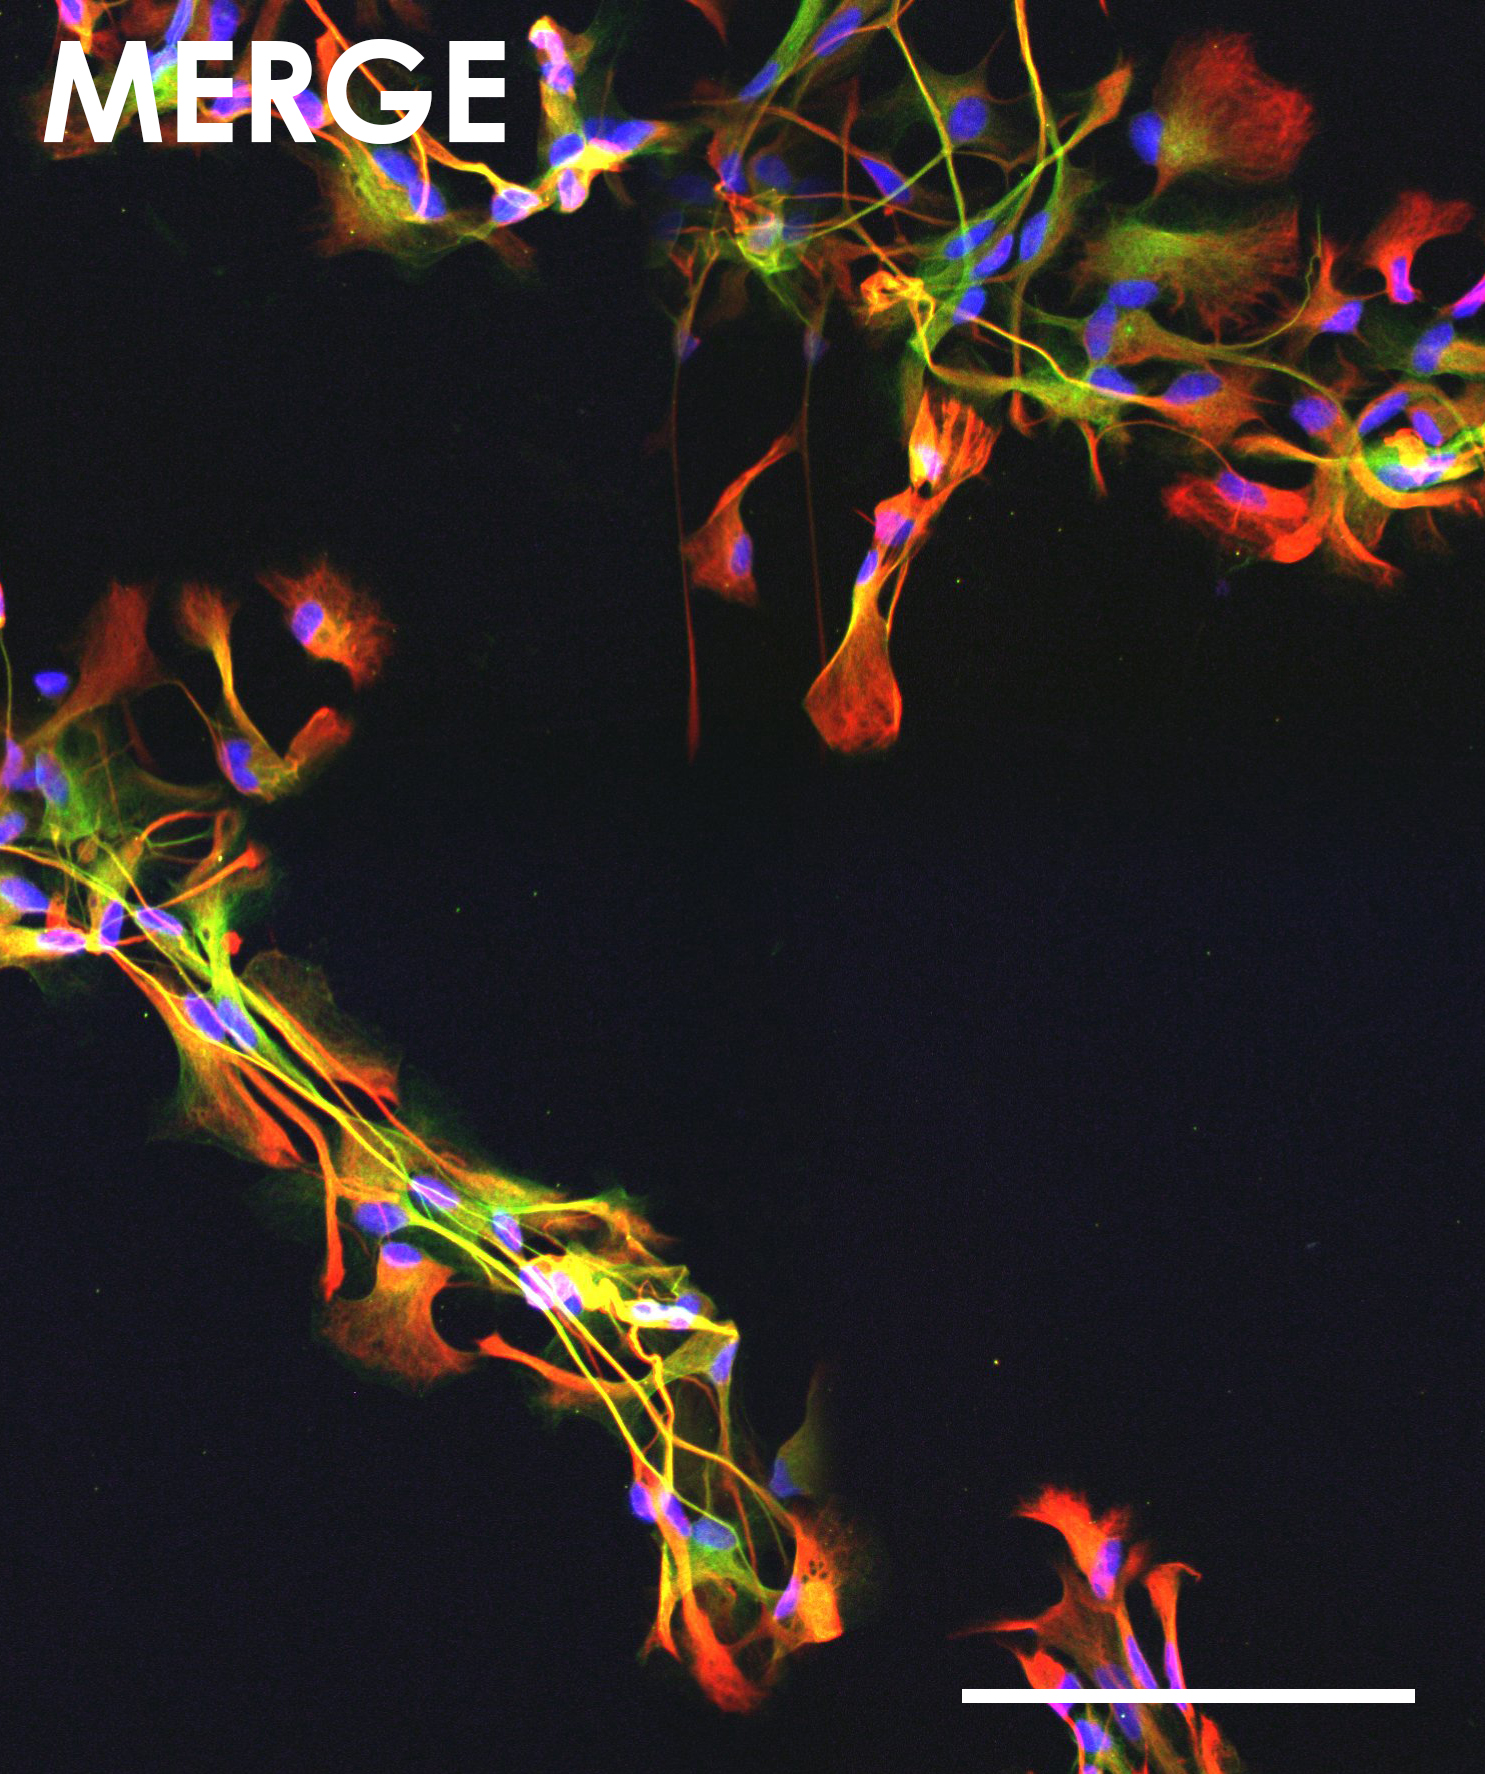
\includegraphics[width=0.196\textwidth]{figures/IF/charac(light)/d14-m}	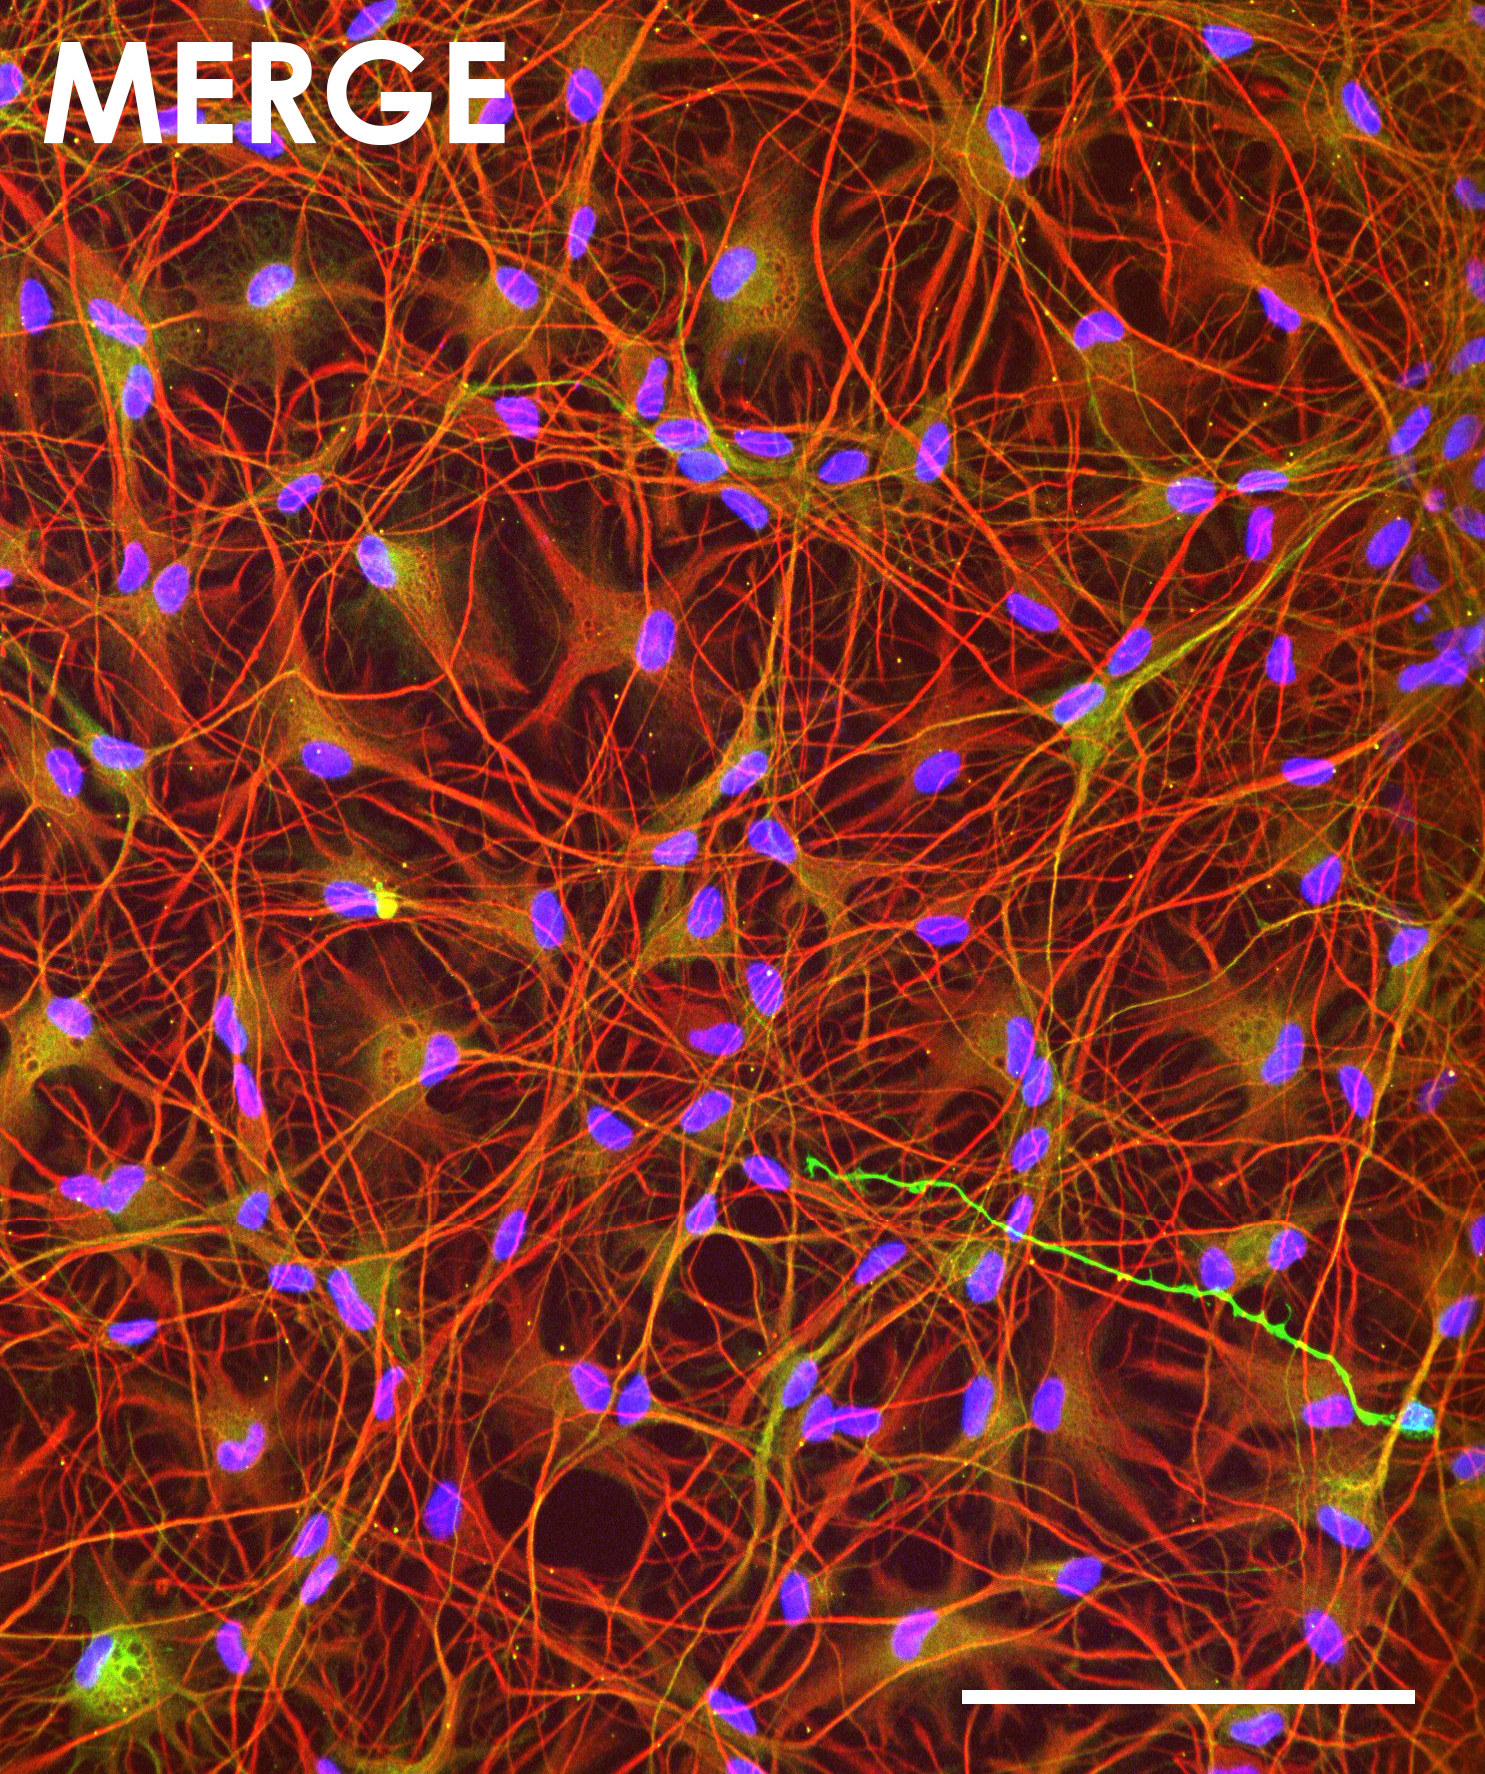
\includegraphics[width=0.196\textwidth]{figures/IF/charac(light)/d21-m}
	
	\caption{\textbf{Ren VM cells express a wide array of neural differentiation markers.} The differentiation capacity of ReNcell VM cells was assessed with immunofluorescence over 21 days with the indicated antibodies for n = 3 biological. Scale bars represent 500 um.}
	\label{diff-vm}
\end{figure}
\newpage

\begin{figure}[h]
	
	
	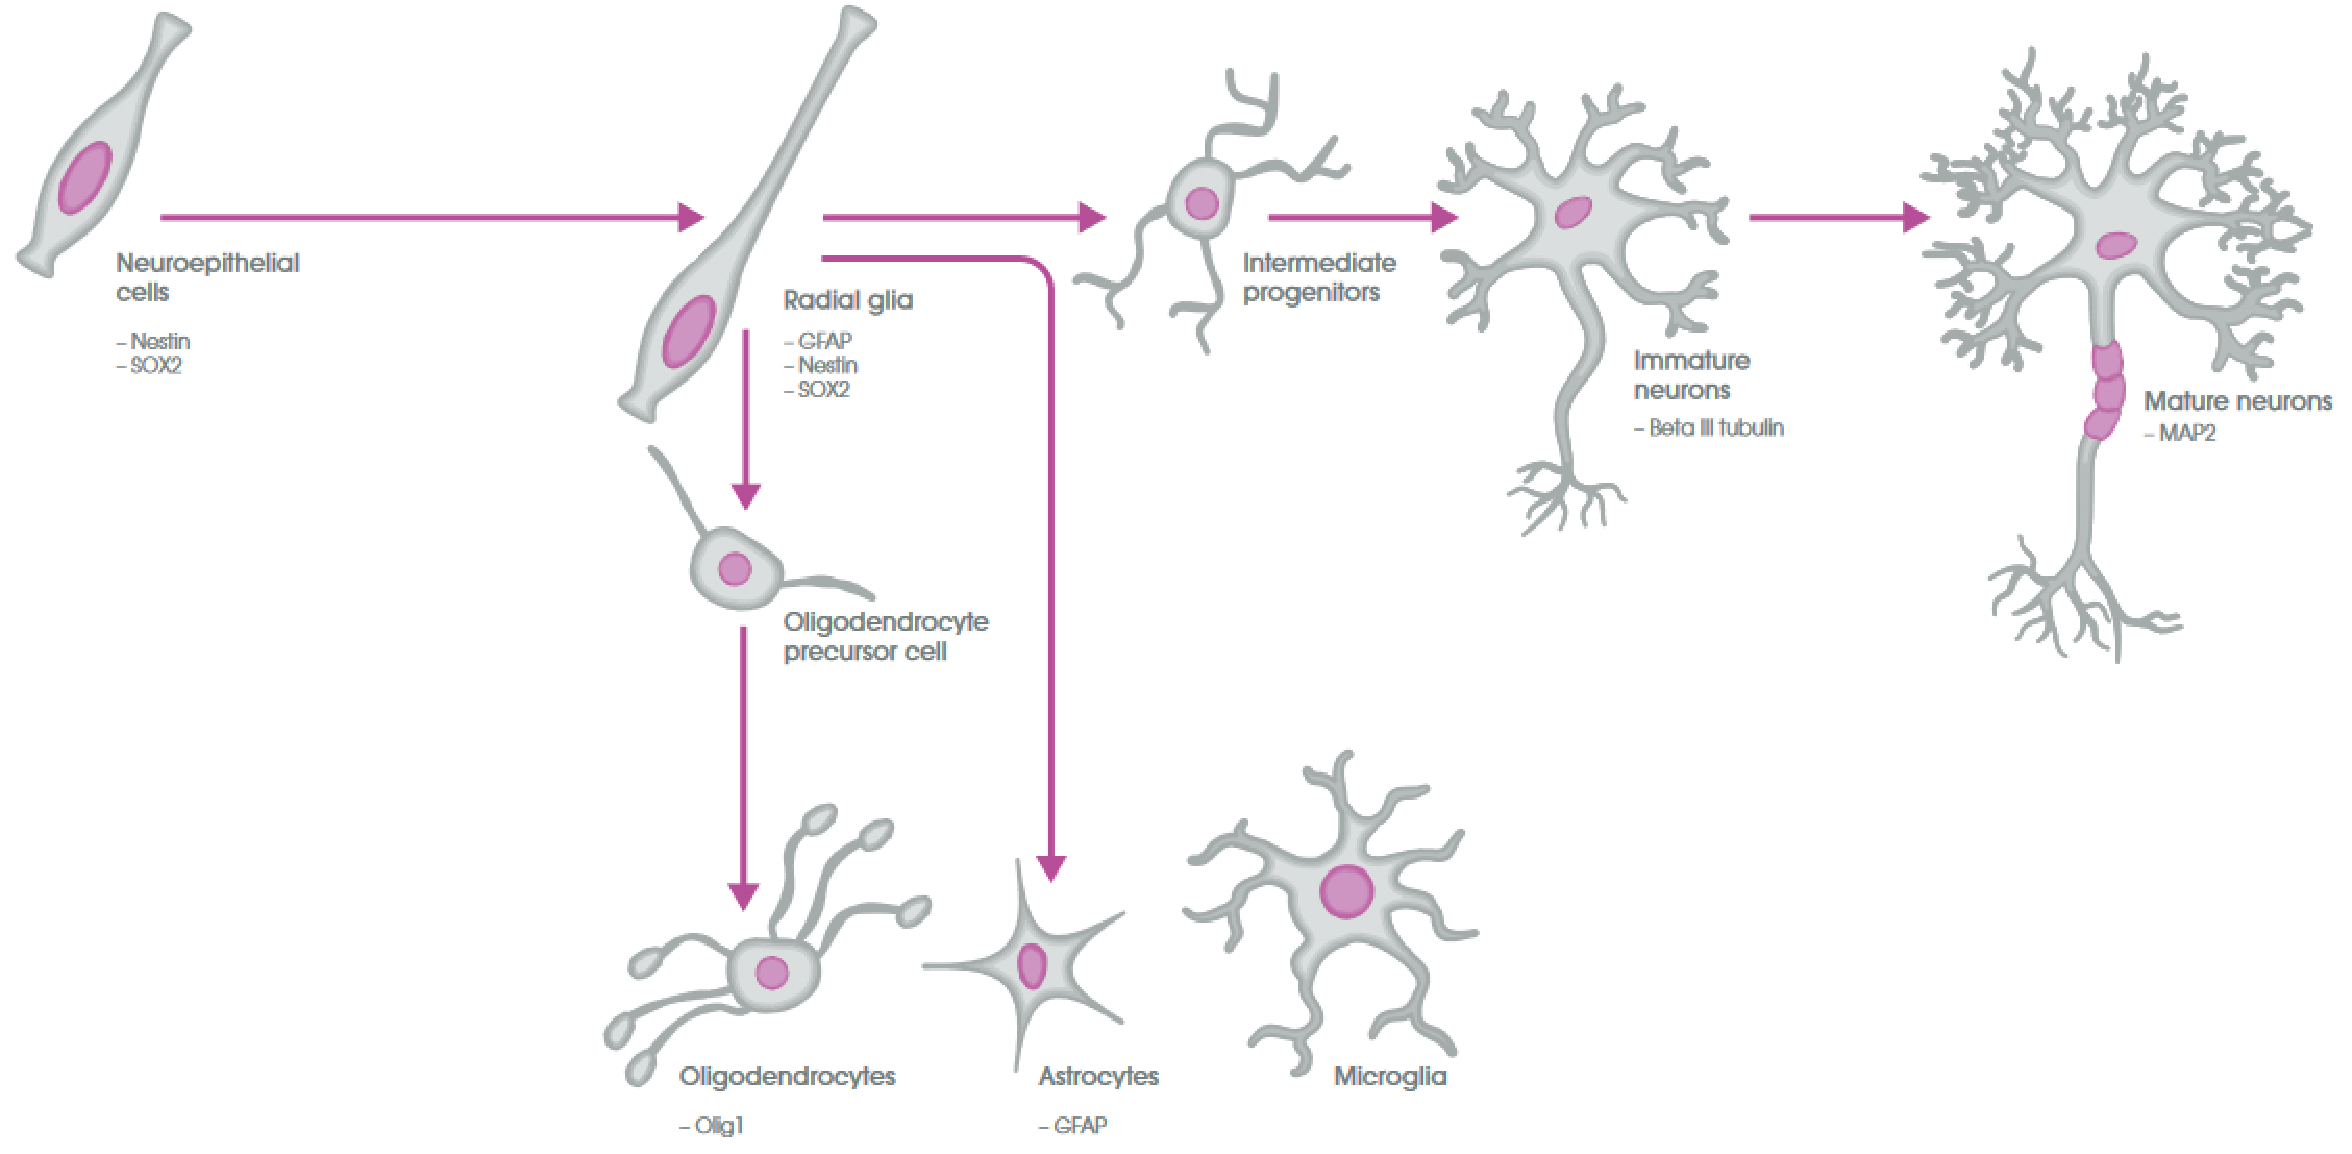
\includegraphics[width=\textwidth]{figures/neuron_marker}
	
	
	
\includegraphics[width=0.035\textwidth]{figures/IF/charac(light)/stain1}
	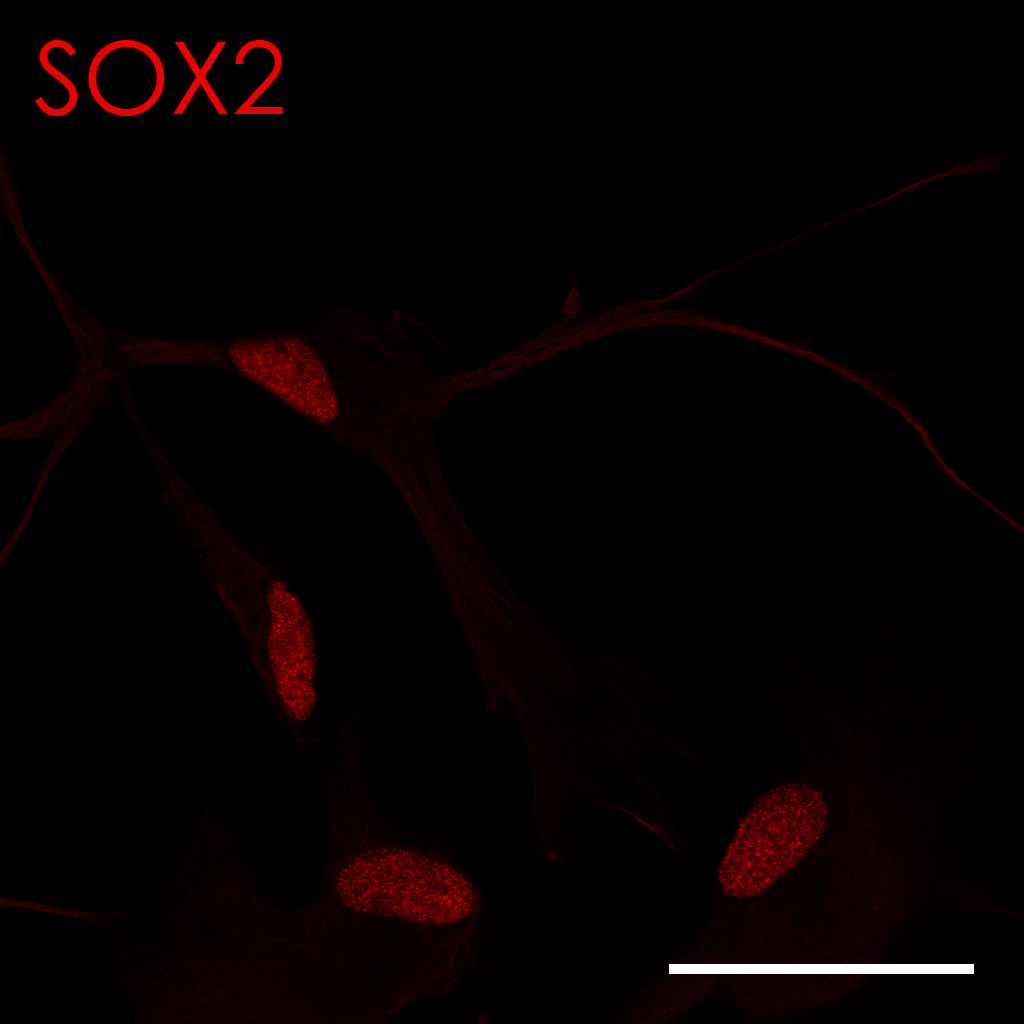
\includegraphics[width=0.235\textwidth]{figures/IF/charac(light)/SOX2(14)TUJ}
	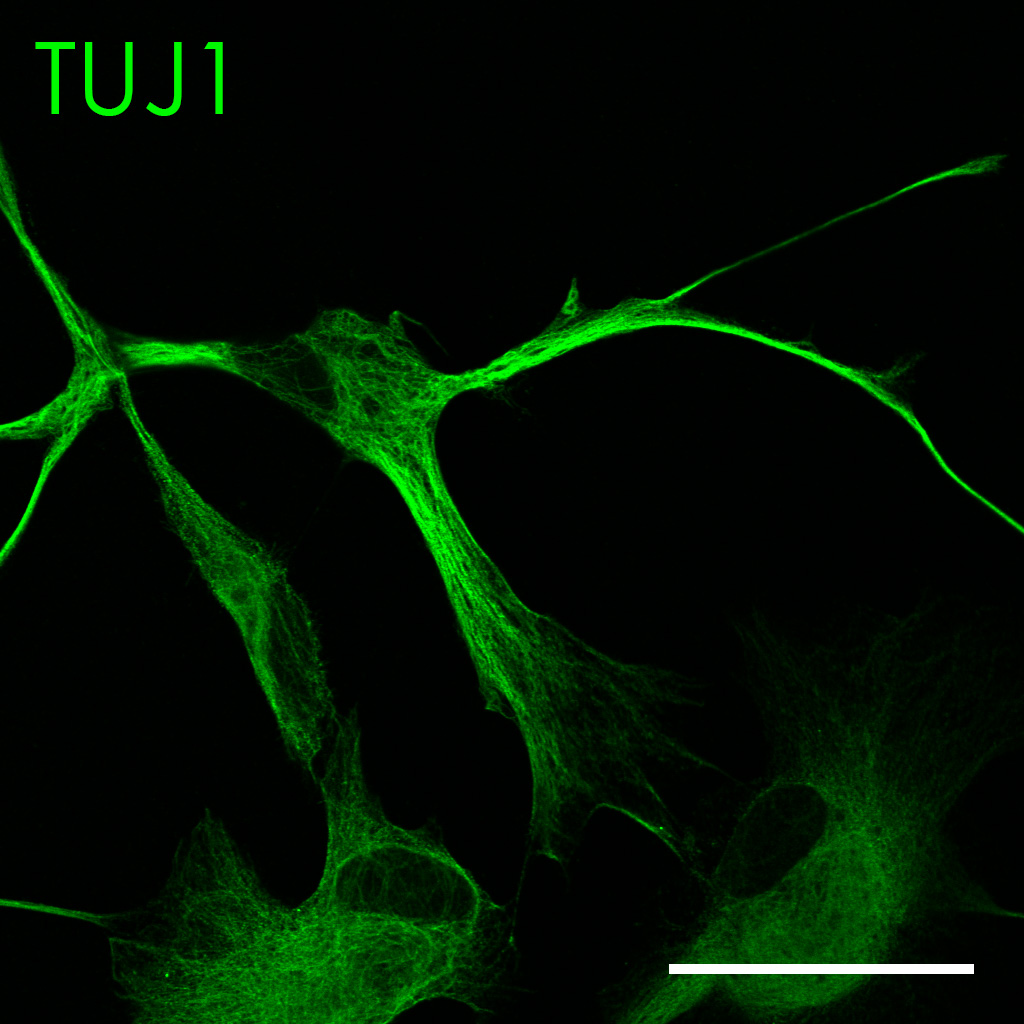
\includegraphics[width=0.235\textwidth]{figures/IF/charac(light)/TUJ1(14)TUJ}
	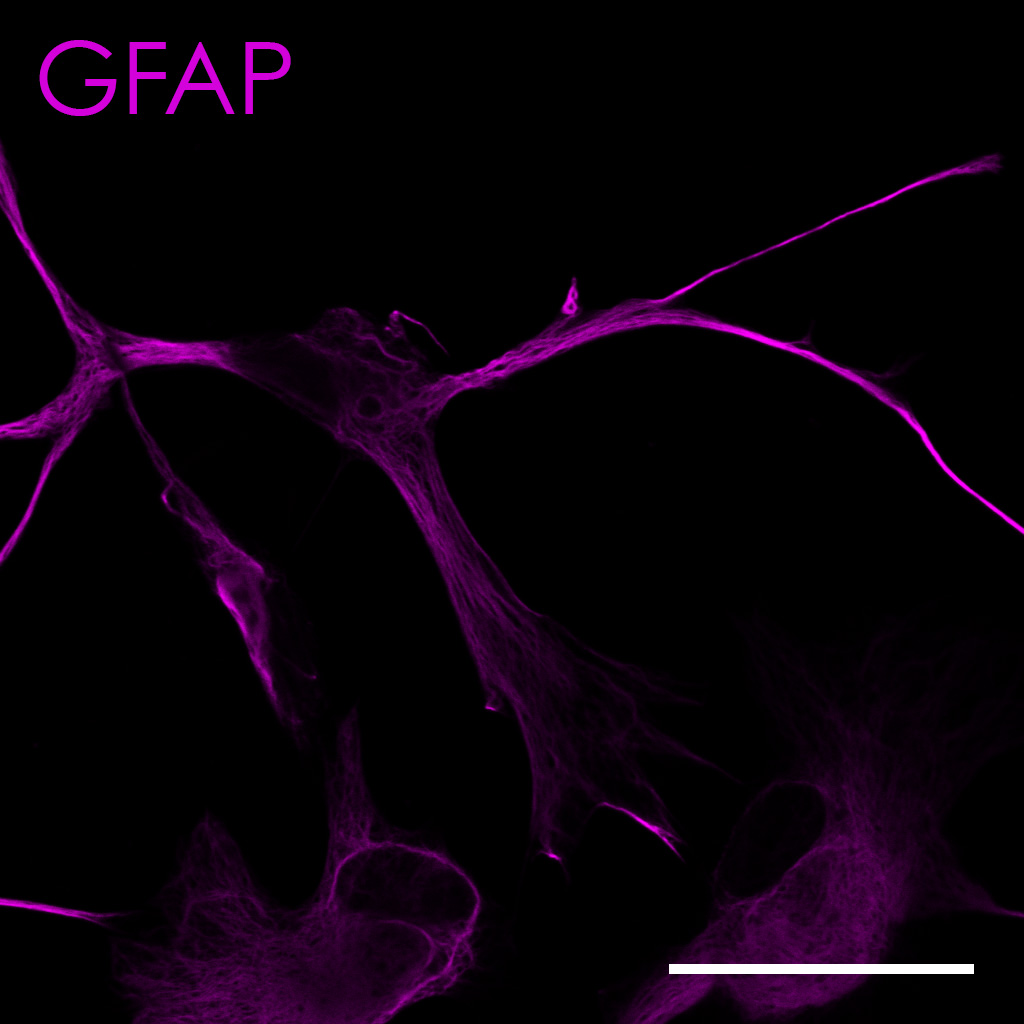
\includegraphics[width=0.235\textwidth]{figures/IF/charac(light)/GFAP(14)TUJ}
	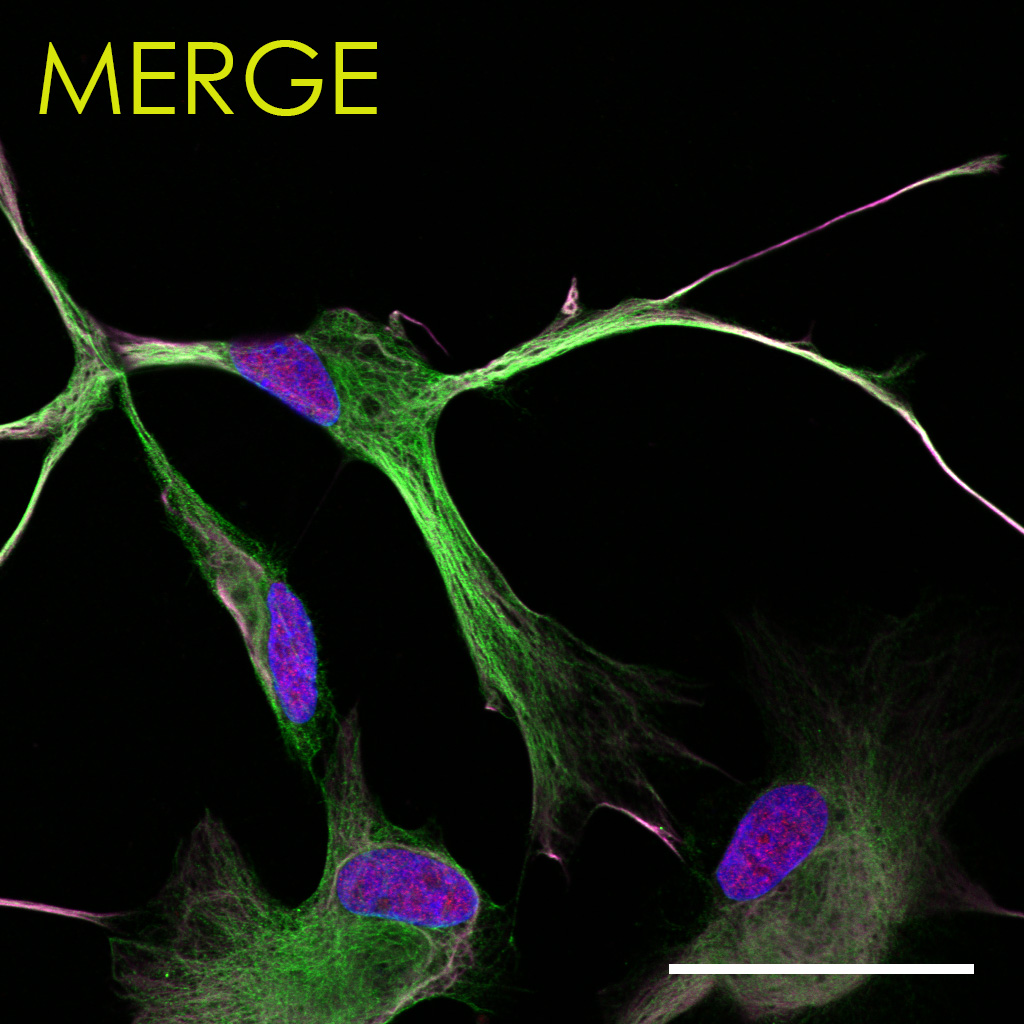
\includegraphics[width=0.235\textwidth]{figures/IF/charac(light)/MERGE(14)TUJ}
	
	
\includegraphics[width=0.035\textwidth]{figures/IF/charac(light)/stain2}
	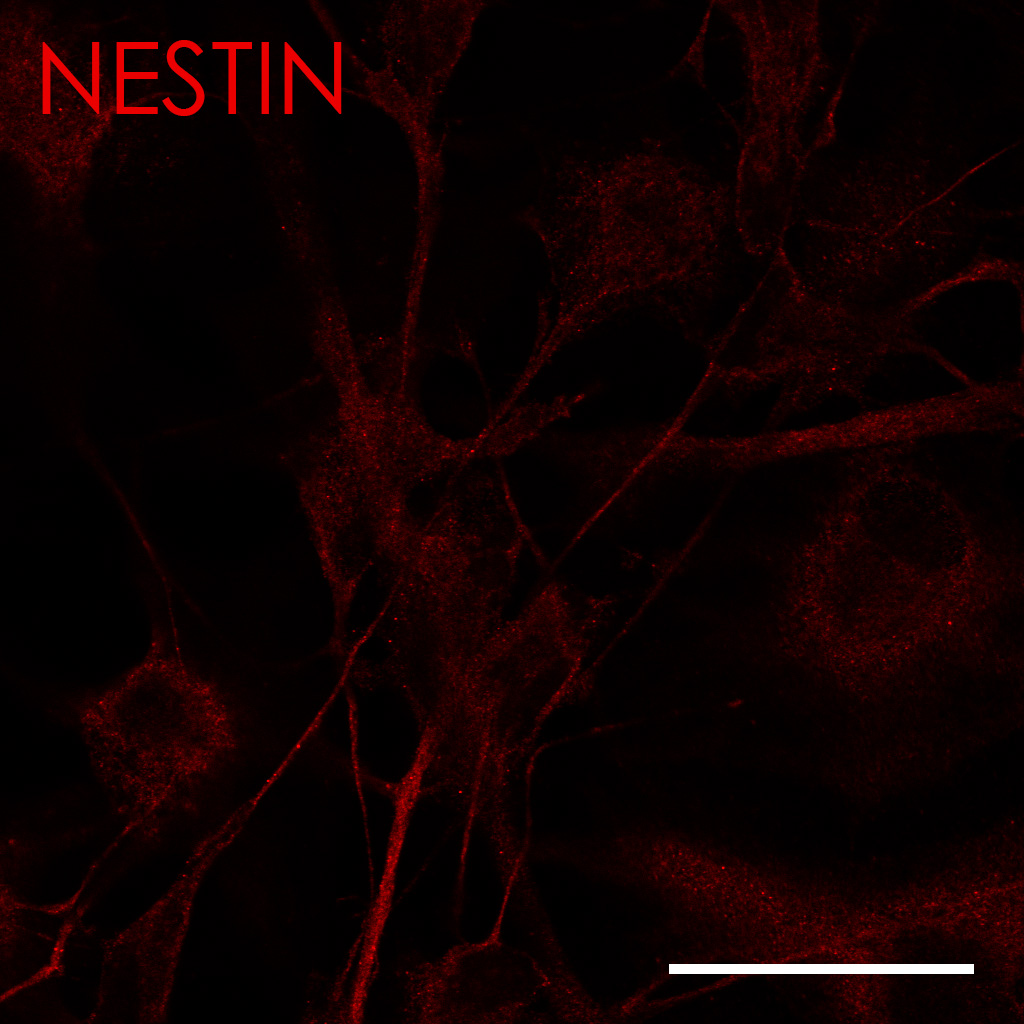
\includegraphics[width=0.235\textwidth]{figures/IF/charac(light)/NESTIN(14)GFAP}
	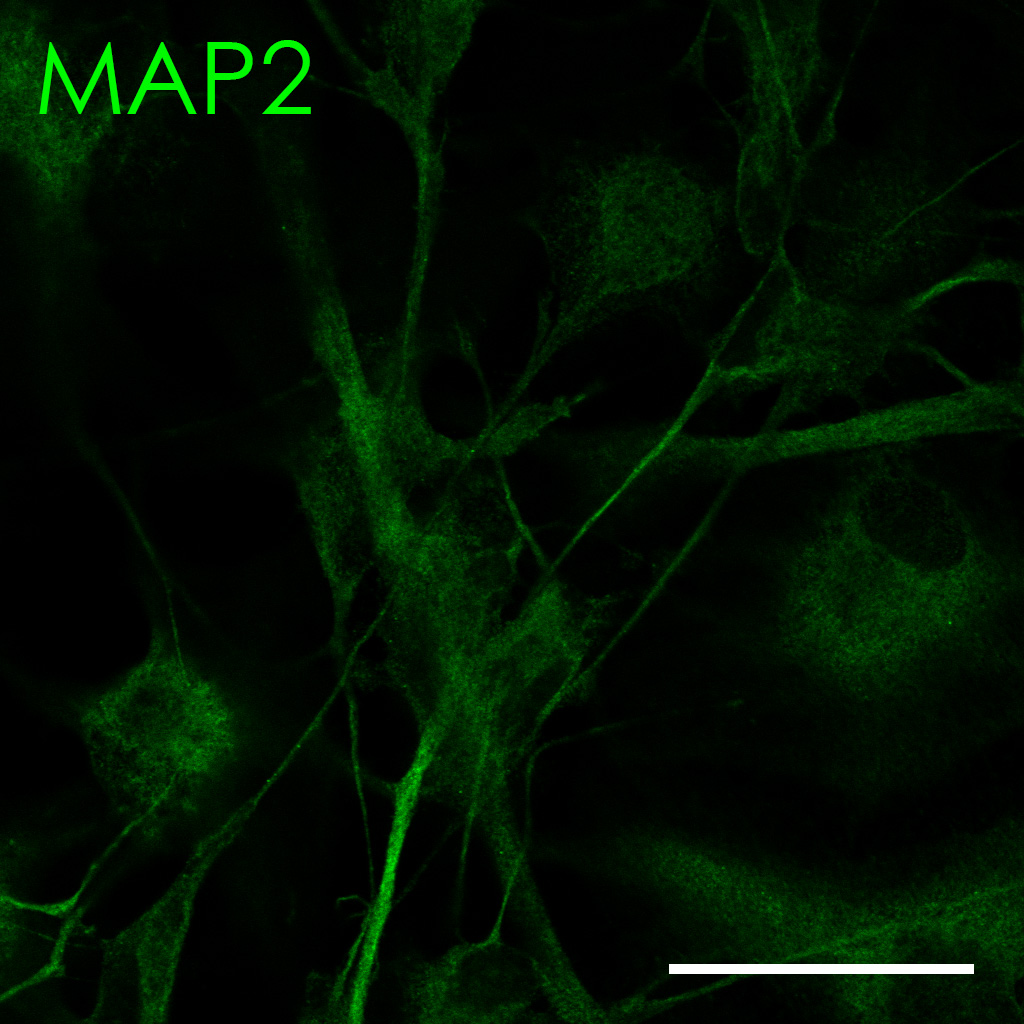
\includegraphics[width=0.235\textwidth]{figures/IF/charac(light)/MAP2(14)GFAP}
	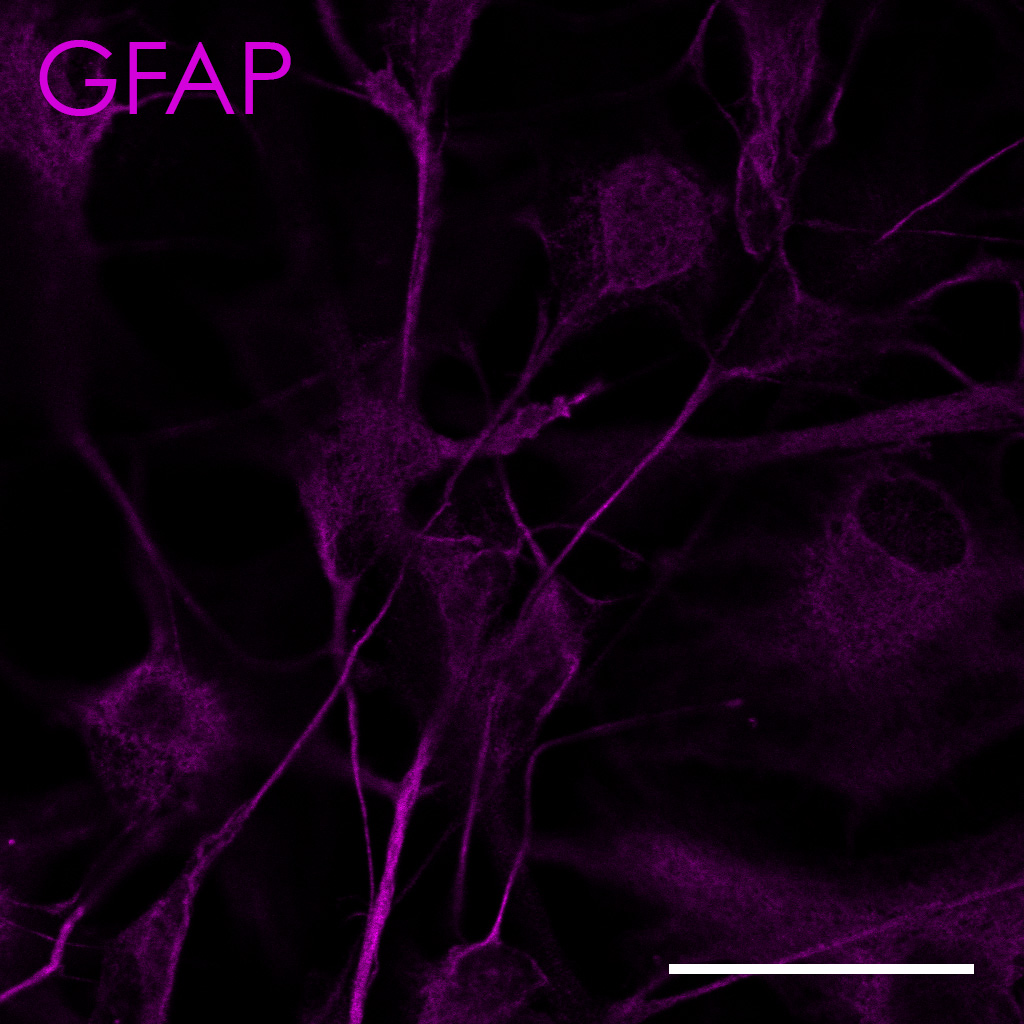
\includegraphics[width=0.235\textwidth]{figures/IF/charac(light)/GFAP(14)GFAP}
	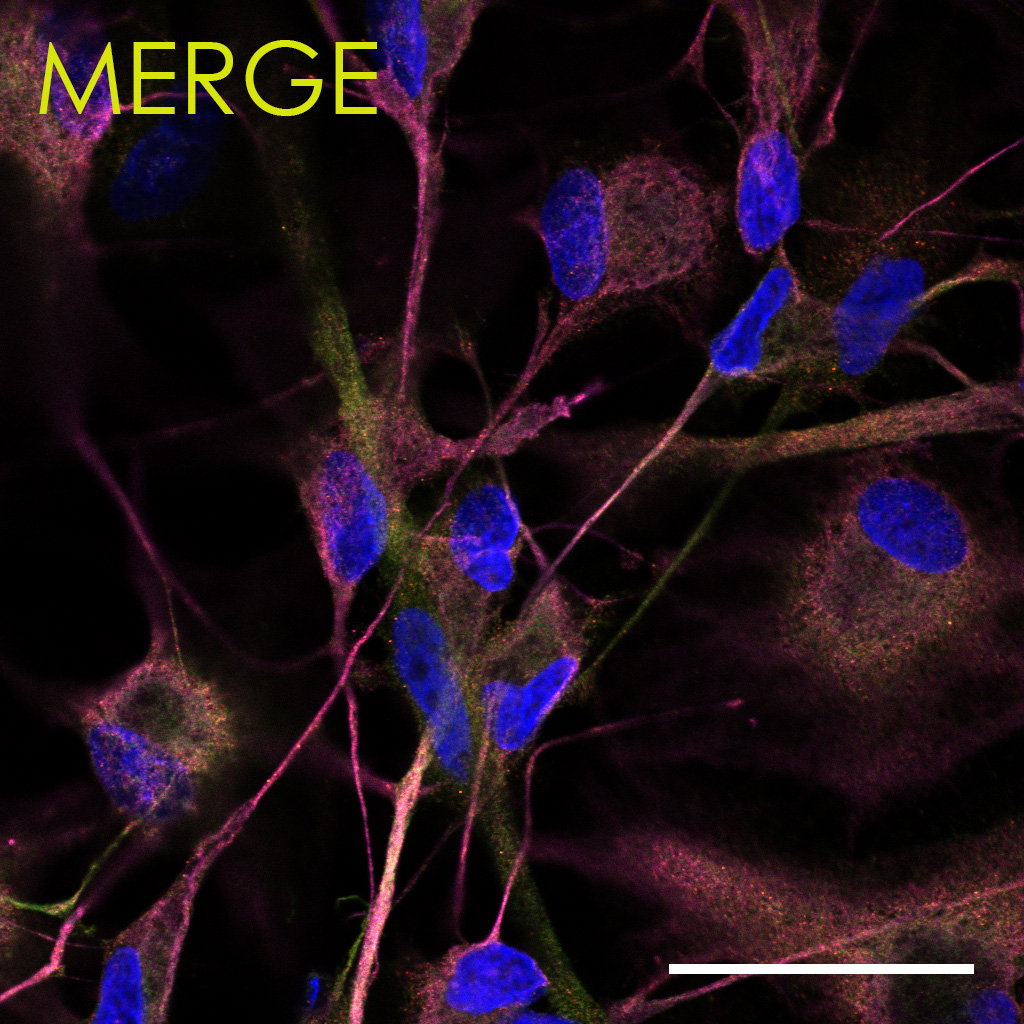
\includegraphics[width=0.235\textwidth]{figures/IF/charac(light)/MERGE(14)GFAP}
	
	
\includegraphics[width=0.035\textwidth]{figures/IF/charac(light)/stain3}
	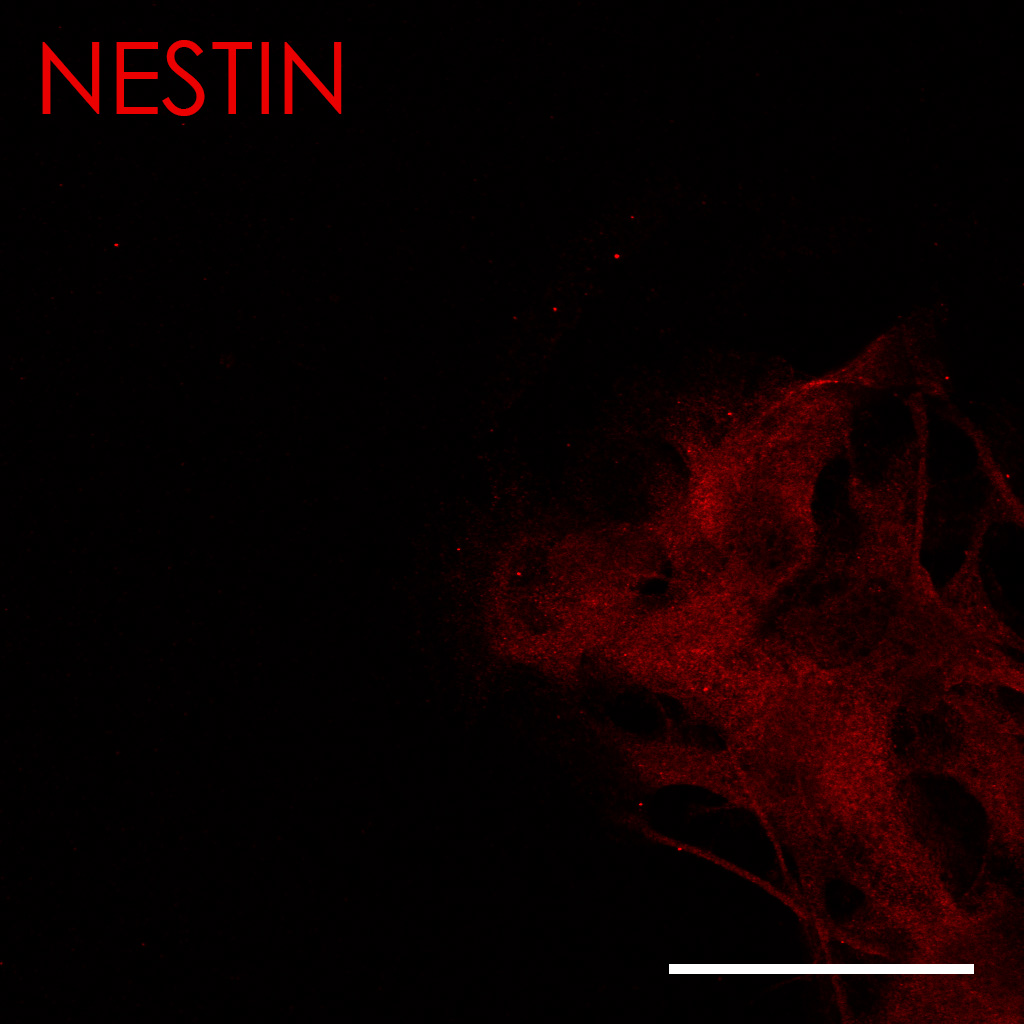
\includegraphics[width=0.235\textwidth]{figures/IF/charac(light)/NESTIN(14)OLI}
	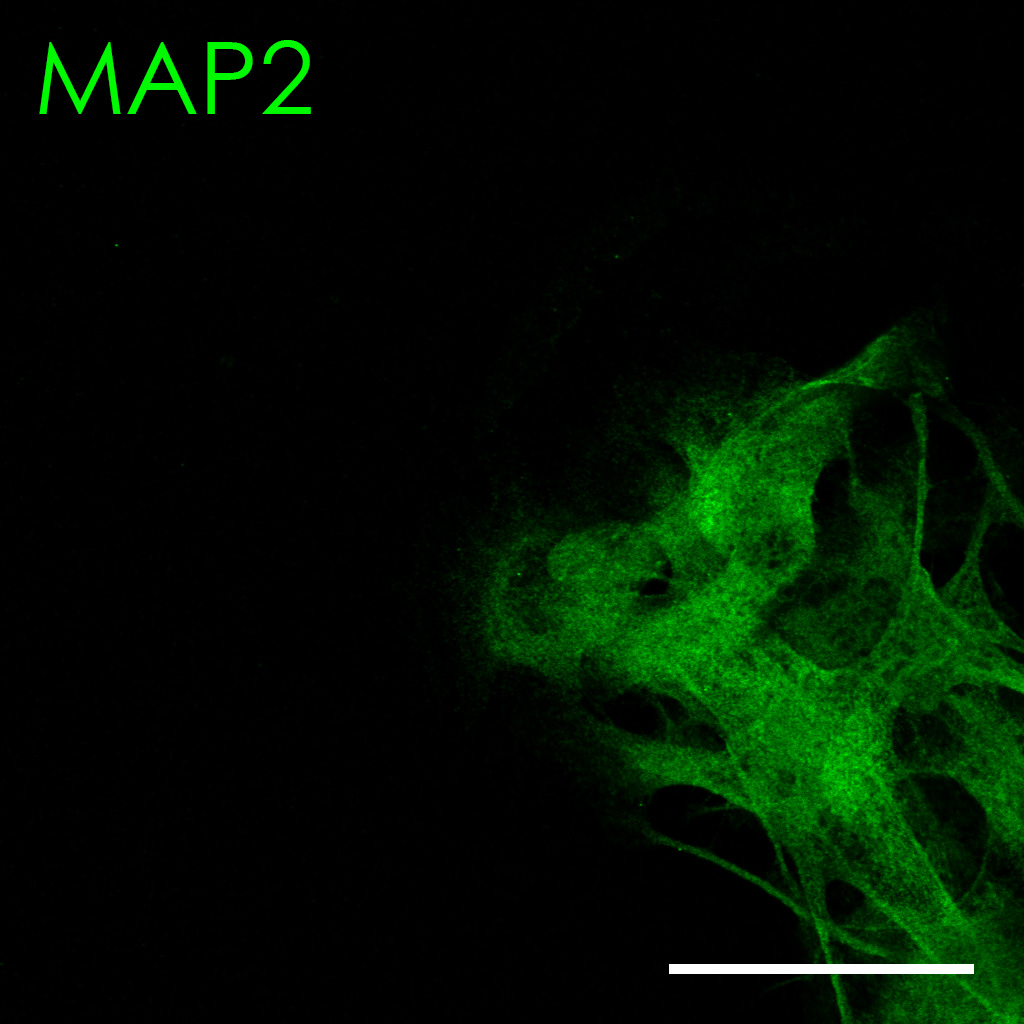
\includegraphics[width=0.235\textwidth]{figures/IF/charac(light)/MAP2(14)OLI}
	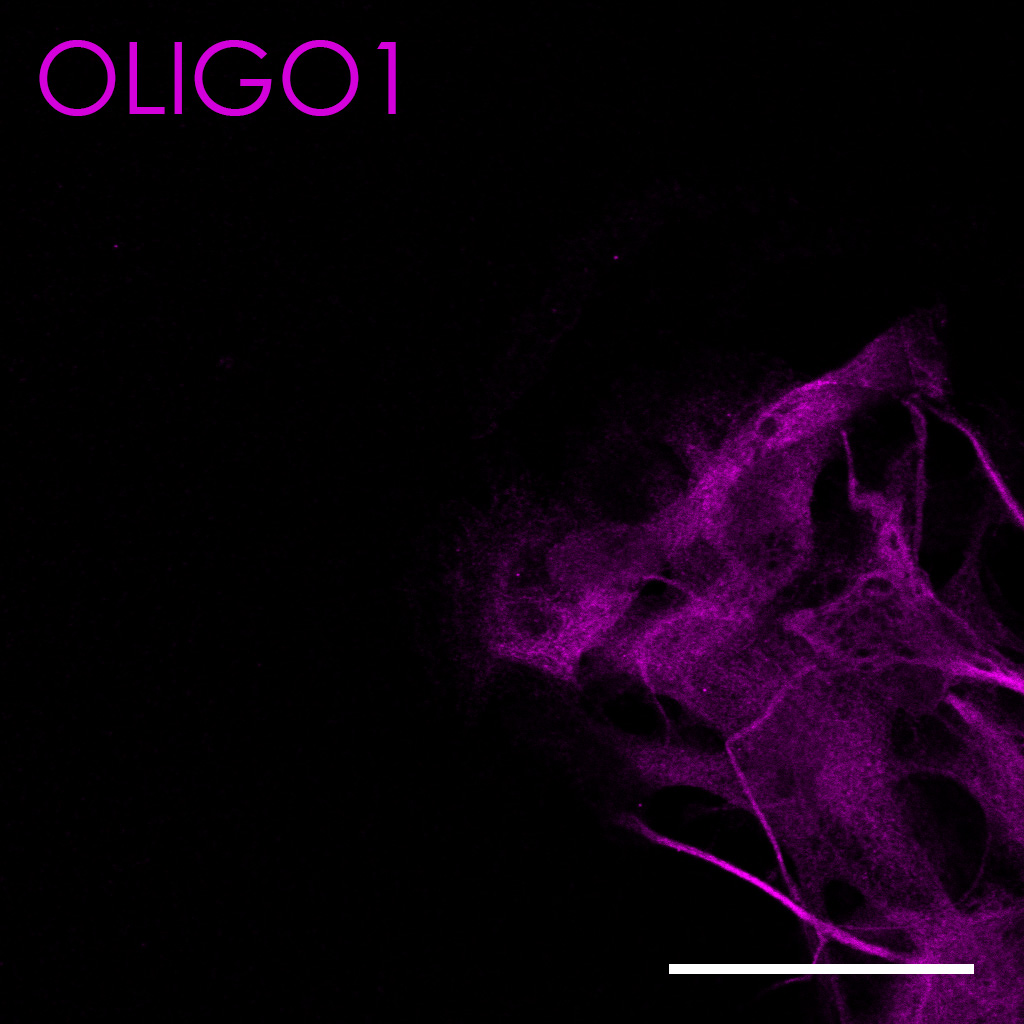
\includegraphics[width=0.235\textwidth]{figures/IF/charac(light)/OLIGO1(14)OLI}
	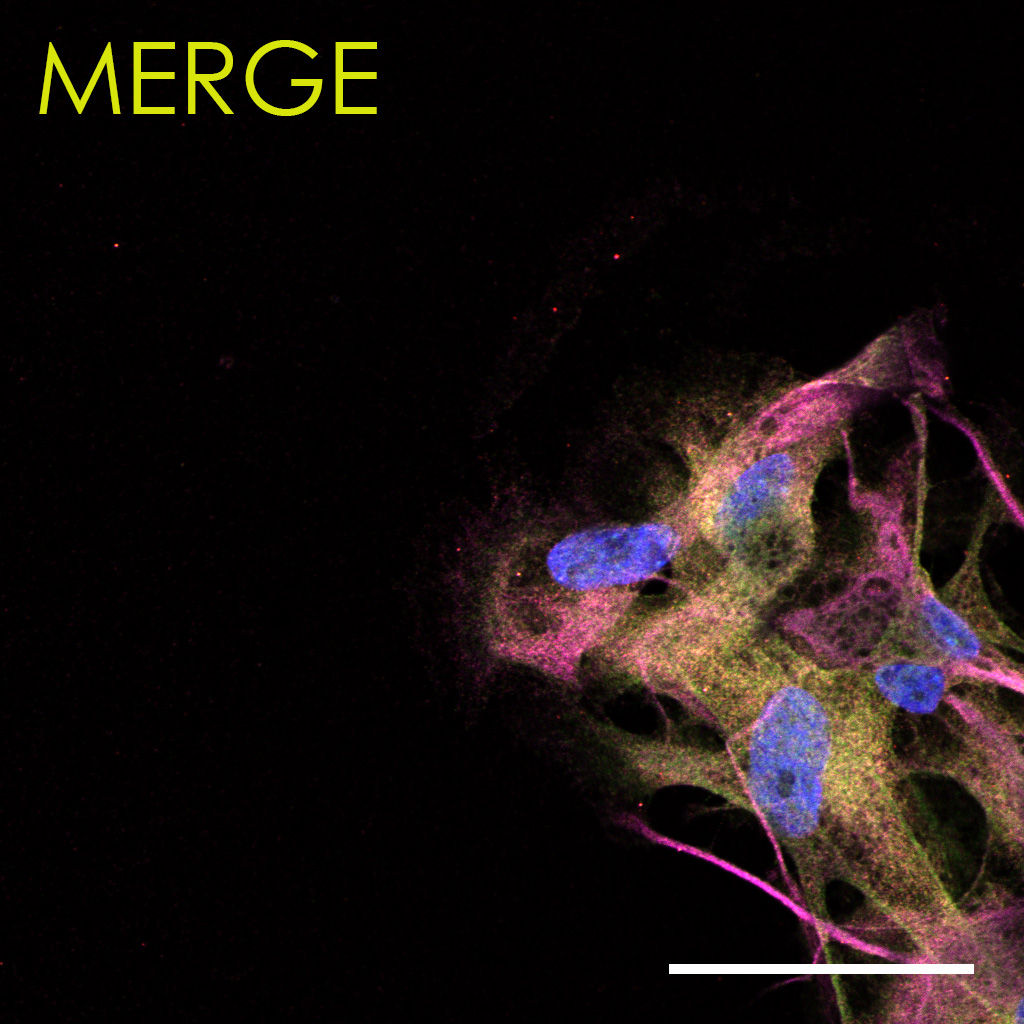
\includegraphics[width=0.235\textwidth]{figures/IF/charac(light)/MERGE(14)OLI}
	
	\caption{\textbf{Optimisation of IF stain on D-14 differentiated cells.} (A) Cells were cultured in growth-factor free medium for 7 days. (B) In parallel, cells were culture for 4 days in differentiation medium, radiated with 2 Gy and stained 3 days later. Scale bars represent 40um.	
		These cells are basically positive for all the markers (at least at day 14) which shows they go from progenitor cells to more differentiated progenitor cells but do not reach full maturation (at least not at day 14). 
		(A) adapated from Abcam's neural marker website. 
		TUJ1: marker for mature neurons.
		SOX2: marker for stem cells.
		In blue, counterstained with DAPI.
		% MUST ADD THE LABEL FOR SIZE
	}
	\label{stain-opti}
\end{figure}
\newpage


\subsubsection{The SY5Y cell line}
The SY5Y cells are equally capable of differentiation which was assessed in the same manner as before. Cells were harvested on days 0, 3, 7, 14 and 21 and stained with the same markers as Figure \ref{diff-vm}. However, this neuroblastoma cell line only generates (?) neurons, justifying why GFAP and SOX2 were used as negative controls. Indeed, the cells did not express either of these markers (not shown here), but were positive for Tuj1. Once again, no dramatic increase or decrease of Tuj1 expression was witnessed over 21 days in retinoic-acid supplemented medium. Similarly to the VM cells, the morphology of the SY5Y cells provided a reliable measure of the differentiation stage, where the cells elongated drastically to form neurites. 


%\subsection{Bioreactor development}




\begin{figure}[h]
	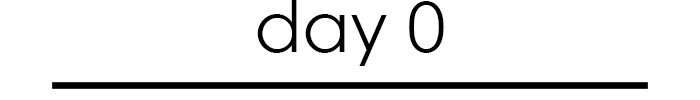
\includegraphics[width=0.196\textwidth]{figures/IF/charac(light)/d0}
	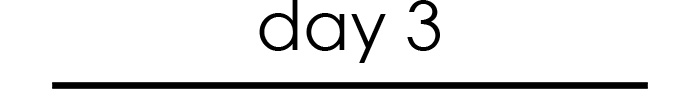
\includegraphics[width=0.196\textwidth]{figures/IF/charac(light)/d3}
	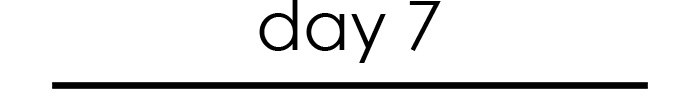
\includegraphics[width=0.196\textwidth]{figures/IF/charac(light)/d7}
	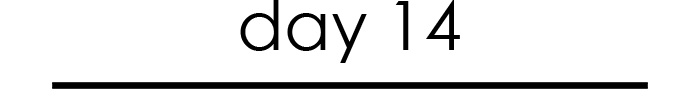
\includegraphics[width=0.196\textwidth]{figures/IF/charac(light)/d14}
	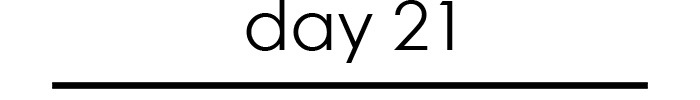
\includegraphics[width=0.196\textwidth]{figures/IF/charac(light)/d21}
	
	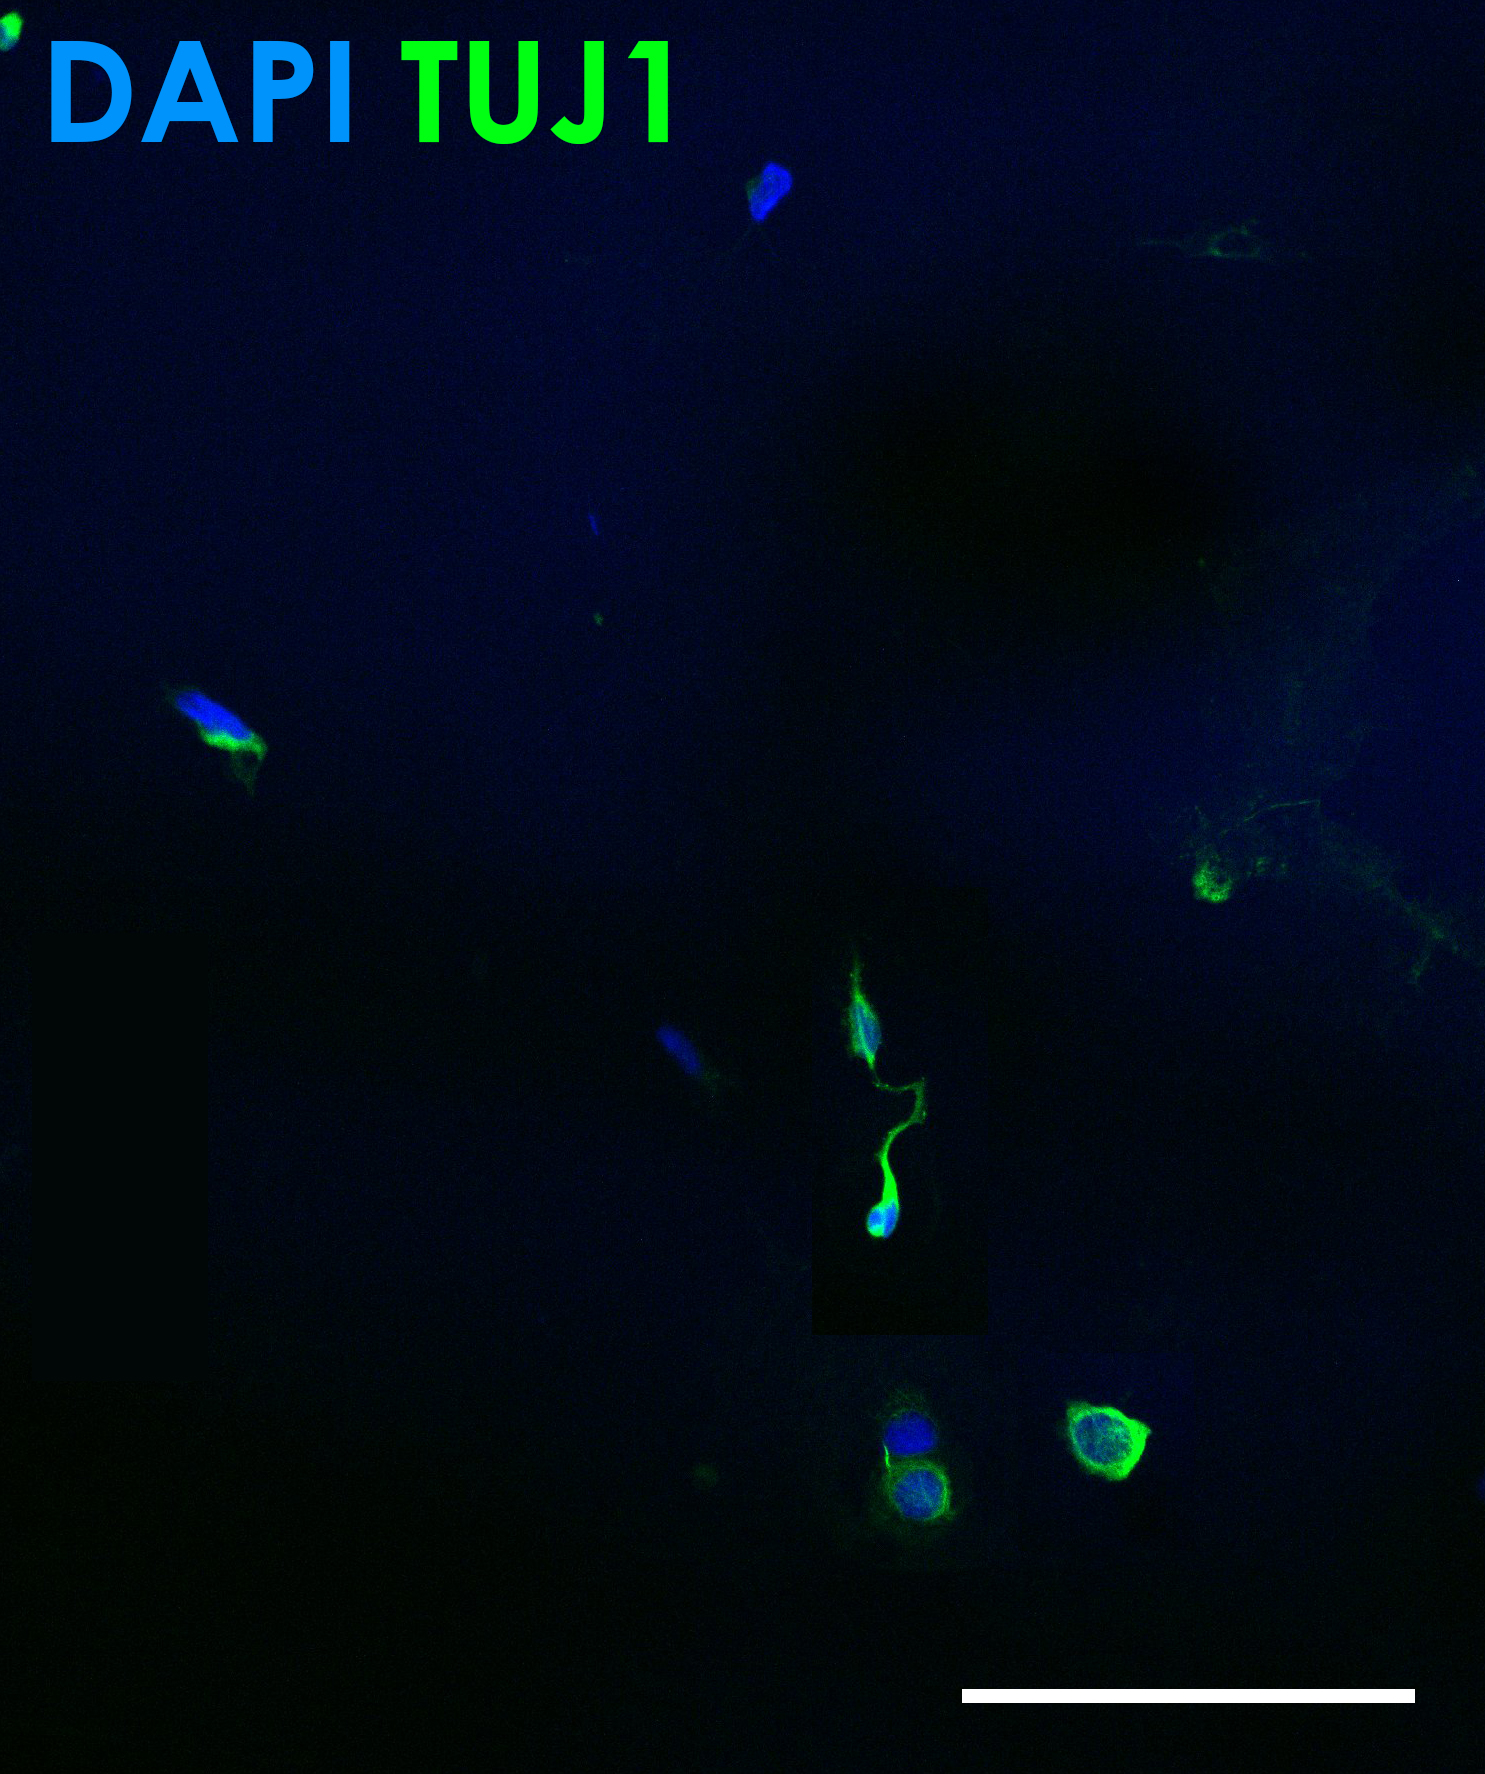
\includegraphics[width=0.196\textwidth]{figures/IF/SY5Y/d0-t}
	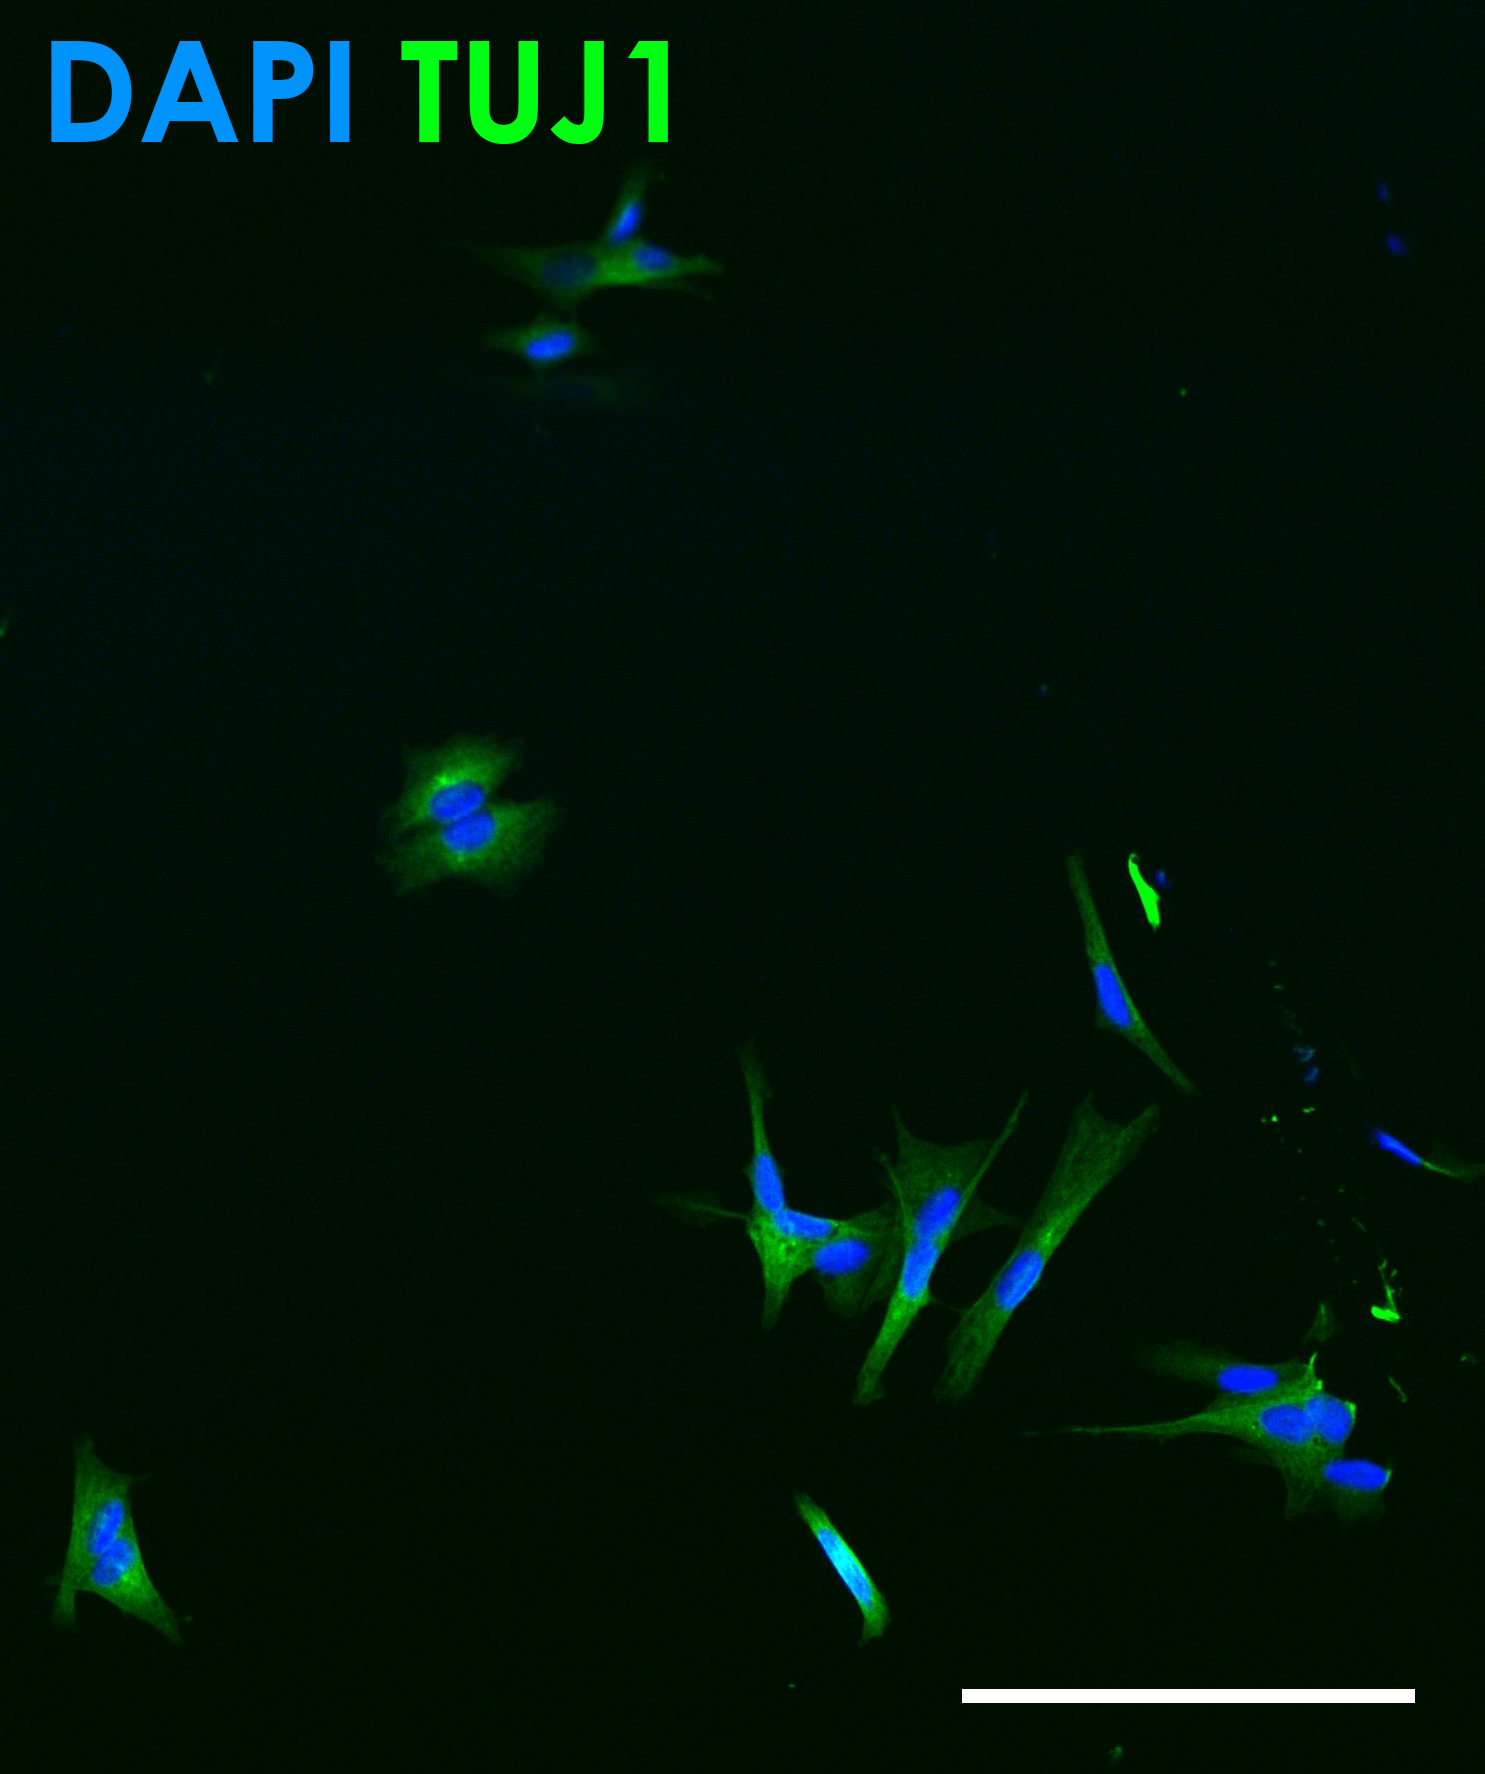
\includegraphics[width=0.196\textwidth]{figures/IF/SY5Y/d3-t}
	\includegraphics[width=0.196\textwidth]{figures/IF/SY5Y/d7-t.jpg}
	\includegraphics[width=0.196\textwidth]{figures/IF/SY5Y/d14-t}
	\includegraphics[width=0.196\textwidth]{figures/IF/SY5Y/d21-t}
	\caption{\textbf{SY5Y cells express neuronal differentiation markers.} The differentiation capacity of ReNcell VM cells was assessed with immunofluorescence over 21 days with the indicated antibodies for n = 3 biological repeats. Scale bars represent 500 um.}
	\label{diff-sy5y}
\end{figure}


\subsection{Drug inhibition}

\subsubsection{DYRK1A inhibition and transient knockout}
To apprehend the functional implications of DYRK1A in the differentiation pathway of neural cells, the VM cells were transfected with an siRNA on the kinase. However, the neural stem cells are especially fragile and difficult to transfect so three protocols were tested:  4d Nucleofector, Lipofectamine 2000 and Lipofectamine RNAiMAX. 
In both lipofections, a GFP plasmid was inserted to allow assessment of transfected cells by fluoroscope microscopy.
As shown in Figure \ref{transfection}, the electroporation yeilded significantly more GFP positive cells (p value < X, 4d Nucleofector vs Lipofectamine 2000, p < 4d Nucleofector vs Lipofectamine RNAiMAX)(?). 

%These experiments were drawn before the SY5Y cells were acquired and not repeated on these cells as the focus of the project shifted from DYRK1A and narrowed on radiation.


The SY5Y cells were transfected solely with lipofections without GFP (according to Thermo Fisher's protocols) which is a cheaper alternative to electroporation which is quite efficient on robust cell lines such as cancer cells. 

To verify the specificity of the siRNA and the efficiency of the transfection, the cells were harvested 48 hours after transfection and DYRK1A expression was evaluated by Western Blot. As Figure \ref{transfection} shows, the transfection on the VM cells did not yield a significant decrease of the kinase. Due to limited time, the focus of the project shifted away from transient knockout of DYRK1A.

\begin{figure}[h]
	\includegraphics[width=0.05\textwidth]{figures/a}
	
	
	\includegraphics[width=0.33\textwidth]{figures/electro/Nucleo.jpg}
	\includegraphics[width=0.33\textwidth]{figures/electro/Lipo2000.jpg}
	\includegraphics[width=0.33\textwidth]{figures/electro/LipoMAX.jpg}
	
	
	\includegraphics[width=0.33\textwidth]{figures/electro/ctrl-elec.jpg}
	\includegraphics[width=0.33\textwidth]{figures/electro/BF2000(D1).jpg}
	\includegraphics[width=0.33\textwidth]{figures/electro/BFMAX(D3).jpg}
	
	\includegraphics[width=0.33\textwidth]{figures/electro/ctrl-elec-g.jpg}
	\includegraphics[width=0.33\textwidth]{figures/electro/G2000(D1).jpg}
	\includegraphics[width=0.33\textwidth]{figures/electro/GMAX(D3).jpg}
	
	\includegraphics[width=0.33\textwidth]{figures/electro/ctrl-elec-m.jpg}
	\includegraphics[width=0.33\textwidth]{figures/electro/Compo2000.jpg}
	\includegraphics[width=0.33\textwidth]{figures/electro/CompoMAX.jpg}
	
	
	
	\includegraphics[width=0.05\textwidth]{figures/b}
	
	
	\begin{center}
		\includegraphics[width=0.3\textwidth]{figures/transfection.jpg}		
	\end{center}
	
	
	
	\includegraphics[width=0.05\textwidth]{figures/c}
	
	
	\begin{center}
		\includegraphics[width=0.8\textwidth]{figures/wb-sirna.jpg}	
	\end{center}
	
	\caption{\textbf{Transfection of Ren VM cells with DYRK1A siRNA.} Cells were transfected with DYRK1A siRNA by using the LONZA 4d Nucleofector protocol on primary cell lines. This was done with three different siRNA concentrations (100, 200 and 300 nM), with a mock (no DNA was added) and a negative control (luciferase). For n = 4, transfection efficiency is 33.75\% Unfortunately, the cells died before any quantifiable data was acquired - to be repeated. Might want to try with Lipofectamine considering electroporation is pricey (the cuvettes).
		Maybe put the WB in the annexe?
		Scale bar = 200 um.}
	\label{transfection}
\end{figure}


Instead, three well-known DYRK1A inhibitors were investigated. The initial step to pinpoint the effect of these drugs on both VM and SY5Y cells was to run a cytoxicity assay. This was carried out with a colorimetric AlamarBlue assay on both cell lines. The VM responded a lot quicker than the SY5Y, and a lot more heterogeneously. From preliminary data (not shown here), the third drug of choice, INDY, pointed to interesting results, which justifies why the following three repeats of this experiment used a range of three concentrations on this drug solely.

Drug inhibition was maintained for 4 days in maintenance medium before half of cells were exposed to radiation (2 Gy x-rays) and the other half were not. The latter serves as a cytotoxic assay on each drug: Harmine and INDY at 1 uM and 0.1 uM did not lead to significant cell death while L41 (at 3uM) was significantly toxic (ADD SOME STATS (?)). This assay, supported by the literature \cite{RUBEN}, led us to decrease the concentration of L41 at 1 uM for any subsequent experiment. 
The populations exposed to radiation gave insight as to the effect of each drug which were revealed as radioprotectors. Indeed, each population over the three days following radiation showed an increase in survival compared to the control.

\newpage
\begin{figure}[h]
	\includegraphics[width=0.05\textwidth]{figures/a}
	
	
	\includegraphics[width=1 \textwidth]{figures/ab_vm.jpg}
	
	\includegraphics[width=0.05\textwidth]{figures/b}
	
	
	\includegraphics[width=1\textwidth]{figures/abir_vm.jpg}
	
	\caption{\textbf{measures from absorbance only.
			AlamarBlue assay to measure cell viability following DYRK1A treatments (n=8 technical repeats).}
		Side note: there were issues with this very first experiment which might affect these results (must be repeated):
		1) the controls (IR or not) stayed in the complete medium for a day longer than treated cells (differentiation difference). 
		2) on day 2 and day 3, 20ul and 30ul were added instead of the usual 50ul, which might modify the signal altogether (might justify the drop in the 48hrs signal).
		\textbf{(A)} DYRK1A inhibition followed by radiation: INDY seems to have a protection effect (quick recovery by 72hrs, almost as good as the control) whilst Harmine and L41 show an opposite effect (more damage). One should confirm which one inhibits most (TBD soon, running an experiment with AlamarBlue, WB and IF on the same samples - more comprehensive). 	
		\textbf{(B)} Radiation followed by DYRK1A inhibition: INDY appears to have a protective effect on radiated cells, leading to a quicker recovery post-IR. On the other hand,  
		\textbf{(B)} DYRK1A inhibition only: this graph illustrates the toxicity of each inhibitor. Harmine is the most toxic drug, shown by the drastic drop in viability compared to the control (respectively 7 210 and 12 860).
	}
	\label{AlamarBlue}
\end{figure}
\newpage







\begin{figure}[h]
	\includegraphics[width=\textwidth]{Figures/prototypes.pdf}
	\caption{\textbf{Prototypes for bioreactor designs.} The first column represents the moulds created with Autodesk Inventor 2019, the second are shots of simulations run oc the Autodesk CFD 2018 module. The colour red represents the initial medium while the blue is the new medium flowing in through the outlet(s). These simulations were ran before building the moulds to determine the most efficient way to mix new medium in the well without disrupting the cells. So far, model 4 is the most likely to be built (it is the most practical design which would allow one to use regular 24-well plates and simply add modified lids to start a perfused culture).}
	\label{simulations}
\end{figure}

\begin{figure}[h]
	\includegraphics[width=\textwidth]{Figures/sketch_bio}
	\includegraphics[width=0.45\textwidth]{Figures/bioreactor}
		\includegraphics[width=0.45\textwidth]{Figures/naked-bio}
	\caption{\textbf{Prototypes for bioreactor designs.} The first column represents the moulds created with Autodesk Inventor 2019, the second are shots of simulations run oc the Autodesk CFD 2018 module. The colour red represents the initial medium while the blue is the new medium flowing in through the outlet(s). These simulations were ran before building the moulds to determine the most efficient way to mix new medium in the well without disrupting the cells. So far, model 4 is the most likely to be built (it is the most practical design which would allow one to use regular 24-well plates and simply add modified lids to start a perfused culture).}
	\label{simulations}
\end{figure}        


\subsection{DYRK1A knockdown in traditional cell culture}
\begin{figure}[h]
	\includegraphics[width=\textwidth]{figures/workflow}
	\caption{\textbf{Workflow for Ren VM cells.} After seeding the cells, they are left to attach (on pure laminin) overnight in complete medium (MM + GFs). The next day, the medium is removed, the cells are washed with PBS once covered in maintenance medium (with or without DYRK1A inhibitors). This is repeated every two days fore 4 days. The cells are then radiated, and 2-3 days later, they are ready for analysis. We change the medium of cells right before radiation but do not change it anytime between IR and analysis to benefit from the full effect of radiation (mostly free radicals), as many studies have shown the importance of the bystander effect (radiation effect in medium!).}
	\label{workflow}
\end{figure}




\begin{figure}[h]
	\includegraphics[width=0.05\textwidth]{figures/a}
	
	
	\includegraphics[width=0.033\textwidth]{figures/IF/diff+rad/labCTRL}
	\includegraphics[width=0.31\textwidth]{figures/IF/diff+rad(light)/no-t}
	\includegraphics[width=0.31\textwidth]{figures/IF/diff+rad(light)/no-s}
	\includegraphics[width=0.31\textwidth]{figures/IF/diff+rad(light)/no-m}

	\includegraphics[width=0.033\textwidth]{figures/IF/diff+rad/labIR}	
	\includegraphics[width=0.31\textwidth]{figures/IF/diff+rad(light)/ir-t}
	\includegraphics[width=0.31\textwidth]{figures/IF/diff+rad(light)/ir-s}
	\includegraphics[width=0.31\textwidth]{figures/IF/diff+rad(light)/ir-m}
	
	\includegraphics[width=0.05\textwidth]{figures/b}	


	\includegraphics[width=0.45\textwidth]{figures/r_size}
	\includegraphics[width=0.45\textwidth]{figures/r_neurites}
	
	\caption{\textbf{Immunofluorescence output of Ren VM cells following 7 days of differentiation medium.} (A) Cells were cultured in growth-factor free medium for 7 days. (B) In parallel, cells were culture for 4 days in differentiation medium, radiated with 2 Gy and stained 3 days later.
	TUJ1: marker for mature neurons.
	SOX2: marker for stem cells.
	In blue, counterstained with DAPI.
% MUST ADD THE LABEL FOR SIZE
}
	\label{differentiation&radiation}
\end{figure}

To investigate the effect of radiation on neural differentiation, a comparison between 2 Gy radiated cells and non radiated cells was drawn up from immunofluorescence staining. As mentioned previously, the VM cells are positive for TUJ1 from day 0 to day 21 of differentiation, so the measure of differentiation was defined as morphology. Here specifically, a significant decrease in the average cell body area (p < ??, test) betrays the elongation of the VM cells following x-ray exposure. This differentiated phenotype was supported by the formation of neurites; any cell projection longer than two thirds of the cell body width was counted as a positive cell for this trait. A significant increase was witnessed from control to radiated cells (p < X). 
The SOX2 stain decreased in exposed cells, which is coherent feature of differentiated phenotype although brightness was rejected as a reliable quantitative measure due to its ambiguity. Another qualitative trait which differs in these two populations is the appearance of the signal: it is distinctly more diluted in the control group whereas radiated VM cells express a sharper stain. 

\begin{figure}[h]
	\includegraphics[width=0.05\textwidth]{figures/a}
	
	
	
	\includegraphics[width=0.33\textwidth]{figures/g-h2ax/30min}
	\includegraphics[width=0.33\textwidth]{figures/g-h2ax/1hr}
	\includegraphics[width=0.33\textwidth]{figures/g-h2ax/2hr.jpg}
	\includegraphics[width=0.33\textwidth]{figures/g-h2ax/6hr}
	\includegraphics[width=0.33\textwidth]{figures/g-h2ax/24hr}
	\includegraphics[width=0.33\textwidth]{figures/g-h2ax/72hr}
	
	\includegraphics[width=0.05\textwidth]{figures/b}
	
	
	
	\includegraphics[width=0.95\textwidth]{figures/g-h2ax}
	\caption{\textbf{DNA damage on ReNcell VM and SY5Y cells following 2 Gy of x-ray radiation.} (A) Cells were cultured in growth-factor free medium for 7 days. (B) In parallel, cells were culture for 4 days in differentiation medium, radiated with 2 Gy and stained 3 days later.
		These images are from differentiated Ren VM cells. 
		g-H2AX positive cells are cells with more than 10 g-H2AX foci. 
		Scale bars represent 30um. 
		!! AJOUTER LES PHOTOS 63X.
		Limites dans la discussion: le fait qu'on aurait pu compter le nombre de foci pour avoir un résultat plus précis mais ici ce ne'st pas ce qui nous intéressait.
	}
	\label{g_h2ax}
\end{figure}

\begin{figure}[h]
	\includegraphics[width=0.05\textwidth]{figures/a}
	
	
	\includegraphics[width=0.45\textwidth]{figures/sy5y_dcf}
	\includegraphics[width=0.45\textwidth]{figures/vm_dcf}
	
	\includegraphics[width=0.05\textwidth]{figures/b}	
	
	
	\includegraphics[width=0.45\textwidth]{figures/dcf_sy5y-}
	\includegraphics[width=0.45\textwidth]{figures/dcf_sy5y+}

	\includegraphics[width=0.05\textwidth]{figures/c}
		
		
	\includegraphics[width=0.45\textwidth]{figures/dcf_vm-}
	\includegraphics[width=0.45\textwidth]{figures/dcf_vm+}
	
	
	\caption{\textbf{The DCF-DA assay does not prove a strong antioxidant capacity in any drug inhibitor.}.
		Due to time constraints, the protocol for this experiment varied from the typical workflow depicted in Figure \ref*{workflow}. Instead, cells were seeded on day 0 and treated on day 1 with the 3 drug inhibitors for 3 hours. NAC and H2O2 were added respectively one hour and 20 minutes before detaching the cells, which were then assayed and analysed by flow cytometry.}
	\label{dcf}
\end{figure}

\subsection{Engineering and biology}


\section{Discussion}
\subsection{Cell characterisation}
The cells were positive for everythign because they are progenitor cells moving towards a more differentiated progenitor phenotype. Limit: should have differentiated for longer (maybe one to two months) to see if these cells can be used as a model of fully differentiated cells. One could have used the brightness as a criteria but it's not very reliable, was used by previous student and did not yield interesting results. 

\subsection{DYRK1A inhibitors in traditional cell culture}
\subsection{Engineering and biology}
\subsection{Conclusion and outlook}

\section{Conclusion}


Comme quoi quand tu irradies, tu recrutes aussi des microglias qui vont engendrer un inflammed environment, ce qui n'est pas reproduit ici, une limite de notre study. 

La conclusion c'est qu'on a trouve une piste qui justifie pourquoi apres radiation le SVZ il galere a catch up, c'est parce que les cells perdent tout leur potentiel d'aider. 


%\section{Illustrations}
%- in Ionescu review (2012), FIG.1 -- the interaction of DYRK1A and its inhibitor.
%- draw the Heel effect? 



\bibliographystyle{unsrt_custom.bst}
\bibliography{thesis.bib}

\end{document}

